\documentclass[a4paper,10pt]{article}

\usepackage{xcolor}
\usepackage{tcolorbox}
\usepackage{amsmath}
\usepackage{booktabs}
\usepackage{multirow}
\usepackage{tabularx}
\usepackage{geometry}
\usepackage{graphicx}
\geometry{
    a4paper,
    left=1cm,
    right=1cm,
    top=1cm,
    bottom=2cm}
\usepackage{xepersian}
\settextfont{Vazirmatn-Regular.ttf}

\newtcolorbox{addinfo}[1][]{
    colback=black!5,
    colframe=black!30
}


\title{گزارش روش طراحی معماری سیستم هوش مصنوعی بر اساس ساختار IMO Model-Output) (Input-AI برای پذیرش موفقیت‌آمیز هوش مصنوعی در سازمان‌ها}
\author{محمد خورشیدی روزبهانی\\40215741002013 \and شارا شاهوردیان\\40215741002032 \and ملیکا محمدی گل\\40215741002066}
\date{}

\linespread{1.5}

\begin{document}

    \maketitle

    \vspace{0.5cm}

    \begin{abstract}
        
        با پیشرفت فناوری هوش مصنوعی، بهبود موفقیت فناوری هوش مصنوعی در سازمان‌ها اولویت اصلی جامعه مدرن شده است. با این حال، بسیاری از سازمان‌ها هنوز به بیان فناوری های هوش مصنوعی لازم و کارشناسان هوش مصنوعی دچار مشکلات در فهم مسائلی که این سازمان‌ها با آنها روبرو هستند، دچار مشکل هستند. این شکاف دانشی باعث می‌شود که برای سازمان‌ها امکان شناسایی نیازهای فنی، مانند داده‌ها و الگوریتم‌های لازم برای اتخاذ فناوری هوش مصنوعی، مشکل باشد. برای پاسخ به این مشکل، ما یک روش طراحی معماری سیستم هوش مصنوعی جدید بر اساس ساختار IMO (ورودی-مدل هوش مصنوعی-خروجی) پیشنهاد می‌دهیم. ساختار IMO امکان شناسایی موثر نیازهای فنی لازم برای توسعه مدل‌های واقعی هوش مصنوعی را فراهم می‌کند. در حالی که تحقیقات قبلی اهمیت و چالش‌های نیازهای فنی، مانند داده‌ها و الگوریتم‌های هوش مصنوعی، برای اتخاذ فناوری هوش مصنوعی را شناسایی کرده‌اند، تحقیقات کمی در زمینه روش‌شناسی برای تجسم آنها صورت نگرفته است. روش‌شناسی ما از سه مرحله تشکیل شده است: تعریف مسئله، راه‌حل AI سیستم، و راه‌حل فنی هوش مصنوعی برای طراحی فناوری و نیازهایی که سازمان‌ها به صورت سیستمی نیاز دارند استفاده می‌کند. اثربخشی روش ما از طریق یک مطالعه موردی، تحلیل مقایسه‌ای منطقی با دیگر مطالعات، و بررسی توسط کارشناسان، که نشان می‌دهد روش ما می‌تواند به موفقیت اتخاذ فناوری هوش مصنوعی در سازمان‌ها کمک کند، اثبات شده است.

    \end{abstract}

    \section{مقدمه}

        همچنان که فناوری هوش مصنوعی پیشرفت می‌کند، اتخاذ موفق فناوری هوش مصنوعی برای بسیاری از سازمان‌ها اولویت اصلی شده است. با اتخاذ فناوری هوش مصنوعی، سازمان‌ها می‌توانند ارزش کسب و کار جدیدی ایجاد و به بهره‌وری و کارآمدی در تصمیم‌گیری‌ها افزوده شود [51،52]. به عنوان یک نتیجه، تلاش‌ها برای ترویج تحول و نوآوری سازمانی به سوی اتخاذ فناوری‌های هوش مصنوعی، نه تنها در شرکت‌های دیجیتالی مانند مایکروسافت یا نت‌فلیکس، بلکه در سازمان‌های سنتی مانند صنایع دفاع و راه‌آهن نیز تقویت می‌شود [53]. به عنوان مثال، در سال ۲۰۱۸، وزارت دفاع ایالات متحده مرکز هوش مصنوعی مشترک (JAIC) را تأسیس کرد، یک دپارتمان مخصوص برای اتخاذ فناوری هوش مصنوعی در تمام زمینه‌های دفاعی [33]. با این حال، طبق تحقیقات معتبری مانند گارتنر و مک‌کینزی، بسیاری از سازمان‌ها با مشکلاتی در اتخاذ فناوری هوش مصنوعی روبه‌رو هستند [[1]، [2]، [3]، [34]، [35]، [36]، [37]، [38]، [39]، [40]]. از آنجایی که هوش مصنوعی یک فناوری اساسی برای افزایش قابلیت‌های سازمان‌های آینده است، تحقیقات برای اتخاذ موثر هوش مصنوعی در سازمان‌ها ضروری است.

        اتخاذ هوش مصنوعی در یک سازمان به معنای گنجاندن هوش مصنوعی در سیستم‌ها یا فرآیندهای موجود برای انجام وظایف تخصصی حوزه سازمان است. هوش مصنوعی یک حوزه گسترده از فناوری است که از دهه ۱۹۵۰ میلادی مورد تحقیق قرار گرفته است و شامل انواع سیستم‌هایی مانند سیستم‌های متخصص یا سیستم‌های مبتنی بر یادگیری ماشین/یادگیری عمیق می‌شود [55،64]. در میان آنها، سیستم‌های هوش مصنوعی مبتنی بر یادگیری ماشین/یادگیری عمیق که بسیاری از سازمان‌ها در حال تلاش برای اتخاذ آنها هستند، نیاز به مقدار زیادی داده و الگوریتم‌های هوش مصنوعی برای استنتاج یا تصمیم‌گیری هوشمند دارند [14،15]. بنابراین، برای سازمان‌ها برای اتخاذ موثر هوش مصنوعی، آنها باید فناوری‌های هوش مصنوعی لازم برای دستیابی به اهداف سازمان را شناسایی کنند و نیازمندی‌های فنی مانند داده و الگوریتم‌های هوش مصنوعی مورد نیاز برای تحقق آنها را شناسایی کنند. با این حال، بسیاری از سازمان‌ها هنوز دشواری در توضیح روشن هوش مصنوعی مورد نیاز خود دارند و کارشناسان هوش مصنوعی دشواری در فهم عملکردهای هوش مصنوعی مورد نیاز سازمان‌ها دارند. به عنوان مثال، نیروی دریایی ایالات متحده، که پیشرفته‌ترین سیستم‌های دفاعی را در سراسر جهان دارد، اقرار کرده است که هنوز با وظایفی که هوش مصنوعی نیاز دارد، دست و پنجه نرم می‌کنند، اگرچه اهمیت داده‌های بزرگ و هوش مصنوعی را درک می‌کنند [4]. علاوه بر این، طبق یک نظرسنجی از کارمندان مایکروسافت، اغلب هنگام ساختن مدل‌های پیش‌بینی با استفاده از یادگیری ماشین، آنها با مشکلاتی به دلیل عدم توضیحات روشن درباره مسائل و خواسته‌های نهادها برای دیدن اتفاقات جادویی از داده مواجه می‌شوند [19]. همانطور که در موارد مطرح شده، چالش‌ها اساساً برای سازمان‌ها حتی در حوزه‌های مختلف به یکسان است که در تعریف روشن هوش مصنوعی مورد نیاز شکست می‌خورند. این مشکلات ممکن است ناشی از شکاف بین فناوری جدید مانند هوش مصنوعی و دانش حوزه‌ای سازمان‌های موجود باشد [6،32]. بسیاری از سازمان‌های واقعی وظایف مخصوص حوزه‌ای را انجام می‌دهند که مناطق منحصر به فردی مانند بهداشت، دفاع یا راه‌آهن هستند، که کاملاً با فناوری هوش مصنوعی متفاوت هستند. بنابراین، برای حل این مشکلات، نیاز به روش‌های جدیدی برای همکاری نهادها و کارشناسان و تعریف مسائل به صورت سیستمی و مشخص کردن نیازمندی‌های فنی لازم برای اتخاذ هوش مصنوعی وجود دارد.

        تحقیقات از دیدگاه چند رشته‌ای، مانند قابلیت‌های سازمانی و مهندسی نرم‌افزار (SE)، برای اتخاذ موفق هوش مصنوعی در سازمان‌ها انجام می‌شود. مطالعات موجود نیز به طور اصلی بر عناصر لازم برای پیاده‌سازی فناوری هوش مصنوعی متمرکز هستند، مانند مقدار یا کیفیت داده و توسعه مدل‌های هوش مصنوعی (جهت کسب اطلاعات بیشتر به فصل ۲ مراجعه شود). با این حال، با شناسایی اهمیت و چالش‌های این عناصر ضروری برای پیاده‌سازی فناوری‌های هوش مصنوعی، هنوز کمبود تحقیقاتی در مورد اینکه چگونه سازمان‌ها می‌توانند آنها را به صورت سیستماتیک تجسم کنند، وجود دارد. برای اتخاذ موفق هوش مصنوعی، مهمترین چیز، به دست آوردن مدل‌های هوش مصنوعی لازم است که بتوانند به نیازهای سازمان پاسخ دهند. زیرا مدل‌های هوش مصنوعی، محصول نهایی یادگیری ماشین هستند و موضوعاتی هستند که وظایف هوش مصنوعی را در سیستم‌ها پیاده‌سازی می‌کنند.

        در این مطالعه، یک روش‌شناسی برای طراحی معماری سیستم هوش مصنوعی به منظور اتخاذ موفق هوش مصنوعی در سازمان‌ها پیشنهاد می‌دهیم. طراحی معماری به فعالیت تعریف و توسعه مفاهیم، ساختارها و ارتباطات در طول دوره عمر سیستم مورد علاقه به منظور اطمینان از موفقیت بهره‌وری اشاره دارد [7،8]. به طور کلی، طبق اصول اساسی مهندسی سیستم یا استانداردهای بین‌المللی معتبری مانند ISO/\lr{IEC/IEEE 15288:2015}، \lr{ISO/IEC/IEEE29148:2018}، طراحی معماری از طریق فرآیند تعریف مسئله و تعریف راه‌حل سیستم انجام می‌شود [7،8]. به همین ترتیب، برای طراحی معماری یک سیستم هوش مصنوعی، فرآیندهای تعریف مسئله مرتبط با هوش مصنوعی و تعریف راه‌حل سیستم هوش مصنوعی لازم است. با این حال، برای تعریف موفق راه‌حل سیستم هوش مصنوعی، مرحله جداگانه‌ای برای تعریف فناوری هوش مصنوعی مورد نیاز در سیستم هوش مصنوعی لازم است. بنابراین، در روش‌شناسی ما، طراحی معماری از طریق سه مرحله انجام می‌شود: تعریف مسئله، راه‌حل سیستم هوش مصنوعی، و راه‌حل فنی هوش مصنوعی. در مرحله تعریف مسئله، طراحی فعالیت‌های عملیاتی مورد نیاز برای سازمان در آینده نسبت به حال انجام می‌شود. در مرحله راه‌حل سیستم هوش مصنوعی، ساختار و جریان منابع سیستم برای پشتیبانی از فعالیت‌های عملیاتی طراحی می‌شود. در نهایت، در مرحله راه‌حل فنی هوش مصنوعی، نیازمندی‌های فنی مورد نیاز برای به دست آوردن مدل هوش مصنوعی مورد نیاز مشخص می‌شوند. به طور خاص، برای شناسایی نیازمندی‌های فنی لازم برای توسعه واقعی مدل‌های هوش مصنوعی، مفهوم ساختار IMO (ورودی-مدل هوش مصنوعی-خروجی) در تمام مراحل فرآیند طراحی استفاده می‌شود. ساختار IMO به کمترین ساختار منطقی مورد نیاز برای اجرای عملکردهای هوش مصنوعی اشاره دارد. نهایتاً، روش‌شناسی ما برای پاسخ به سوالات حداقل لازم برای موفقیت در اتخاذ سیستم هوش مصنوعی، ابتکار شد. هدف این سوالات عبارتند از: چگونه هوش مصنوعی می‌تواند مشکلات تخصص حوزه سازمان را حل کند؟ (Q1) سیستم مورد علاقه برای حقیقت اجرای هوش مصنوعی چیست؟ (Q2) رفتارها و عملکردهای لازم هوش مصنوعی چیست؟ (Q3) و در نهایت، نیازمندی‌های برای به دست آوردن هوش مصنوعی مورد نیاز چیست؟ (Q4). اگر بتوانیم به این سوالات به طور موشکاف پاسخ دهیم، احتمال موفقیت در اتخاذ هوش مصنوعی در سازمان‌ها افزایش خواهد یافت. علاوه بر این، این سوالات به عنوان موارد ارزیابی برای روش‌شناسی ما در فصل چهارم استفاده می‌شوند.

        قسمت باقی‌مانده این مقاله به شکل زیر سازمان‌دهی شده است. فصل ۲، تحلیلی از مطالعات مرتبط انجام شده تاکنون ارائه می‌دهد، و فصل ۳ روش پیشنهادی را به طور دقیق توضیح می‌دهد. در فصل ۴، موردهای نمونه را نشان می‌دهد و تحلیل می‌کند، فصل ۵ شامل بحث‌ها می‌شود، و در نهایت فصل ۶، نتیجه‌گیری‌ها و جهت‌های تحقیقات آینده را ارائه می‌دهد.

    \section{کارهای مرتبط و محدودیت‌هایشان}

        \subsection{کارهای مرتبط}

            \subsubsection{دیدگاه درباره قابلیت‌های سازمانی}

                برای اتخاذ موفق هوش مصنوعی در یک سازمان، تحقیقات بین‌رشته‌ای مختلفی انجام می‌شود. سارکر [9] دانش جامعی از انواع و طبقه‌بندی‌های هوش مصنوعی برای حل مسائل واقعی مانند اتوماسیون، هوش، و سیستم‌های هوشمند ارائه می‌دهد که به عنوان فناوری‌های برجسته در انقلاب صنعتی چهارم شناخته می‌شوند. او ادعا می‌کند که به دست آوردن یک مدل هوش مصنوعی موثر یک وظیفه چالش برانگیز به دلیل طبیعت پویا و محیط عملیاتی، داده و غیره است و یک دیدگاه مدل‌سازی مبتنی بر هوش مصنوعی را به عنوان یک راهنمای مرجع برای دانشمندان، عملگران صنعتی و تصمیم‌گیران ارائه می‌دهد. میکالف و همکاران [10] مسائل کاربردی هوش مصنوعی را بررسی می‌کنند و آن را به عنوان منبع ارزش تجاری از دیدگاه سازمان تعریف می‌کنند. آن‌ها قابلیت هوش مصنوعی را تعریف می‌کنند و از دسته‌بندی‌های قابل ملاحظه، انسانی و غیرمحسوس گرنت [11] به عنوان منابع خاص برای هوش مصنوعی استفاده می‌کنند. دسته‌بندی قابل ملاحظه شامل داده، فناوری، و منابع اساسی است و مهارت‌های انسانی شامل مهارت‌های فنی و تجاری است، و دسته‌بندی غیرمحسوس شامل هماهنگی بین بخشی است. تحقیقات آن‌ها شامل داده، این که آیا مقدار زیادی داده وجود دارد، آیا می‌تواند یکپارچه شود و فناوری، آیا نیازمندی‌های فنی برای توسعه فناوری هوش مصنوعی مرتبط تامین شده است. دسوزا و همکاران [12] همچنین مسائل اتخاذ هوش مصنوعی را از دیدگاه سازمانی بررسی می‌کنند. آن‌ها از طریق تجربه طراحی، توسعه و استقرار یک سیستم محاسبات شناختی (CCS) در بخش عمومی، چهار چالش دامنه موضوعی را ارائه می‌دهند. این‌ها شامل داده، فناوری، سازمان، و محیط است. در حالی که روش ما همه قابلیت‌ها یا چالش‌های دیدگاه سازمانی ارائه شده توسط آن‌ها را در بر نمی‌گیرد، اما به طور عمده زمینه‌های داده و فناوری را متصور می‌کند. ناگبول و همکاران [50] رویکردی برای اجرای هوش مصنوعی غیرقابل تفسیر به شیوه‌ای مسئولانه و ایمن در یک سازمان پیشنهاد می‌دهند. آن‌ها مفهوم را برای هوش مصنوعی به کار می‌برند و یک روش طبقه‌بندی مفهومی برای محافظت از هوش مصنوعی مانند داده‌های آموزش، ورودی/خروجی ارائه می‌دهند که برای سازمان به منظور توسعه هوش مصنوعی لازم است. علاوه بر این، از طریق مفهوم محافظت اجتماعی، روش مدیریت تعادل بین تفسیرپذیری و عملکرد هوش مصنوعی غیرقابل تفسیر را در زمانی که یک سازمان آن را استقرار می‌دهد، ارائه می‌دهند. تحقیقات آن‌ها عواملی را که در توسعه هوش مصنوعی از دیدگاه سازمانی باید مورد توجه قرار گیرند، مانند داده‌های آموزشی و ورودی/خروجی، آدرس می‌دهد، اما به جنبه سیستم پرداخته نمی‌شود.

            \subsubsection{دیدگاه مهندسی سیستم / نرم‌افزار}

                آلوارز-رودریگز و همکاران [13] چالش‌های مرتبط با ادغام چرخه عمر مدل‌های هوش مصنوعی با فرایندهای مهندسی نرم‌افزار را ارائه کردند. این چالش‌ها شامل توصیف نیازها و توانایی‌ها مانند داده، تکنولوژی، و سخت‌افزار است، با در نظر گرفتن چرخه عمر هوش مصنوعی/یادگیری ماشین و ادغام آن‌ها در فرآیند مشخصات‌گذاری سیستم. برای حل این چالش‌ها، یک معماری مفهومی پیشنهاد شده است. با این حال، تحقیقات آن‌ها به روش برای تجسم نیازمندی‌های فنی هوش مصنوعی پرداخته نشد. تحقیق ما نیازمندی‌ها و سطح طراحی معماری معمولی را از معماری مفهومی پیشنهادی آلوارز-رودریگز و همکاران [13] تجسم می‌کند. بلانی و همکاران [14] چالش‌های مرتبط با توسعه سیستم‌های پیچیده مبتنی بر هوش مصنوعی را از دیدگاه مهندسی نیازها شناسایی کردند. به عنوان بخشی از تحقیقات RE4AI، آن‌ها چالش‌های میان داده، مدل‌ها، سیستم‌ها، و فعالیت‌های مهندسی نیازها (تجزیه و تحلیل، مشخصات‌گذاری، تأیید و غیره) را تجسم کردند. آن‌ها موجودیت‌های مرتبط با هوش مصنوعی لازم برای ساختن سیستم‌های پیچیده مبتنی بر هوش مصنوعی را از دیدگاه مهندسی نیازها به داده، مدل (هوش مصنوعی)، و سیستم (هوش مصنوعی) دسته‌بندی کردند. این موارد مشابه عناصری است که ما در تحقیق خود قصد داریم تجسم کنیم. این نشان می‌دهد که روش ما می‌تواند یک رویکرد مفید از دیدگاه مهندسی نیازها باشد. ما به روش تجسم موجودیت‌های مرتبط با هوش مصنوعی پیشنهادی بلانی و همکاران [14] پرداخته‌ایم. احمد و همکاران [6] ادعا می‌کنند که نیاز به فناوری جدیدی برای گرفتن نیازها به عنوان نتیجه ظهور هوش مصنوعی به عنوان یک فناوری جدید وجود دارد. آن‌ها یک شکاف را کشف کرده‌اند که نیاز به پل سازی بین مهندسین و متخصصان داده/هوش مصنوعی را برای گرفتن نیازهای هوش مصنوعی و گسترش یا تکمیل زبان‌های مدل‌سازی دارد. با همین متن، گردس [15] یک رویکرد مشارکتی متمرکز بر داده برای طراحی اخلاقی هوش مصنوعی پیشنهاد داد. آن‌ها بر اهمیت همکاری بین توسعه‌دهندگان یادگیری ماشین و متخصصان حوزه برای طراحی متمرکز بر داده تأکید دارند زیرا عملکرد مدل‌های یادگیری ماشین توسط داده تعیین می‌شود. موچینی H. [54] که معماری نرم‌افزار برای سیستم‌های مبتنی بر یادگیری ماشین را مورد مطالعه قرار داده است، همچنین ادعا می‌کند که سیستم‌های یادگیری ماشین سازمان‌ها و مسائل جدیدی را معرفی می‌کنند که نمی‌توان از طریق چارچوب معماری نرم‌افزار استاندارد گرفت. این نیاز به توسعه چارچوب‌های نرم‌افزار جدید را ایجاب می‌کند. با اینکه تحقیق ما موضوع توسعه زبان‌های مدل‌سازی مانند SysML را آدرس نمی‌دهد، با آگاهی آن‌ها از این مسئله موافقیم که یک شکاف بین متخصصان حوزه و متخصصان هوش مصنوعی وجود دارد که باید پل شود. ما به روش عملی برای پل‌سازی شکاف بین مهندسین و متخصصان داده/هوش مصنوعی پیشنهادی احمد و همکاران [6] و گردس [15] پرداخته‌ایم.

            \subsubsection{دیدگاهی در مورد طراحی معماری}

                با اینکه بسیاری از سازمان‌ها در جامعه مدرن از سیستم‌های پیچیده تشکیل شده‌اند، تا حد دانش ما تحقیقات در خصوص ادغام هوش مصنوعی از دیدگاه طراحی معماری سیستم محدود بوده است. دو مطالعه شناسایی شده است که از دیدگاه طراحی معماری انجام شده‌اند. تاکدا و همکاران [16] یک روش توسعه معماری را ارائه دادند که با استفاده از SysML، یک زبان مدل‌سازی سیستم، به عنوان یک مثال از یک ربات هوش مصنوعی دارای شفافیت و مسئولیت تأکید می‌کند. آن‌ها ادعا می‌کنند که توصیف کامل سیستم هوش مصنوعی به شفافیت هوش مصنوعی کمک می‌کند. روش آن‌ها بر روی نمایش سیستم از منظر کلی تمرکز دارد. روش ما همچنین نه تنها دیدگاه سیستم لازم برای توصیف سیستم را پوشش می‌دهد، بلکه دیدگاه‌های عملی و فناوری هوش مصنوعی را نیز شامل می‌شود. بنابراین، نظرات آن‌ها در مورد شفافیت هوش مصنوعی نشان می‌دهد که تحقیق ما هم می‌تواند به شفافیت هوش مصنوعی کمک کند. جولیان آی. جونز و همکاران [17] معماری یک سیستم دفاع هوایی و موشکی (AMD) با استفاده از چارچوب معماری دفاع (DoDAF) طراحی کردند. برای طراحی معماری، قسمتی از حلقه OODA (مشاهده، جهت‌دهی، تصمیم‌گیری، عمل) و مدل‌های توضیحی OV (نقطه نظر عملیاتی) و SV (نقطه نظر سیستم) استفاده شد. تحقیق آن‌ها فرآیند AMD را از طریق حلقه OODA تجزیه می‌کند و معماری را برای هر مرحله تجسم می‌کند. تمرکز اصلی هوش مصنوعی در تحقیق آن‌ها بر روی اتوماسیون است. از طریق اتوماسیون با هوش مصنوعی، آن‌ها مشتق می‌کنند که چه‌قدر مؤثرتر می‌تواند زمانبندی حلقه OODA (مانند شناسایی سریع‌تر اهداف) توسعه یابد. تحقیق آن‌ها به شیوه‌یی تا حدودی مشابه با روش ما در شناسایی وظایف هوش مصنوعی مورد نیاز از دیدگاه عملیاتی و سیستمی اقدام می‌کند. با این حال، وظایف هوش مصنوعی شناسایی شده از طریق معماری به سطح انتزاعی (مانند استدلال فضایی) محدود است و داده‌های لازم شناسایی نمی‌شود.

        \subsection{محدودیت‌ها}

            بررسی‌های مختلف اخیر برای موفقیت در ادغام هوش مصنوعی مورد بررسی قرار گرفتند. مطالعات موجود عواملی را که سازمان‌ها برای ادغام و عملکرد هوش مصنوعی نیاز دارند، از طریق تجربیات، موارد و بررسی‌های مهندسی مختلف ارائه می‌دهند. به ویژه، ما مشاهده کردیم که ملاحظات فنی برای هوش مصنوعی، مانند داده، که محور بسیاری از مطالعات است، به عنوان عوامل کلیدی برای ادغام هوش مصنوعی به طور متداول مورد بررسی قرار می‌گیرند. با این حال، مطالعات موجود روش‌های طراحی را که می‌توانند ملاحظات فنی عملی را تجسم کنند، مانند آنچه که در واقع برای داده لازم است و چه سطح عملکرد هوش مصنوعی برای ادغام هوش مصنوعی توسط سازمان‌ها لازم است، پوشش نمی‌دهند.

            این مطالعه یک روش طراحی معماری ارائه می‌دهد که سیستم هوش مصنوعی مورد نیاز سازمان را مفهوم‌سازی می‌کند و ملاحظات فنی مورد نیاز برای پیاده‌سازی آن را از دیدگاه‌های عملکرد، سیستم و فناوری هوش مصنوعی مشخص می‌کند. طبق استانداردهای بین‌المللی مرتبط مانند \lr{ISO/IEC/IEEE 15288:2015} و \lr{ISO/IEC/IEEE 29148:2018}، طراحی معماری فعالیت اصلی مهندسی سیستم در مرحله طراحی مفهومی است که برای تعریف سیستم مورد نظر لازم است. طراحی معماری می‌تواند یک رویکرد مناسب باشد که دغدغه دانشی بین متخصصان حوزه و متخصصان هوش مصنوعی در سازمان‌ها را کاهش دهد و از طریق دیدگاه‌های استفاده شده در طراحی معماری، الزامات را به طور روشن شناسایی کند. با این حال، همانطور که در بخش 2.1.3 ذکر شده است، ابزارهای موجود مانند SysML و DoDAF برای پشتیبانی از فعالیت طراحی معماری وجود دارند، اما تمرکز آن‌ها بر روی تعریف سیستم است و نه هوش مصنوعی. به عبارت دیگر، مطالعات موجود با استفاده از روش‌ها یا ابزارهای معمولی، محدودیتی دارند که فقط می‌توانند الزامات سطح انتزاعی برای هوش مصنوعی را تعیین کنند. برای پیشگیری از این محدودیت، ما روشی را برای طراحی معماری با تمرکز بر هوش مصنوعی با استفاده از مفهوم ساختار IMO پیشنهاد می‌دهیم. رویکرد ما از روش‌های طراحی موجود تفاوت دارد زیرا هوش مصنوعی را از دیدگاه سیستم جدا کرده و طراحی را با تمرکز بر هوش مصنوعی انجام می‌دهد. علاوه بر این، معماری طراحی شده از طریق روش پیشنهادی به ما امکان می‌دهد تا هوش مصنوعی را به شفافیت و قابل توضیح در داخل سیستم مشاهده کرده و از آن به عنوان یک ابزار تصمیم‌گیری برای پشتیبانی از ادغام موفق هوش مصنوعی در سازمان استفاده کنیم.

    \section{روش‌شناسی طراحی معماری سیستم هوش مصنوعی مبتنی بر ساختار IMO}

        \subsection{ساختار IMO}

            هدف این بخش از مقاله، روشن‌سازی انگیزه استفاده از ساختار IMO در روش طراحی معماری سیستم هوش مصنوعی پیشنهادی است. به این منظور، ما ساختار IMO را تعریف و ضرورت آن را توضیح می‌دهیم، و ملاحظات فنی را که در فرآیند طراحی باید مدنظر قرار گیرند را از دیدگاه‌های فناوری هوش مصنوعی و جنبه‌های سیستمی معرفی می‌کنیم.

            \subsubsection{ساختار IMO چیست؟}

                ساختار IMO به ساختار منطقی اساسی اشاره دارد که برای عملکرد توابع هوش مصنوعی لازم است، به این معنا که ورودی-مدل هوش مصنوعی-خروجی است. شکل 1 نمونه‌ای از ساختار IMO و معانی آن را نشان می‌دهد. برای توضیح این موضوع، مورد ساختار IMO ارائه شده در شکل 1 نمونه‌ای از یک مدل هوش مصنوعی است که یک تابع طبقه‌بندی را اجرا می‌کند که ورودی آن یک تصویر از «سگ» است و نتیجه «سگ» است.

                \begin{figure}[htbp]

                    \centering
                    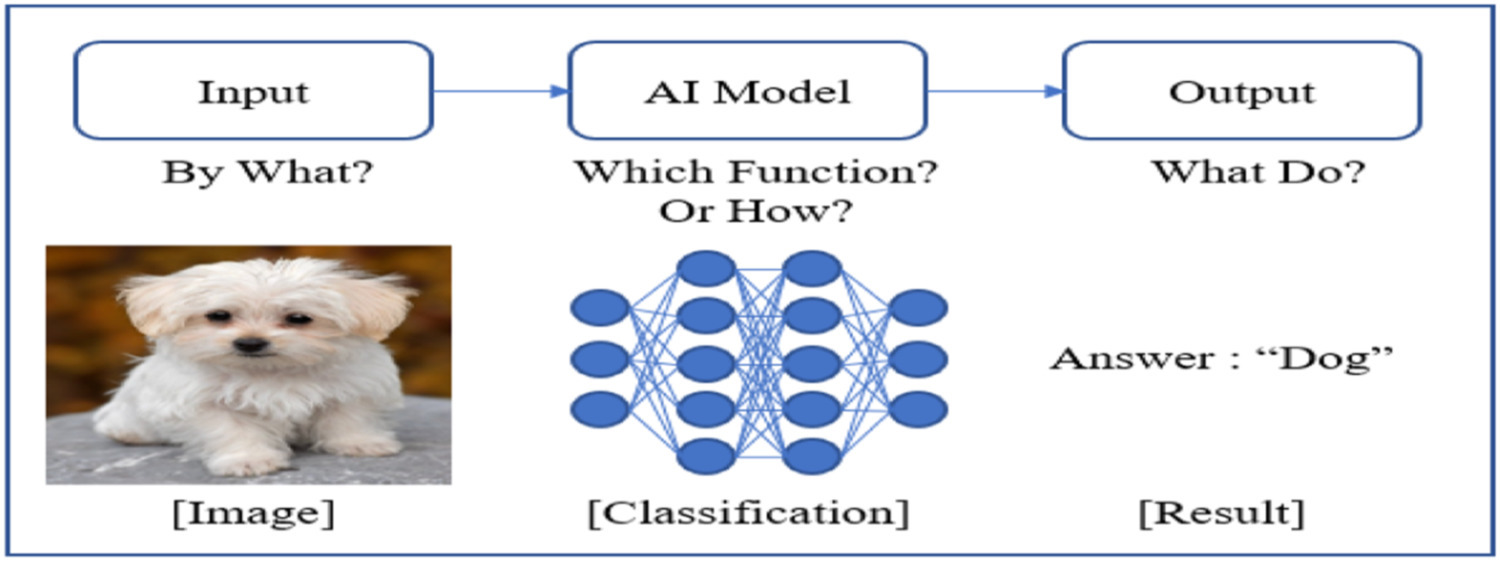
\includegraphics[width=0.5\textwidth]{image/fig 1.png}
                    \caption{مفهوم ساختار IMO}
                    \label{fig:fig_1}
            
                \end{figure}

            \subsubsection{چرا باید از ساختار IMO استفاده کرد؟}

                ساختار IMO یک ساختار منطقی است که ورودی و خروجی را به اطراف یک مدل هوش مصنوعی مرکز می‌کند. دلیل استفاده از ساختار IMO این است که یک مدل هوش مصنوعی نتیجه فناوری هوش مصنوعی است که از طریق داده و الگوریتم‌ها آموزش دیده شده است و موضوع عملکرد هوش مصنوعی است. حتی اگر چندین مدل هوش مصنوعی در سیستم راه‌اندازی و عمل کنند، هر مدل هوش مصنوعی از طریق ساختار IMO خود عمل می‌کند. ورودی مورد نیاز برای عملکرد مدل هوش مصنوعی همان معنی داده‌های مورد نیاز برای یادگیری یا عملکرد مدل هوش مصنوعی را دارد. خروجی نتیجه فناوری هوش مصنوعی است که مدل هوش مصنوعی از طریق داده‌های ورودی خروجی می‌دهد. به طور کلی، تمام ملاحظات طراحی برای پیاده‌سازی عملکرد هوش مصنوعی می‌تواند از طریق ساختار IMO مشتق شود. بنابراین، از منظر فنی، می‌توان ساختار IMO را به عنوان آغاز و پایان تشکیل فناوری هوش مصنوعی در نظر گرفت، و شناسایی ملاحظات طراحی برای فناوری هوش مصنوعی از طریق ساختار IMO منطقی به نظر می‌رسد.
    
            \subsubsection{ملاحظات فنی برای طراحی معماری سیستم هوش مصنوعی با استفاده از ساختار IMO}

                در این بخش، ملاحظات فنی برای طراحی سیستم‌ها و فناوری هوش مصنوعی با استفاده از ساختار IMO را شرح می دهیم. فناوری هوش مصنوعی به طور کلی به دو مرحله تقسیم می شود: فرآیند دستیابی به مدل های هوش مصنوعی و فرآیند بهره برداری از آنها. ساختار IMO در هر دو این مراحل گنجانده شده است، اما تفاوت در محیط است. محیطی که فرآیند دستیابی به مدل‌های هوش مصنوعی در آن انجام می‌شود، عمدتاً یک محیط آزمایشگاهی یا تحقیقاتی است، در حالی که محیطی که مدل هوش مصنوعی در آن اجرا می‌شود، سیستم واقعی است که مدل هوش مصنوعی در آن مستقر شده است. این تفاوت های محیطی در نهایت بر داده های مورد استفاده برای به دست آوردن مدل هوش مصنوعی و عملکرد مدل هوش مصنوعی به دست آمده تأثیر می گذارد. اگر این تفاوت‌ها در طول طراحی معماری نادیده گرفته شوند، مدل هوش مصنوعی ممکن است الزامات عملکرد را در مرحله اکتساب برآورده کند اما در مرحله عملیات واقعی سیستم نتواند آنها را برآورده کند. برای جلوگیری از این امر، در این مطالعه، ساختار IMO را از محیطی که سیستم هوش مصنوعی توسعه‌یافته در آن کار خواهد کرد، شناسایی کرده و از آن برای مشخص کردن الزامات فنی مرتبط با ساختار IMO در فرآیند دستیابی به مدل هوش مصنوعی استفاده می‌کنیم. برای نشان دادن اعتبار رویکردمان، توضیح می‌دهیم که چگونه ساختار IMO از نظر تئوری در هر دو فناوری هوش مصنوعی و دیدگاه‌های سیستم وجود دارد و آنچه باید بر اساس آن طراحی شود.

                \paragraph*{3.1.3.1}{دیدگاه فناوری هوش مصنوعی}
                
                    به دست آوردن فناوری هوش مصنوعی در نهایت به معنای به دست آوردن یک مدل هوش مصنوعی با عملکردهای مورد نظر است. فناوری‌های هوش مصنوعی به طور معمول به یادگیری نظارت شده، یادگیری بدون نظارت و یادگیری تقویتی تقسیم می‌شوند. فرآیند به دست آوردن این فناوری‌های هوش مصنوعی شامل به دست آوردن و عملکرد مدل‌های هوش مصنوعی است. شکل 2 هر فرآیند، روابط آن‌ها و مکان ساختار IMO را نشان می‌دهد. از آنجایی که فناوری هوش مصنوعی اساساً فناوری نرم‌افزاری است، زبان پایتون و دستورات کراس [20] برای توصیف آن استفاده شده است.

                    اولاً، همانطور که در سمت چپ شکل 2 نشان داده شده است، فرآیند به دست آوردن یک مدل هوش مصنوعی به طور کلی شامل سه مرحله است: آماده‌سازی آزمایش، طراحی الگوریتم هوش مصنوعی، آموزش و اعتبارسنجی، که معمولاً در یک محیط آزمایشگاهی انجام می‌شود. در مرحله آماده‌سازی آزمایش، داده‌های مورد نیاز برای یادگیری نظارت شده/بدون نظارت یا محیطی برای یادگیری تقویتی آماده می‌شود. سپس، در مرحله طراحی الگوریتم هوش مصنوعی، ساختار دقیق معماری IMO برای به دست آوردن مدل هوش مصنوعی طراحی می‌شود. ورودی‌ها به شکل شکل یا ابعادی که در الگوریتم هوش مصنوعی استفاده خواهد شد، طراحی می‌شوند. به عنوان مثال، در یادگیری نظارت شده/بدون نظارت، داده‌های پیش‌پردازش شده با اشکال یا ابعاد مشخص از تصاویر، صدا، یا متن به طور معمول استفاده می‌شود. این همچنین در مورد یادگیری تقویتی صادق است. با این حال، در یادگیری تقویتی، داده‌های به دست آمده از طریق وسایل مشاهده موجود در محیط طراحی شده برای عامل مانند دوربین‌ها یا رادارها استفاده می‌شود. الگوریتم‌های هوش مصنوعی از ترکیب لایه‌های شبکه عصبی مصنوعی مانند CNN، LSTM و Batchnormalization برای انجام عملکردهای مورد نظر تشکیل شده‌اند. سمت چپ شکل 2 مثالی از کد منبع کلی را نشان می‌دهد که الگوریتم یادگیری نظارت شده را به آن کمک می‌کند تا درک شود. خروجی عملکرد مورد نیاز توسط مدل هوش مصنوعی را نشان می‌دهد. به عنوان مثال، در یادگیری نظارت شده، این ممکن است یک برچسب مانند "سگ" باشد، و در یادگیری تقویتی، این ممکن است یک عمل مانند "حرکت به بالا" یا "حرکت به پایین" باشد. در نهایت، در مرحله آموزش و اعتبارسنجی، وظایف آموزش و اعتبارسنجی تکراری با استفاده از داده‌های (یا محیط) آماده‌شده و الگوریتم هوش مصنوعی انجام می‌شود. در یادگیری نظارت شده، یادگیری هوش مصنوعی عمدتاً با کاهش تفاوت بین خروجی الگوریتم هوش مصنوعی و حقیقت انجام می‌شود. در یادگیری بدون نظارت، یادگیری هوش مصنوعی بدون برچسب انجام می‌شود، اما هوش مصنوعی توزیع یا ویژگی‌های داده‌ها را به درستی یاد می‌گیرد تا به عنوان هدف توسط معمار هوش مصنوعی مورد نظر دسته‌بندی شود. در یادگیری تقویتی، یادگیری هوش مصنوعی با بیشینه کردن پاداش تجمعی حاصل از خروجی الگوریتم هوش مصنوعی در محیط انجام می‌شود. این مرحله تا زمانی که مدل هوش مصنوعی به معیارهای عملکرد کافی مانند دقت برسد، تکرار می‌شود. در نهایت، محصول نهایی کلیه فرآیند به دست آوردن یک مدل هوش مصنوعی، یک مدل هوش مصنوعی آموزش‌دیده به خوبی است.

                    دوماً، همانطور که در سمت راست شکل 2 نشان داده شده است، فرآیند عملکرد مدل هوش مصنوعی شامل دو مرحله است: بارگذاری مدل هوش مصنوعی و عملکرد مدل هوش مصنوعی. این فرآیند در یک سیستم در یک محیط عملیاتی واقعی انجام می‌شود. در مرحله بارگذاری مدل هوش مصنوعی، وظیفه بارگذاری مدل هوش مصنوعی آموزش‌دیده و الگوریتم‌های آن به حافظه سیستم است. سپس، در مرحله عملکرد مدل هوش مصنوعی، سیستم با استفاده از مقادیر ورودی از سیستم و مدل هوش مصنوعی بارگذاری شده، مقادیر خروجی را پیش‌بینی می‌کند. بزرگترین تفاوت بین این مرحله و مرحله به دست آوردن مدل هوش مصنوعی، داده است. در حالی که در فرآیند به دست آوردن مدل هوش مصنوعی از داده‌های آماده استفاده می‌شود، فرآیند عملکرد مدل هوش مصنوعی داده‌های ورودی را از سیستم واقعی دریافت می‌کند.

                    \begin{figure}[htbp]

                        \centering
                        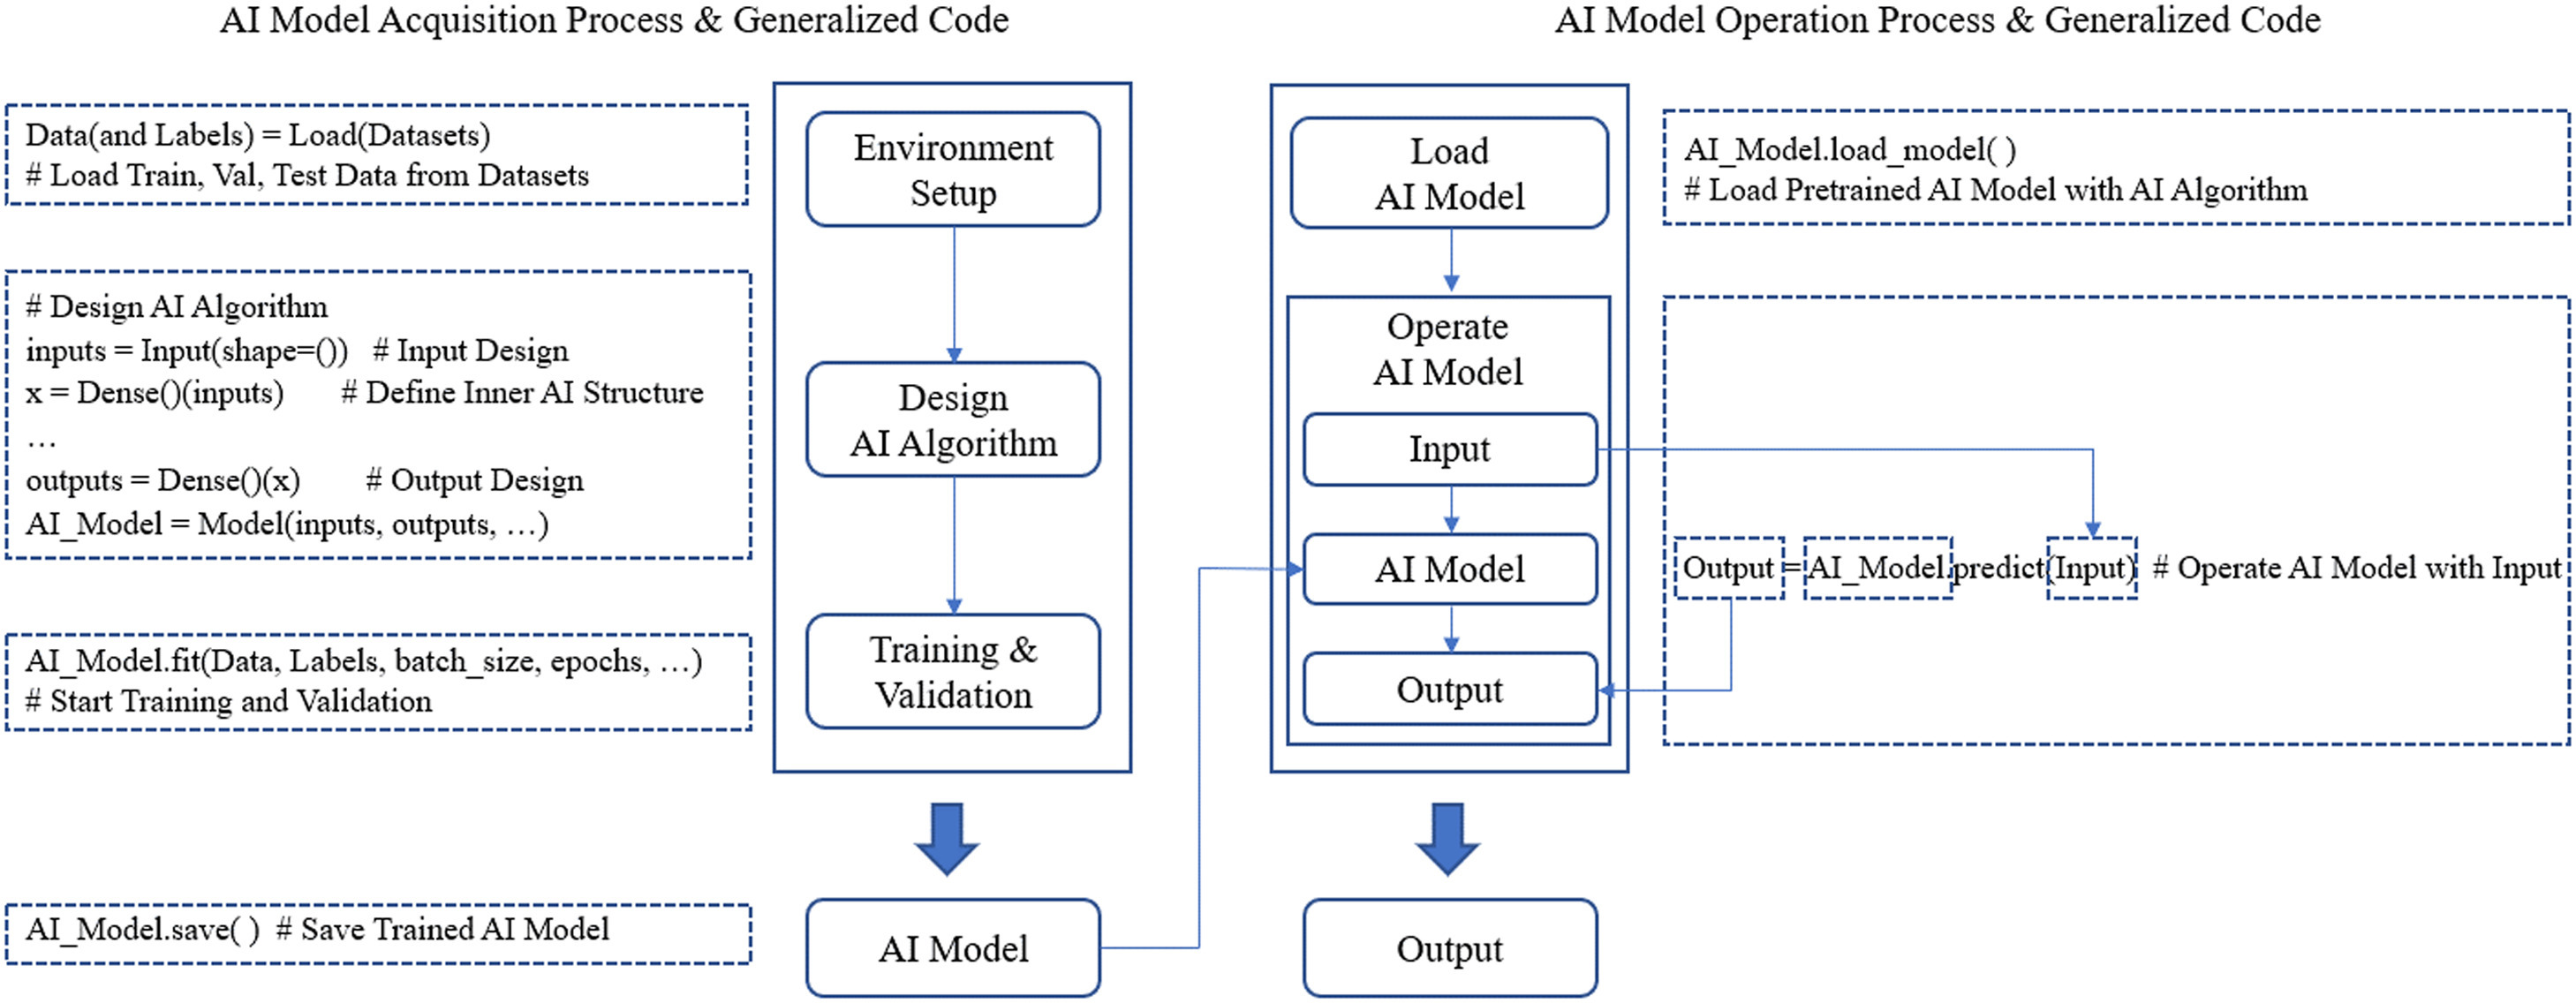
\includegraphics[width=0.8\textwidth]{image/fig 2.png}
                        \caption{فرآیند کسب و عملیات یک مدل هوش مصنوعی و موقعیت ساختار IMO}
                        \label{fig:fig_2}
                    
                    \end{figure}

                \paragraph*{3.1.3.2}{دیدگاه سیستمی}

                    سیستم دارای یک معنای گسترده است [[5], [6], [7],21,22]، اما به طور کلی می‌توان آن را به عنوان یک مجموعه متنوع از عناصر مرتبط که با همکاری با یکدیگر برای دستیابی به یک هدف مشترک کار می‌کنند، تعریف کرد. بسته به قصد طراح، سیستم از ترکیبی از عناصری که در سطوح مختلف موجود هستند، مانند زیرسیستم‌ها، اجزا و بخش‌ها، از طریق فرآیند تجزیه و تحلیل سیستم تشکیل شده است. در این زمینه، ممکن است اجزا به اشکال مختلفی مانند برقی، کنترل‌کننده‌ها، نرم‌افزار (SW) یا اشکال دیگر تعریف شوند، بسته به نقش اختصاص یافته در طراحی سیستم به عنوان یک زیرسیستم یا عنصر سطح پایین‌تر سیستم. برای کاهش پیچیدگی، توصیف زیرعناصر زیر سطح قسمت‌ها در این مطالعه حذف شده است. همانطور که قبلاً گفته شد، فناوری هوش مصنوعی یک فناوری نرم‌افزاری است که برای انجام عملکردهای خاصی مانند شناخت، تولید و رفتار طراحی شده است، و خروجی آن یک مدل هوش مصنوعی است. بنابراین، فناوری هوش مصنوعی در ماژول SW که مدل هوش مصنوعی استفاده می‌شود و در سطح اجزا SW نماینده می‌شود، وجود دارد. در این مقاله، آن را به عنوان یک مؤلفه هوش مصنوعی نام می‌دهیم. به طور خلاصه، از دیدگاه سیستم، یک سیستم هوش مصنوعی می‌تواند به عنوان یک سیستم با یک یا چند مؤلفه هوش مصنوعی تعریف شود، و یک مؤلفه هوش مصنوعی یک مؤلفه سیستم با یک یا چند ساختار IMO است. شکل 3 سلسله مراتب کلی سیستم هوش مصنوعی و چگونگی وجود ساختار IMO را نشان می‌دهد. ساختار SW شامل مدل هوش مصنوعی در شکل 3 یک مؤلفه هوش مصنوعی است، و سیستم و زیرسیستم حاوی مؤلفه هوش مصنوعی به ترتیب به عنوان سیستم‌های هوش مصنوعی و زیرسیستم‌های هوش مصنوعی نمایش داده می‌شوند.

                    \begin{figure}[htbp]

                        \centering
                        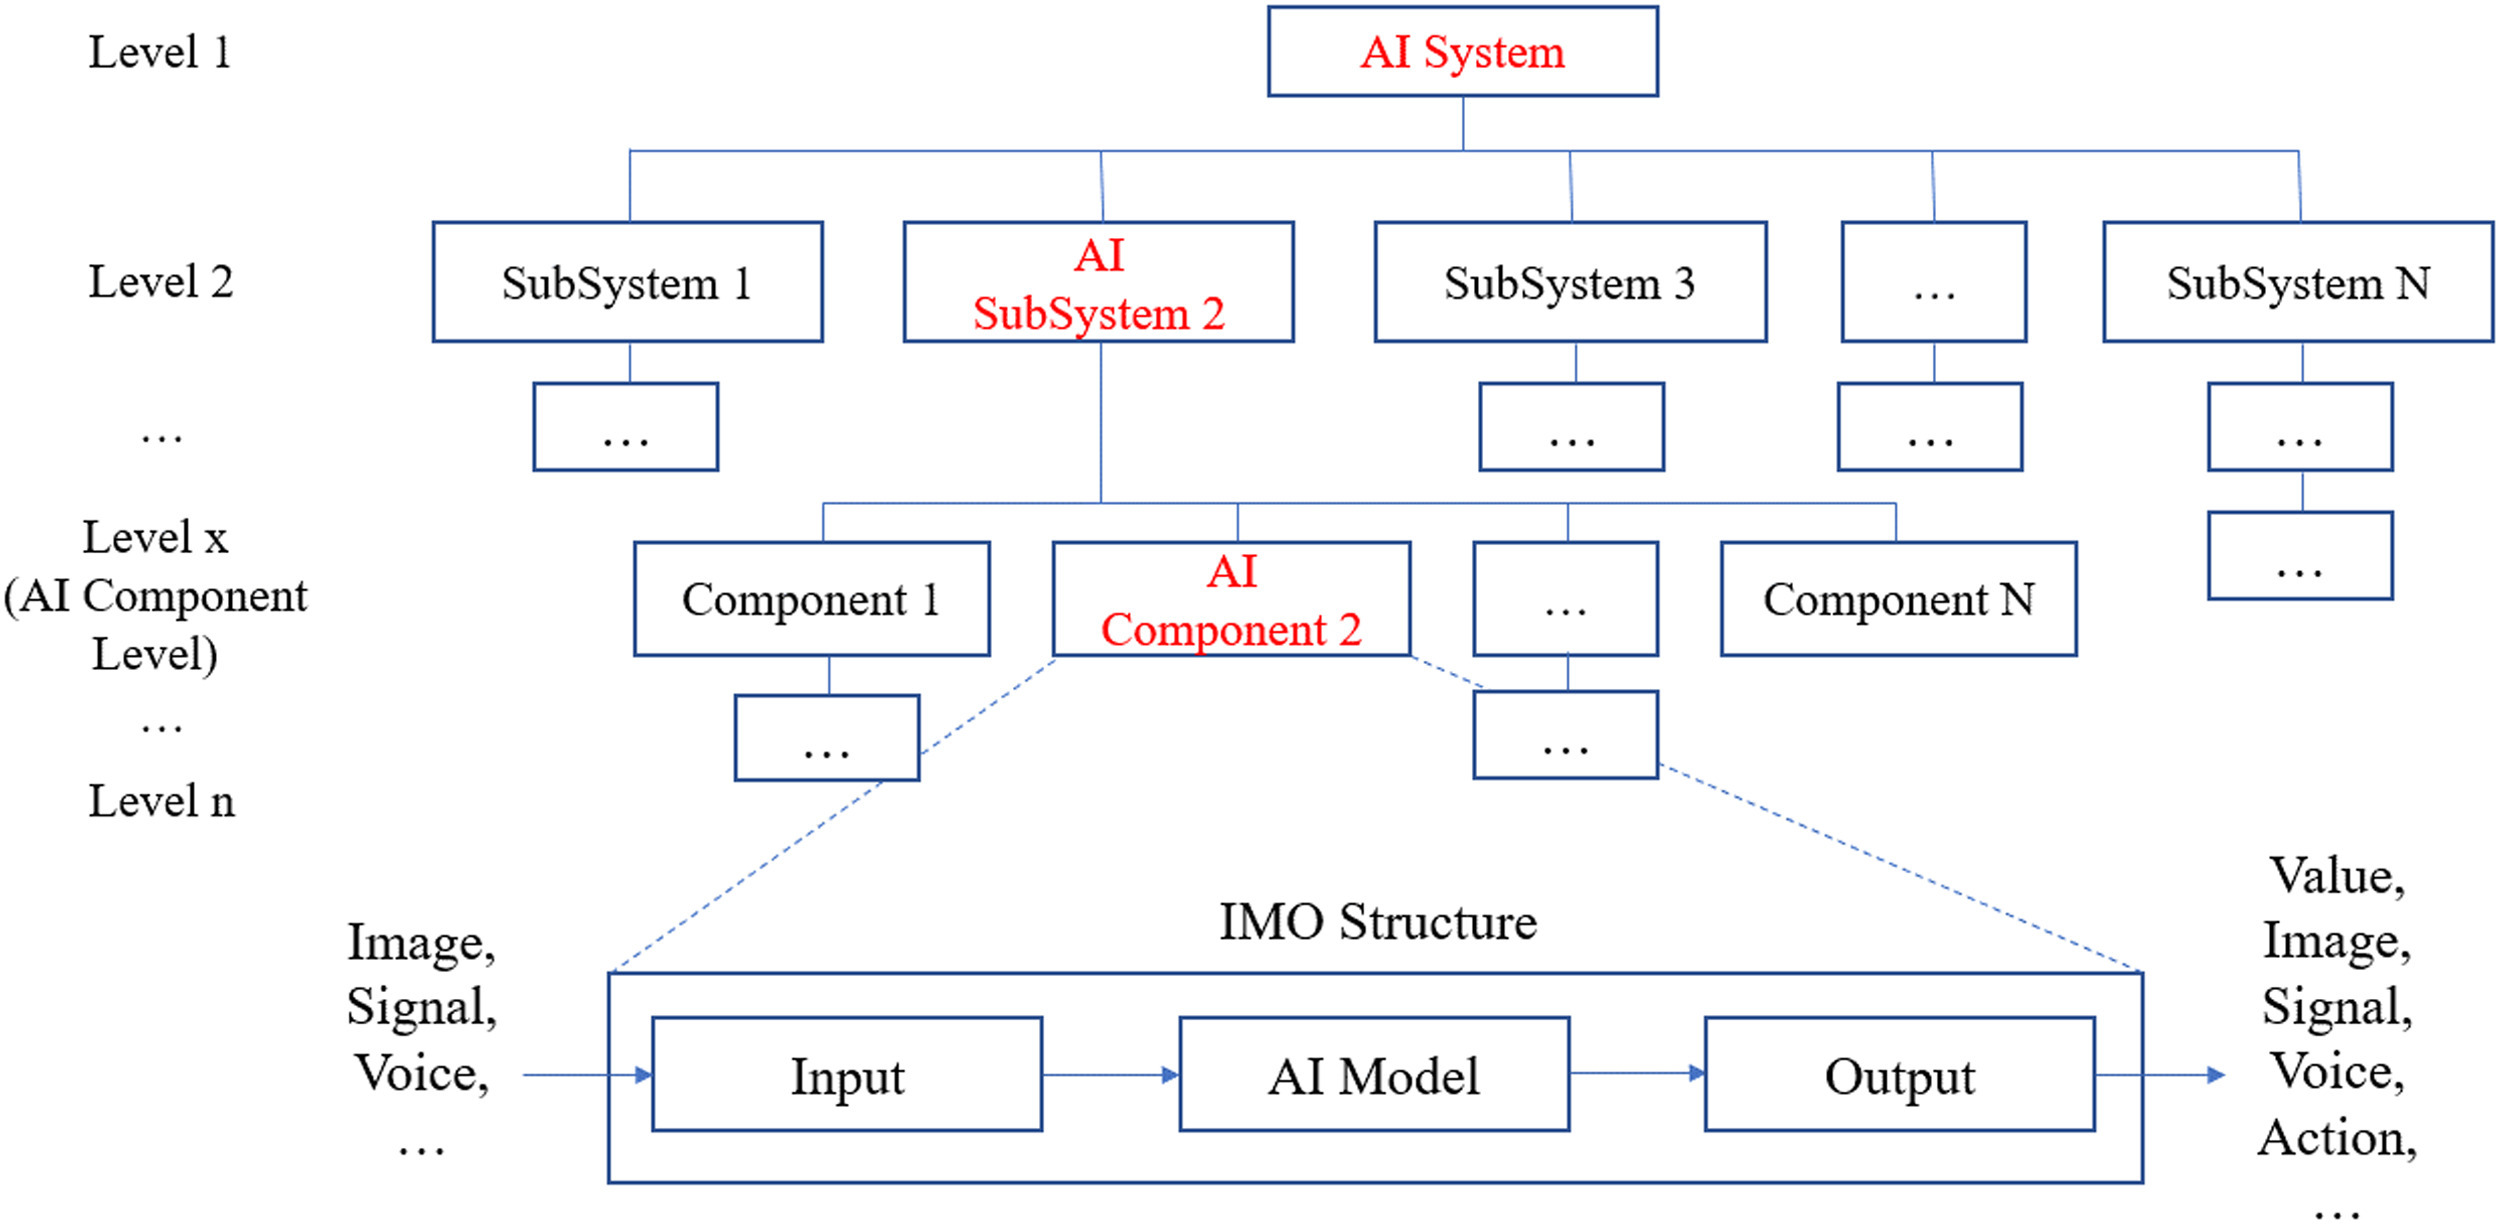
\includegraphics[width=0.6\textwidth]{image/fig 3.png}
                        \caption{سلسله مراتب یک سیستم هوش مصنوعی تعمیم یافته و مکان ساختار IMO}
                        \label{fig:fig_3}
                    
                    \end{figure}

                \paragraph*{3.1.3.3}{ملاحظات فنی برای طراحی معماری سیستم هوش مصنوعی}

                    در این بخش، ما در مورد ملاحظات فنی که باید هنگام ساختاردهی یک معماری سیستم هوش مصنوعی از طریق ساختار IMO شناسایی یا طراحی شوند توضیح می‌دهیم. ملاحظات فنی پیشنهاد شده در این مطالعه شامل چهار مورد می‌شود: داده یا محیط، الگوریتم هوش مصنوعی و خروجی، عملکرد هوش مصنوعی و الزامات مؤلفه هوش مصنوعی.

                    \begin{itemize}
                        
                        \item داده یا محیط: داده و محیط پیش‌نیازهای ضروری برای یادگیری الگوریتم‌های هوش مصنوعی هستند و با قسمت I از ساختار IMO ارتباط دارند. به طور کلی، فناوری هوش مصنوعی برای یادگیری نیاز به حجم زیادی از داده دارد و آماده‌سازی داده بیشترین زمان را در توسعه مدل هوش مصنوعی به خود اختصاص می‌دهد. علاوه بر این، داده تأثیر مستقیمی بر عملکرد مدل‌های هوش مصنوعی دارد. بنابراین، طراحی الزامات روشن برای داده یا محیط هنگام طراحی عملکرد هوش مصنوعی سیستم بسیار حیاتی است. همانطور که در بخش 3.1.3.1 مشاهده می‌شود، تفاوت اصلی بین فرآیندهای به دست آوردن و عملیات مدل‌های هوش مصنوعی داده ورودی است. در فرآیند به دست آوردن یک مدل هوش مصنوعی، ورودی داده آماده یا اطلاعاتی است که در یک محیط آماده‌سازی شده به دست آمده و عملکرد مدل هوش مصنوعی آموزش دیده را تعیین می‌کند. با این حال، در زمان عملیات مدل هوش مصنوعی، ورودی داده یا اطلاعاتی است که در محیط عملیاتی واقعی سیستم به دست آمده و عملکرد واقعی سیستم هوش مصنوعی را تعیین می‌کند. اگر داده یا اطلاعاتی که از محیط عملیاتی واقعی به دست می‌آید با داده یا محیطی که برای به دست آوردن مدل هوش مصنوعی استفاده شده است متفاوت باشد، مدل هوش مصنوعی آموزش دیده شده ممکن است عملکرد ضعیف یا رفتارهای نامطلوبی داشته باشد. بنابراین، هنگام طراحی معماری سیستم هوش مصنوعی، داده یا محیط باید بر اساس تجزیه و تحلیل محیط عملیاتی سیستم واقعی مشتق و تأیید شود.

                        \item الگوریتم‌های هوش مصنوعی و خروجی: به عنوان مواردی که می‌توانند به طور مستقیم به الزامات ذینفعان برای عملکرد هوش مصنوعی نقش ببینند، با مؤلفه‌های M و O از ساختار IMO مرتبط هستند. الگوریتم‌های هوش مصنوعی به الزامات ذینفعان برای "کدام عملکرد" سیستم هوش مصنوعی باید انجام دهد نقش می‌بیند، که ممکن است شامل عملکردهایی مانند طبقه‌بندی، شناسایی و تولید باشد. خروجی به الزامات ذینفعان برای "چگونگی ارائه عملکرد" نقش می‌بیند. به عنوان مثال، اگر الزامات ذینفعان برای شناسایی آبجکت‌ها به صورت زمان واقعی از تصاویر باشد، عملکرد هوش مصنوعی "شناسایی" خواهد بود و خروجی "موقعیت آبجکت در تصویر" خواهد بود. این‌ها می‌توانند به صورت محکم به برخی الگوریتم‌های هوش مصنوعی خاص مانند YOLO یا Faster R-CNN، که می‌توانند عملکرد "شناسایی" را انجام دهند، از طریق فرآیند طراحی معماری دقیق مواد شوند. و خروجی می‌تواند به اشکال مختلفی مانند "برچسب" و "جعبه‌ی محدود" نمایش داده شود.

                        \item کارایی هوش مصنوعی: به عملکرد یک مدل آموزش دیده هوش مصنوعی اشاره دارد و با عناصر M و O از ساختار IMO ارتباط دارد. روش‌های مختلفی برای اندازه‌گیری عملکرد یک مدل هوش مصنوعی وجود دارد که به نوع و هدف الگوریتم هوش مصنوعی بستگی دارد. بنابراین، الزامات عملکرد هوش مصنوعی باید روش اندازه‌گیری عملکرد مناسبی را انتخاب کنند که در حد امکان نیازهای ذینفعان را برآورده کند. به عنوان مثال، mAP به طور اصلی برای شناسایی آبجکت [23] استفاده می‌شود و WER به طور اصلی برای تشخیص گفتار استفاده می‌شود. با این حال، در یادگیری تقویتی، عملکرد یک عامل می‌تواند بسته به محیط پویایی تغییر کند، و در حال حاضر هیچ راه روشنی برای مقایسه عملکرد عوامل آموزش دیده وجود ندارد. تلاش‌های مختلفی برای حل این مسئله وجود دارد. اولین راه حل ایجاد بسیاری از محیط‌های استاندارد است که مشکلات هر دامنه را به وضوح نشان دهند. دومین راه حل توسعه انواع مختلفی از سناریوهای آزمایش استاندارد برای عوامل یادگیری تقویتی در هر محیط استاندارد است. در نهایت، نمودار پاداش تجمعی یک مدل هوش مصنوعی که در محیط‌ها و سناریوهای آزمایش استاندارد اندازه‌گیری شده‌است، می‌تواند به عنوان یک شاخص عملکرد پایداری مورد استفاده قرار گیرد. این نمودار پاداش هر مقدار پاداشی را که عامل در طول فرآیند یادگیری به دست آورده است نمایش می‌دهد. اگر این نمودار ارزش‌های پاداش بالایی را در محیط‌ها و سناریوهای آزمایش استاندارد مختلف به طور پایدار حفظ کند، مدل هوش مصنوعی آموزش دیده شده را پایدار می‌توان در نظر گرفت.

                        \item الزامات مؤلفه‌های هوش مصنوعی: به الزامات سطح سیستم برای عملکرد مدل‌های هوش مصنوعی تهیه شده می‌پردازد، که شامل مؤلفه‌های نرم‌افزاری (SW) مانند سیستم عامل (OS) و مؤلفه‌های سخت‌افزاری (HW) مانند واحد پردازش مرکزی (CPU) و حافظه دسترسی تصادفی (RAM) می‌شود. الزامات مؤلفه‌های هوش مصنوعی با طراحی منابع محاسباتی لازم مرتبط بوده و در نهایت بر روی هزینه تولید سیستم‌های هوش مصنوعی تأثیر می‌گذارد. به طور کلی، برای فرآیند تهیه مدل هوش مصنوعی، منابع محاسباتی با عملکرد بالا لازم است. با این حال، برای فرآیند عملکرد مدل هوش مصنوعی، منابع محاسباتی با عملکرد نسبتاً پایین لازم است. در فرآیند تهیه مدل هوش مصنوعی، داده‌ها یا محیطی که برای آموزش آماده شده‌اند، به حافظه سیستم بارگذاری شده و وزن‌های مدل هوش مصنوعی به‌طور مکرر محاسبه و به‌روزرسانی می‌شود. در حالی که فرآیند عملکرد مدل هوش مصنوعی تنها نیاز به استنتاج با استفاده از مدل هوش مصنوعی آموزش دیده دارد. بسیاری از مطالعات در حال انجام است برای پوشش دادن نقص منابع محاسباتی با عملکرد بالا برای عملکرد مدل‌های هوش مصنوعی. به عنوان مثال، مطالعات مختلفی عملکرد استنتاج به‌روز مدل هوش مصنوعی حتی در محیط‌های با عملکرد پایین مانند CPUs یا گوشی‌های همراه را نشان داده‌اند. بنابراین، هنگام طراحی معماری سیستم، مشخصات HW مناسب برای عملکرد مدل هوش مصنوعی آموزش دیده باید مدنظر قرار گیرد تا هزینه را در نظر بگیرد، یا تکنولوژی‌های هوش مصنوعی که حتی در محیط‌های با عملکرد پایین هم قابل عملیات هستند، باید مورد بررسی قرار گیرد.

                    \end{itemize}
        
        \subsection{فرآیند طراحی معماری سیستم هوش مصنوعی پیشنهادی}

            در این بخش، فرآیند طراحی معماری سیستم هوش مصنوعی را با تمرکز بر روی ساختار IMO شرح می‌دهیم. روش طراحی معماری پیشنهادی هدفش شناسایی و طراحی الزامات فنی برای سیستم‌ها و فناوری‌های هوش مصنوعی لازم از فعالیت‌های عملیاتی آینده است که می‌توانند به دستاوردهای سازمان برسند.

            \subsubsection{فرآیند اساسی}

                منهجی که ما ارائه داده‌ایم از سه فعالیت تشکیل شده است: تعریف مسئله، راه‌حل هوش مصنوعی سیستمی، و راه‌حل فنی هوش مصنوعی. شکل ۴ فرآیند پیشنهادی طراحی معماری سیستم هوش مصنوعی را نشان می‌دهد. فعالیت اول تعریف مسئله است. هدف این فعالیت مشخص کردن وضعیت مسئله و جایگزینی است که سازمان می‌خواهد از منظر عملیاتی به آن پرداخته شود. در این مرحله، مسائل سازمان و نقش‌های هوش مصنوعی برای حل مسائل شناسایی می‌شوند. فعالیت دوم، راه‌حل هوش مصنوعی سیستمی، هدف طرح‌های مشخص‌شده که می‌توانند الزامات سازمان را که از منظر عملیاتی شناسایی شده‌اند، از دیدگاه سیستمی به تجسم در آورد. در این مرحله، ساختار سیستم و الزامات عنصر هوش مصنوعی که می‌توانند نقش‌های هوش مصنوعی شناسایی شده را انجام دهند، مشخص می‌شود. فعالیت آخر، راه‌حل فنی هوش مصنوعی، هدف تشخیص الزامات فنی برای به دست آوردن فناوری هوش مصنوعی است که می‌تواند نقش‌های هوش مصنوعی شناسایی شده را انجام دهد. در این مرحله، داده‌ها و عملکردهای هوش مصنوعی مورد نیاز برای توسعه مدل‌های هوش مصنوعی که در سیستم واقعی منافع استفاده خواهند شد، مشخص می‌شود.

                \begin{figure}[htbp]

                    \centering
                    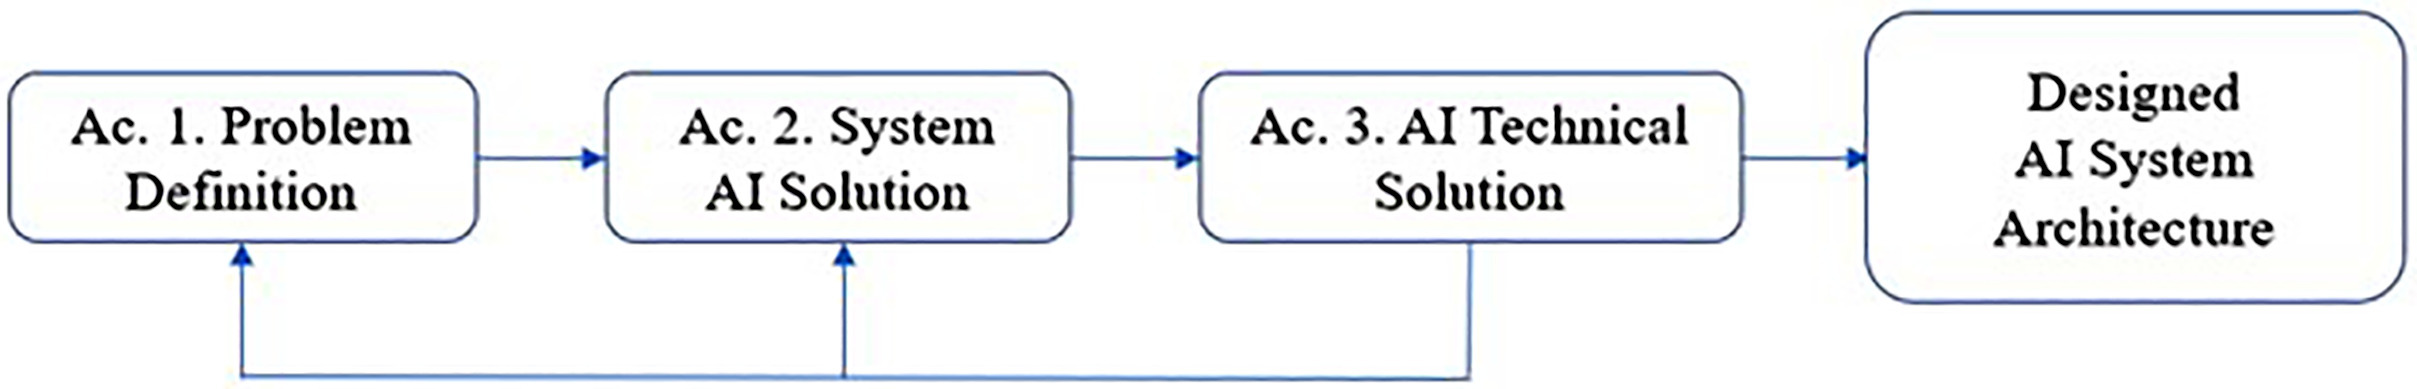
\includegraphics[width=0.6\textwidth]{image/fig 4.png}
                    \caption{فرآیند اساسی روش طراحی معماری سیستم هوش مصنوعی پیشنهادی}
                    \label{fig:fig_4}
                
                \end{figure}
            
                همانطور که در فصل 2 بررسی شد، طراحی معماری از طریق فعالیت‌های مهندسی سیستم معمولاً بر روی راه‌حل‌های سیستم تمرکز دارد. به عنوان مثال، چارچوب‌های موجود مانند DoDAF روش‌هایی برای تعریف دیدگاه‌های مختلف عملیاتی یا سیستمی ارائه می‌دهند، اما دیدگاه‌های برای بیان فناوری‌ها مانند StdV خاص نیستند و روش‌های شرح روشنی فراهم نمی‌کنند. به عنوان نتیجه، مطالعات موجود با استفاده از چارچوب‌های معمولی در شناسایی فناوری‌های هوش مصنوعی انتزاع بالایی را نشان می‌دهند. برای رفع این محدودیت‌ها، منهج ما با استفاده از درنظر گرفتن الزامات فنی مشتق شده از ساختار IMO، فناوری‌های هوش مصنوعی را مشخص می‌کند. سه فعالیت تا زمان کامل شدن طراحی معماری مکرر می‌شوند، که منجر به طراحی نهایی معماری سیستم هوش مصنوعی می‌شود.

            \subsubsection{فرآیند دقیق}

                در این بخش، جزئیات فرآیند پیشنهادی منهج را توضیح می‌دهیم. شکل 5 رابطه میان سه فعالیت طراحی پیشنهادی را نشان می‌دهد. هر فعالیت طراحی از خروجی اصلی خود استفاده می‌کند. فرآیند طراحی پیشنهادی به صورت مکرر از طریق همکاری کارشناسان حوزه، سیستم و هوش مصنوعی انجام می‌شود تا خروجی‌های اصلی هر مرحله به اندازه کافی بهبود یابند.

                \begin{figure}[htbp]

                    \centering
                    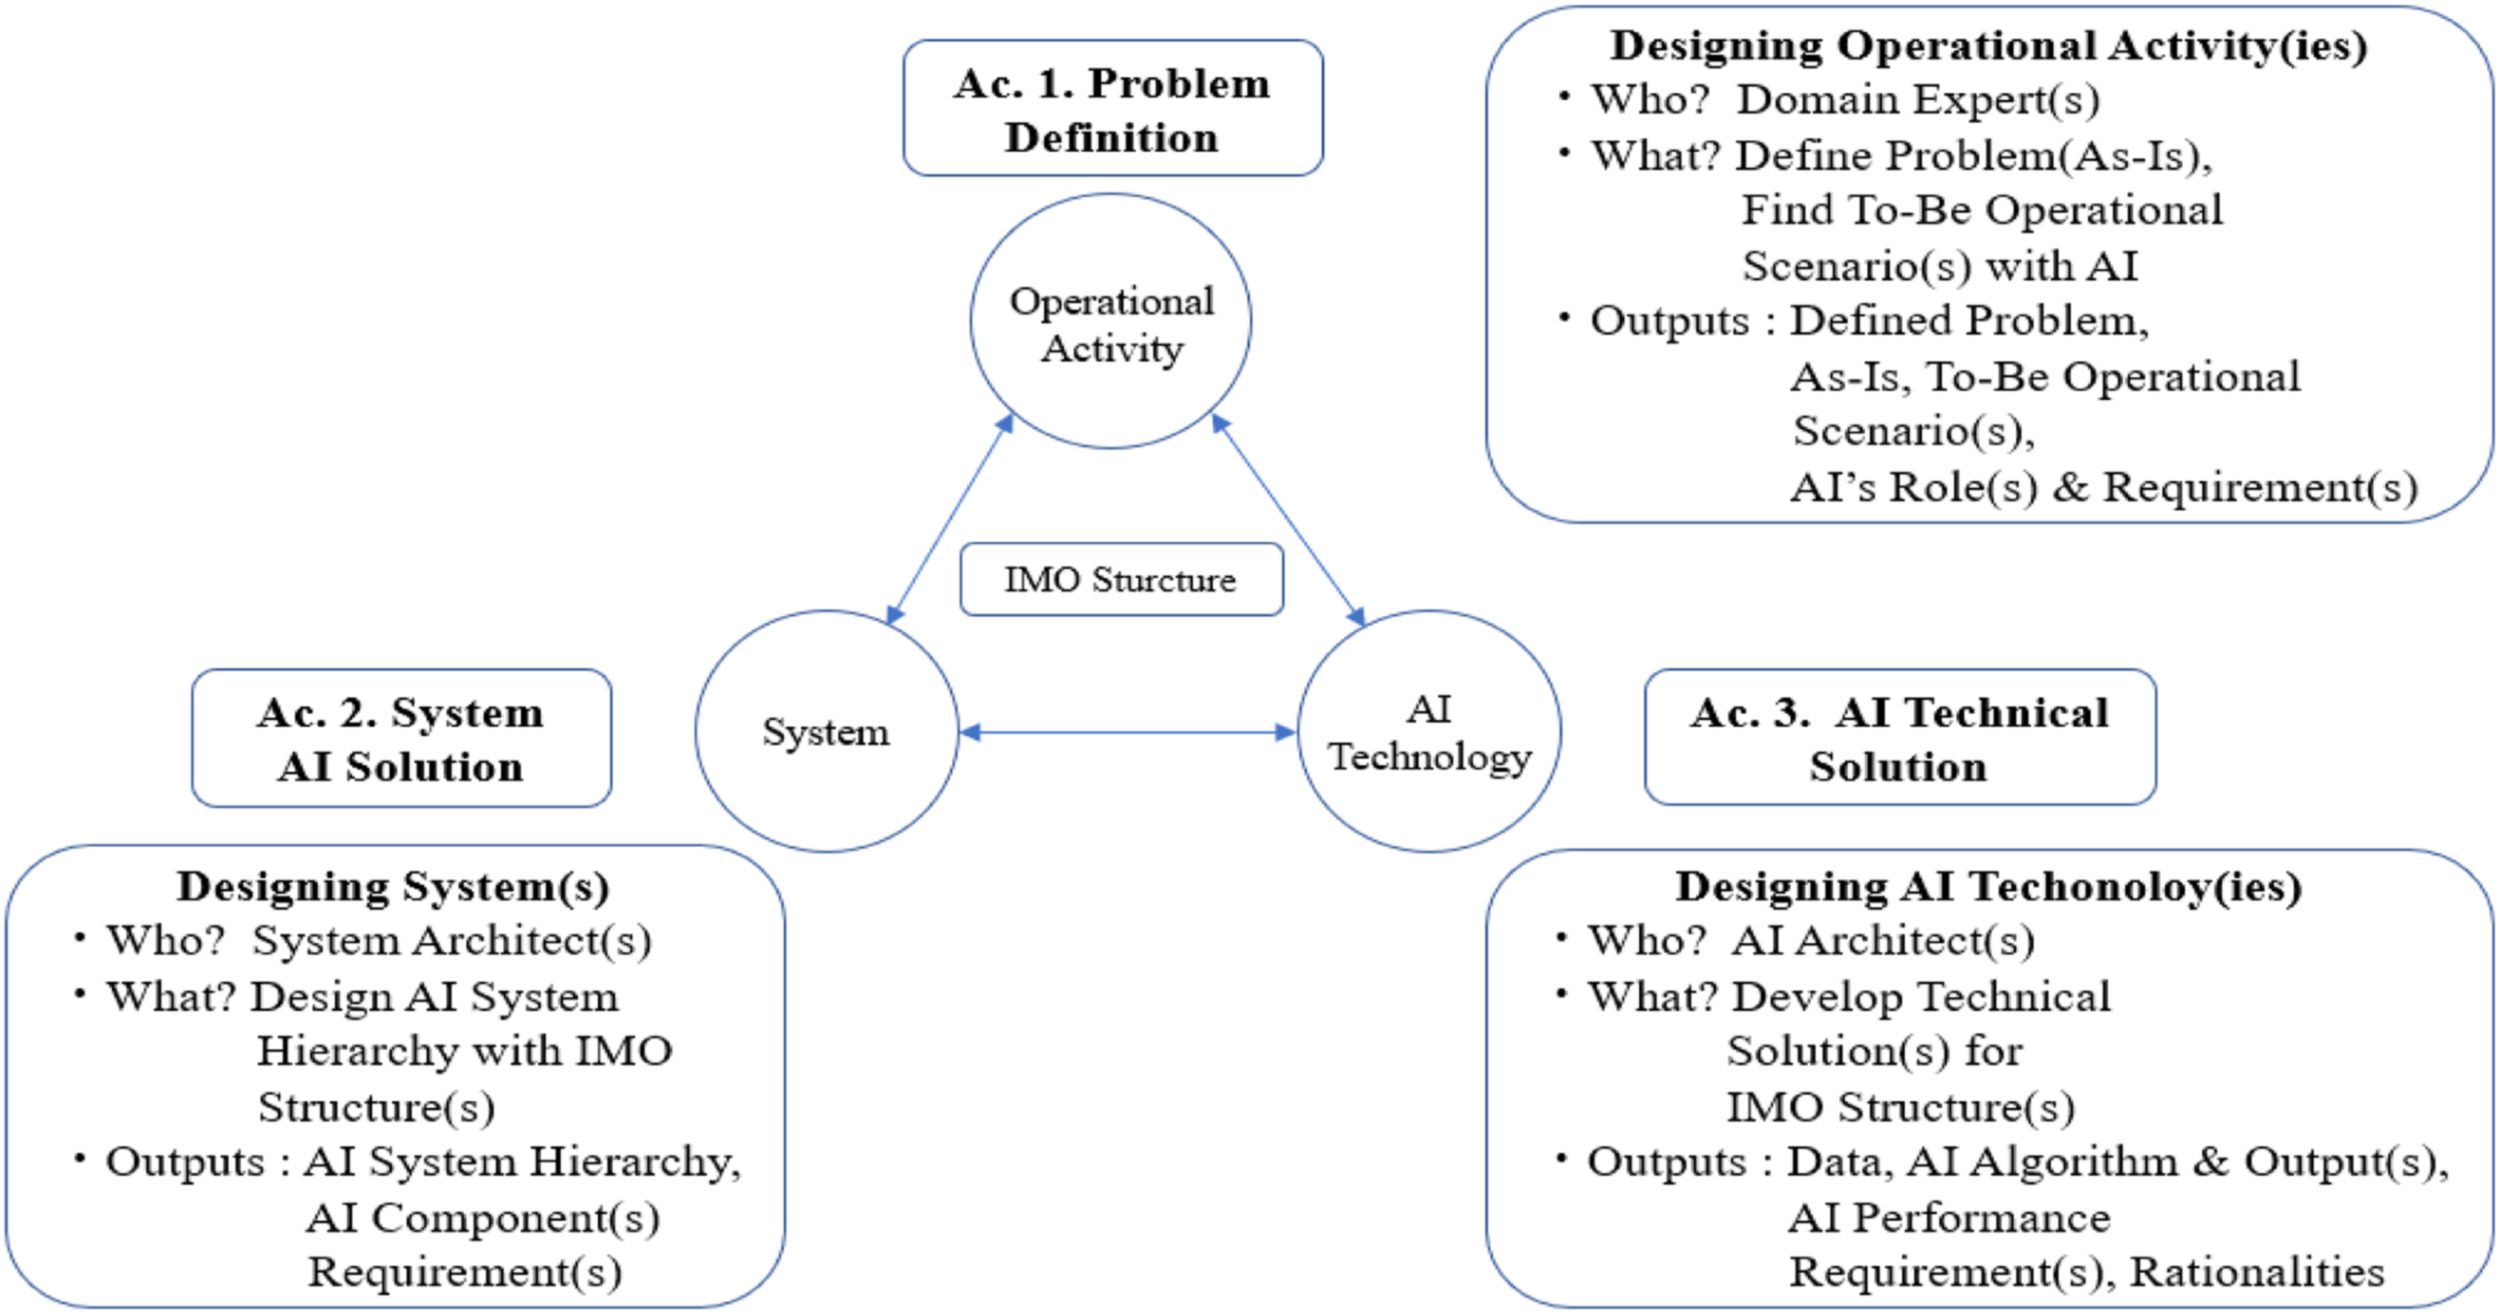
\includegraphics[width=0.8\textwidth]{image/fig 5.png}
                    \caption{رابطه متقابل بین سه فعالیت طراحی پیشنهادی}
                    \label{fig:fig_5}
                
                \end{figure}

                \paragraph{3.2.2.1}{مرحله تعریف مسئله Ac.1}

                    در مرحله تعریف مسئله، مسائلی که در حوزه تخصصی سازمان باید مورد توجه قرار گیرند، از طریق فعالیت‌های عملیاتی تعریف می‌شوند و نقش هوش مصنوعی بر اساس آن‌ها مشخص می‌شود. از آنجا که این مرحله به مسائل در حوزه تخصصی می‌پردازد، اصولاً توسط کارشناسان حوزه انجام می‌شود و از طریق چهار فعالیت جزئی انجام می‌شود که در شکل 6 زیر نشان داده شده است.

                    \begin{figure}[htbp]

                        \centering
                        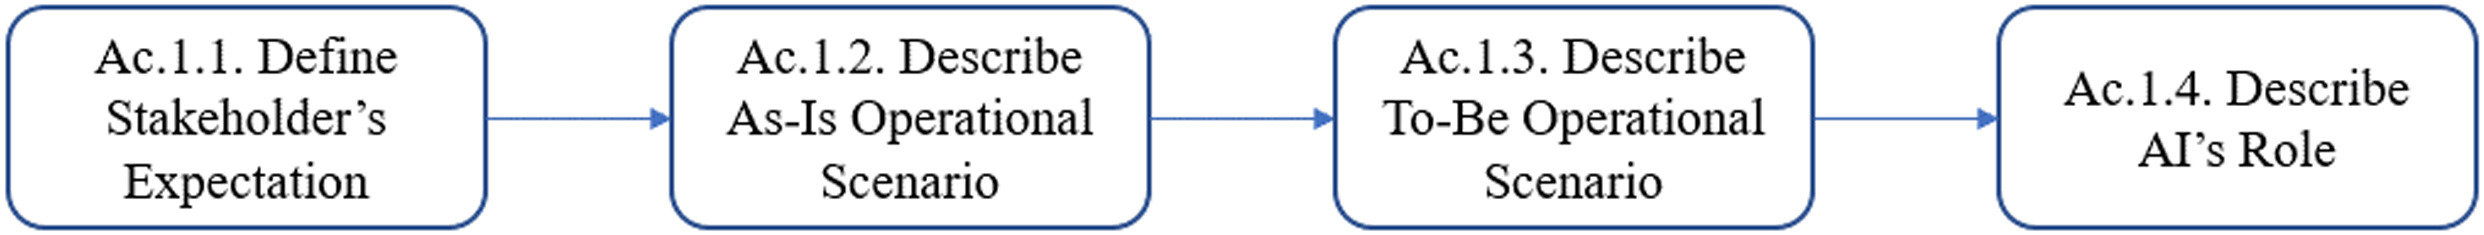
\includegraphics[width=0.8\textwidth]{image/fig 6.png}
                        \caption{رابطه متقابل بین سه فعالیت طراحی پیشنهادی}
                        \label{fig:fig_6}
                    
                    \end{figure}

                    جدول ۱ زیر نشان دهنده خروجی‌های اصلی است که باید در مرحله تعریف مسئله شناسایی شوند. شرح توضیحات جزئی هر فعالیت که خروجی‌های اصلی را مشخص می‌کند، به شرح زیر است.

                    \begin{table}[htbp]
                        
                        \centering
                        \caption{خروجی‌های اصلی مرحله تعریف مسئله}
                        \begin{tabularx}{\textwidth}{X}
                        
                            \specialrule{1pt}{1pt}{5pt}
                            \multicolumn{1}{c}{انتظارات ذینفعان [Ac.1.1.]} \\
                            \specialrule{0.5pt}{1pt}{1pt}
                            
                            شرح: مسئله‌هایی که باید با استفاده از هوش مصنوعی حل شوند را توصیف کنید یا تعریف کنید. \\
                            
                            \specialrule{0.5pt}{1pt}{5pt}
                            \multicolumn{1}{c}{سناریو(های) as-is [Ac.2.1.]} \\
                            \specialrule{0.5pt}{1pt}{1pt}
                            
                            شرح: مسائل فعلی که باید با استفاده از هوش مصنوعی حل شوند را به عنوان یک یا چند سناریو عملی از طریق روش‌های مناسب مانند EFFBD(s) و متن‌ها بیان کنید. \\
                            شرایط: عواملی که بر سناریو(های) عملی تأثیر می‌گذارند مانند زمان، فضا و سایر موارد را شرح دهید. \\
                            
                            \specialrule{0.5pt}{1pt}{5pt}
                            \multicolumn{1}{c}{سناریو(های) to-be [Ac.3.1.]} \\
                            \specialrule{0.5pt}{1pt}{1pt}
                            
                            شرح: بیان کنید سناریو(های) عملی آینده که مسئله(ها) با استفاده از هوش مصنوعی حل می‌شود(ند)، از طریق روش‌های مناسب مانند EFFBD(s) و متن. \\
                            شرایط: عواملی که بر سناریو(های) عملی تأثیر می‌گذارند، مانند زمان، فضا و سایر موارد را شرح دهید. \\
                            
                            \specialrule{0.5pt}{1pt}{5pt}
                            \multicolumn{1}{c}{نقش(های) هوش مصنوعی} \\
                            \specialrule{0.5pt}{1pt}{1pt}
                            
                            شرح: نقش(های) و اجرا کننده(ها) های هوش مصنوعی مورد نیاز برای سناریو(های) عملی آینده را (با در نظر گرفتن عنصر M و عنصر O از ساختار IMO) بیان کنید. \\
                            
                            \specialrule{1pt}{1pt}{1pt}
                            
                        \end{tabularx}
                    \end{table}

                    فعالیت اول، تعیین انتظارات سهام‌داران است (ارجاع داده شود به [Ac.1.1] در جدول ۱). سهام‌داران می‌توانند کاربران، توسعه‌دهندگان، یا افرادی باشند که نقش‌های مهمی در سیستم دارند یا مشکلاتی درباره آن دارند. برای اهداف این مطالعه، سهام‌داران کلیدی در این مرحله ممکن است کارشناسان حوزه باشند که عملیاتی یا رهبران در سازمان هستند. انتظارات سهام‌داران این است که با استفاده از هوش مصنوعی مشکلات فعلی را حل کنند. به عنوان مثال، در حال حاضر در حین ماموریت‌های مهار حریق، آتش‌نشانان، در آینده ممکن است از ربات‌های هوش مصنوعی برای ایمنی آتش‌نشانان استفاده کنند. در فعالیت‌های دوم و سوم، وضعیت "همانا" فعلی سازمان به عنوان مشکلاتی که باید حل شوند، بیان می‌شود و وضعیت "می‌خواهیم" به عنوان سناریوی عملیاتی آینده که در آن این مشکلات حل شده‌اند، بیان می‌شود (ارجاع داده شود به [Ac.2.1]، [Ac.3.1] در جدول ۱). سناریوهای عملیاتی ممکن است از روش‌های مختلفی مانند متن یا EFFBD [5] استفاده کنند تا بهترین نمایش مشکلات سازمان را داشته باشند. این فرآیند مشابه توسعه OV در DoDAF است. سناریوهای عملیاتی باید تجزیه و تحلیل دقیقی از اجراکنندگانی که فعالیت‌های عملیاتی را انجام می‌دهند و جریان منابع در یک مسئله داده شده را فراهم کنند تا مشکلات به طور کافی توضیح داده شوند. به علاوه، شرایطی که طرف‌های اجرایی می‌توانند فعالیت‌های خود را انجام دهند باید به طور همزمان تعریف شوند. به عنوان مثال، اگر طرف‌های اجرایی اتومبیل باشند، شرایط ممکن شامل زمانی است که اتومبیل می‌تواند فعالیت خود را انجام دهد (روز یا شب)، موقعیت (شهر یا کوهستان) و عوامل دیگر (شرایط جوی و غیره) باشد. این اطلاعات در نهایت با طراحی نیازمندی‌های داده برای ایمن کردن مدل‌های هوش مصنوعی از طریق تعریف محیط یا محدودیت‌هایی که زیر آن‌ها طرف‌های اجرایی می‌توانند فعالیت‌های خود را انجام دهند، مرتبط است. در فعالیت نهایی، نقش هوش مصنوعی و اجراکننده آن در سناریوی عملیاتی "می‌خواهیم" تعریف می‌شود (ارجاع داده شود به [Ac.4.1] در جدول ۱). نقش هوش مصنوعی با عناصر M و O از ساختار IMO تطابق داده می‌شود، بنابراین نقش هوش مصنوعی باید به اندازه‌ی ممکن به طور خاص مشخص یا تعریف شود تا عناصر M و O شناسایی شوند. به عنوان مثال، عنصر M می‌تواند از طریق فعل‌هایی مانند 'تشخیص \textasciitilde' یا 'پیشنهاد \textasciitilde' بیان شود و عنصر O می‌تواند از طریق اشیای مانند 'هدف‌ها' یا 'فیلم‌ها' بیان شود.

                \paragraph{3.2.2.2}{مرحله حل AI سیستم Ac.2}

                    مرحله راه‌حل هوش مصنوعی سیستم، سناریوی عملیاتی "می‌خواهیم" طراحی شده از منظر اجراکنندگان در مرحله تعریف مسئله را به یک منظر سیستم تبدیل می‌کند. به عنوان مثال، اگر یک سیستم رباتیک برای تعیین حضور بازماندگان در یک ساختمان که در آن حریق اتفاق افتاده است نیاز باشد، ربات منابع محاسباتی برای اجرای حسگرهایی مانند دید در شب یا رادار که قابلیت تشخیص انسان را دارند و یک مدل هوش مصنوعی را نیاز دارد. در این فرآیند، ساختار و طراحی عملکردی یک سیستم که می‌تواند انتظارات سهام‌داران را برآورده کند، انجام می‌شود و اجزای سیستم برای استقرار مدل هوش مصنوعی شناسایی می‌شوند. این مرحله اصولاً توسط کارشناسان سیستم انجام می‌شود و از طریق چهار فعالیت دقیق که در شکل 7 زیر نشان داده شده، انجام می‌شود.

                    \begin{figure}[htbp]

                        \centering
                        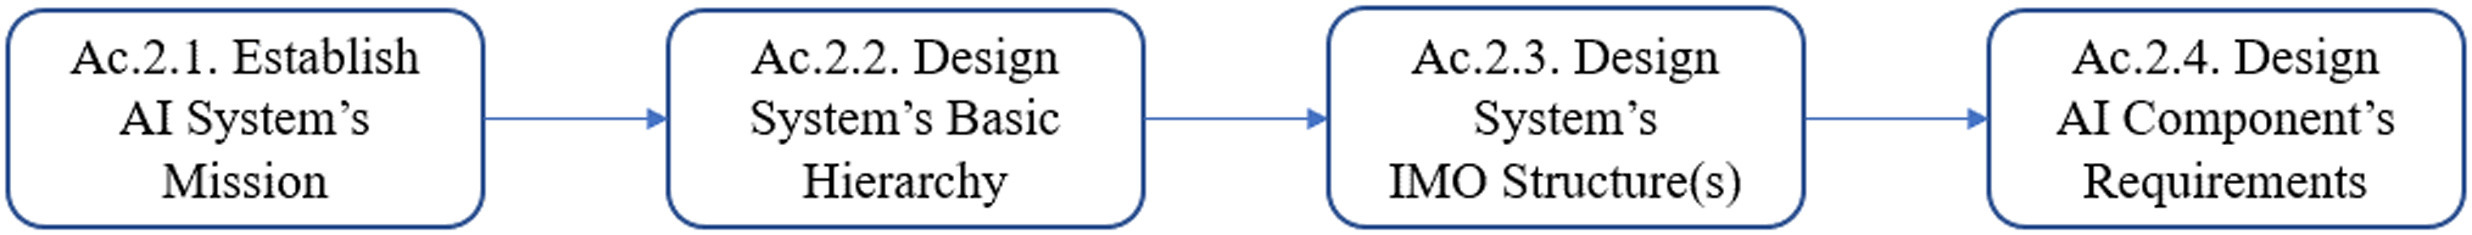
\includegraphics[width=0.8\textwidth]{image/fig 7.png}
                        \caption{چهار فعالیت در مرحله راه حل هوش مصنوعی سیستم}
                        \label{fig:fig_7}
                    
                    \end{figure}

                    جدول 3، خروجی‌های اصلی مرحله راه‌حل هوش مصنوعی سیستم را نشان می‌دهد. توضیحات دقیق هر فعالیت که خروجی‌های اصلی را واقعیت‌پذیر می‌کنند، به شرح زیر است.

                    در فعالیت اول، مأموریت سیستم مورد نیاز با ویژگی‌های هوش مصنوعی بر اساس سناریوی "می‌خواهیم" تعریف می‌شود. سیستم مورد نیاز با اجراکننده سناریوی عملیاتی آینده تطابق داده می‌شود (ارجاع داده شود به [Ac.1.2] در جدول ۲). به عنوان مثال، در مورد یک سیستم پهپاد برای نظارت بر حریق‌ها با استفاده از هوش مصنوعی، پهپاد سیستم مورد نظر است و مأموریت سیستم مورد نظر کشف حریق است. در فعالیت دوم، طراحی اولیه سیستم مورد نظر انجام می‌شود (ارجاع داده شود به [Ac.2.2] در جدول ۲). تجزیه و تحلیل سیستم [5] با توجه به جنبه‌های ساختاری، عملکردی و منطقی که برای طراحی ویژگی‌های هوش مصنوعی در سیستم مورد نظر لازم است، انجام می‌شود. تجزیه و تحلیل سیستم می‌تواند بسته به پیچیدگی سیستم مورد نظر به صورت عمیق‌تر انجام شود. با این حال، از آنجا که فرآیند طراحی معماری پیشنهادی با دامنه طراحی ویژگی‌های هوش مصنوعی سروکار دارد، تجزیه و تحلیل سیستم تنها تا سطح لازم برای طراحی ویژگی‌های هوش مصنوعی و نه کلیت ساختار سیستم انجام می‌شود. در فعالیت سوم، ساختار IMO از طریق سلسله مراتب سیستم مورد نظر طراحی می‌شود (ارجاع داده شود به [Ac.3.2] در جدول 2). این فعالیت اجزایی را که قادر به اجرای ویژگی‌های هوش مصنوعی مورد نیاز در سیستم هستند، شناسایی می‌کند و جریان اطلاعات را تعریف می‌کند. در این فرآیند، جریان اطلاعات داخل سیستم با پیکان‌ها ($\rightarrow$) نشان داده می‌شود. عنصر I از اجزای سیستم که اطلاعات داده را برای انجام ویژگی‌های هوش مصنوعی فراهم می‌کند، مشخص می‌شود. عنصر M از نقش هوش مصنوعی که در مرحله تعریف مسئله شناسایی شده است، مشخص می‌شود. عنصر O خروجی‌های مورد نیاز مدل هوش مصنوعی برای انجام ویژگی‌های هوش مصنوعی را مشخص می‌کند و از طریق یک فرآیند که اجزای سیستم را که تحت تأثیر خروجی‌های مدل هوش مصنوعی قرار می‌گیرند شناسایی و متصل می‌کند، واقعیت‌پذیر می‌شود. می‌توان برای اجرای ویژگی‌های هوش مصنوعی از اجزای مختلفی استفاده کرد. به عنوان مثال، در مورد خودروهای خودران، حسگرهایی مانند رادار، لیدار و دوربین‌ها اصلی استفاده می‌شوند. طراحی اجزای سیستم در نهایت با هزینه تولید سیستم مرتبط است، بنابراین این فعالیت همزمان با مرحله بعدی مرحله راه‌حل فناوری هوش مصنوعی انجام می‌شود تا راه‌حل بهینه را پیدا کند. در فعالیت نهایی، نیازمندی‌های سطح سیستم برای اجزای هوش مصنوعی که مدل هوش مصنوعی تعریف شده در آن‌ها استقرار و عملیاتی خواهد شد طراحی می‌شوند (ارجاع داده شود به [Ac.4.2] در جدول 2). این شامل مواردی مانند نیازمندی‌های نرم‌افزار (نرم‌افزار) و سخت‌افزار (سخت‌افزار) است.

                    \begin{table}[htbp]
                        
                        \centering
                        \caption{خروجی‌های اصلی مرحله راه حل هوش مصنوعی سیستم}
                        \begin{tabularx}{\textwidth}{X}
                        
                            \specialrule{1pt}{1pt}{5pt}
                            \multicolumn{1}{c}{ماموریت سیستم هوش مصنوعی [Ac.1.2.]} \\
                            \specialrule{0.5pt}{1pt}{1pt}
                            
                            توضیحات: ماموریت سیستم هوش مصنوعی را بیان کنید \\

                            \specialrule{1pt}{1pt}{5pt}
                            \multicolumn{1}{c}{راه حل سیستم هوش مصنوعی} \\
                            \specialrule{0.5pt}{1pt}{1pt}

                            توضیحات: سلسله مراتب سیستم هوش مصنوعی و ساختار IMO را بیان کنید. (در زیر یک مثال آورده شده است) \\
                            
                            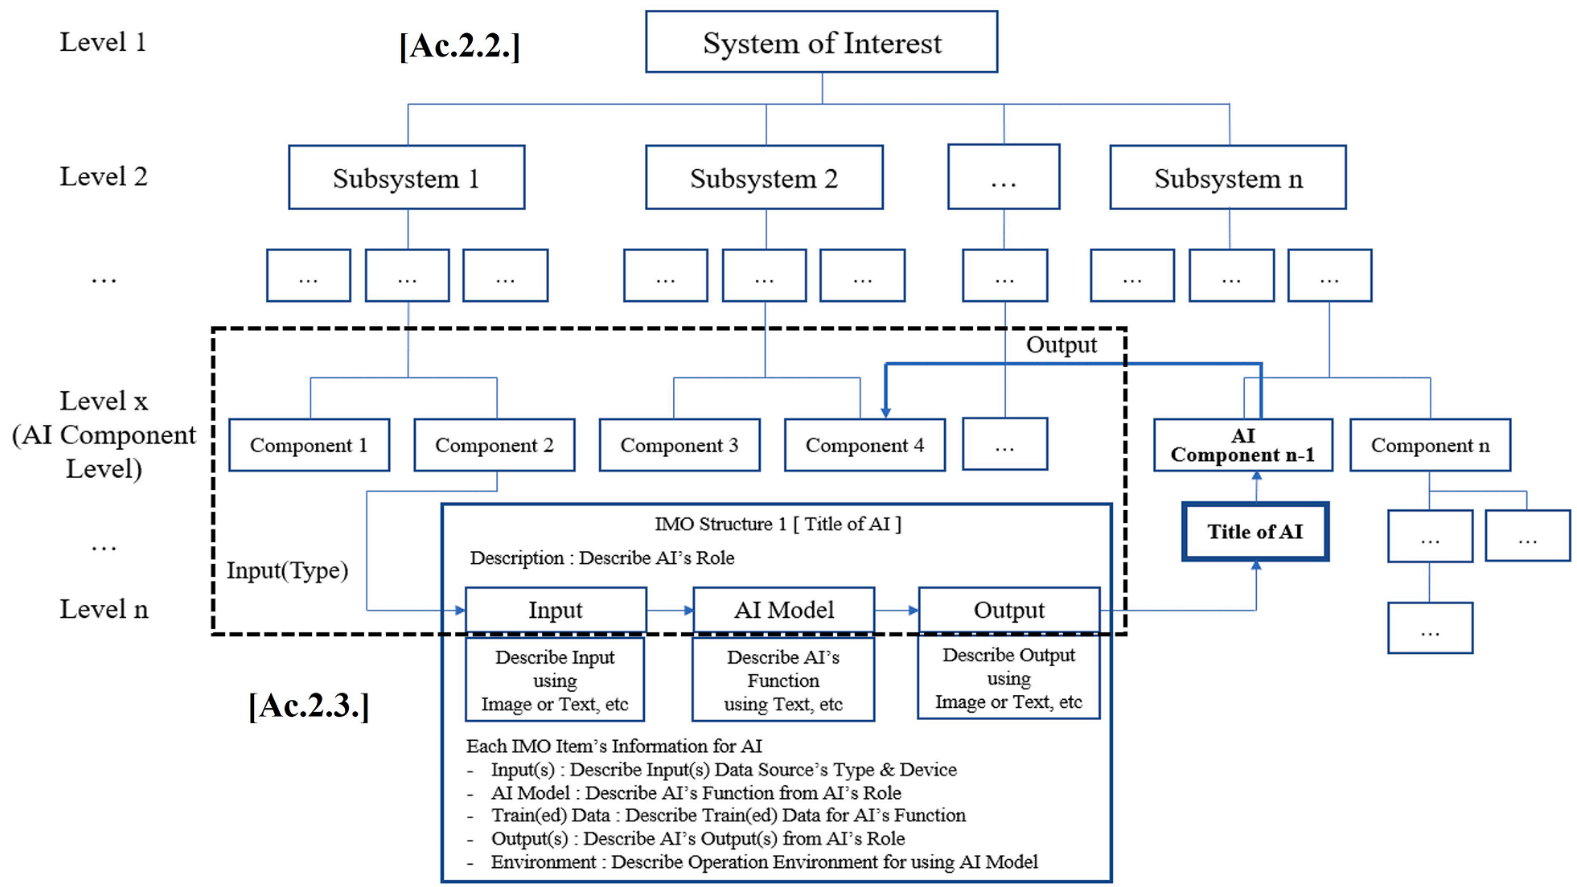
\includegraphics[width=1\linewidth]{image/fig table 2.png} \\

                            \specialrule{0.5pt}{1pt}{5pt}
                            \multicolumn{1}{c}{مولفه(های) هوش مصنوعی مورد نیاز(ها) [Ac.4.2.]} \\
                            \specialrule{0.5pt}{1pt}{1pt}
                            
                            توضیحات: نیاز(های) سطح سیستم را برای اجرای مدل هوش مصنوعی شرح دهید. \\
                            
                            \specialrule{1pt}{1pt}{1pt}
                            
                        \end{tabularx}
                        
                    \end{table}

                    \begin{table}[htbp]

                        \centering
                        \caption{خروجی اصلی در مرحله راه حل فنی هوش مصنوعی}
                        \begin{tabularx}{\textwidth}{c c c c X}

                            \vspace{-10pt}\\

                            \hline

                            \multicolumn{5}{c}{نقش هوش مصنوعی [Ac.4.3.]}\\
                            
                            \hline

                            \multicolumn{5}{c}{راه حل داده}\\

                            \multicolumn{1}{c}{I} & \multicolumn{1}{r}{ورودی} & \multicolumn{1}{r}{نوع} &  & نوع اقلام منبع ورودی را شرح دهید. (به طور مثال: تصویر، سیگنال) \\
                            & \multicolumn{1}{r}{منبع} & \multicolumn{1}{r}{صفت} &  & اطلاعات دقیقی که منبع ورودی را نشان می دهد را شرح دهید. (به عنوان مثال: وضوح، نرخ تجدید، \dots) \\
                            & \multicolumn{1}{r}{داده/محیط} & \multicolumn{1}{r}{صفت} & \multicolumn{1}{r}{نوع، میزان} & نوع و مقدار داده (یا محیط) مورد نیاز را شرح دهید. \\
                            & \multicolumn{1}{r}{نیازمندی‌ها} &  & \multicolumn{1}{r}{شرایط تفصیلی} & شرایط مورد نیازی که باید در داده ها (یا محیط) گنجانده شود را شرح دهید. (به عنوان مثال: عوامل محیطی شناسایی شده در (OV \\
                            & \multicolumn{1}{r}{بنیاد و پایه} & \multicolumn{1}{r}{منبع ورودی} &  & دلیل انتخاب عنصر I را شرح دهید. \\
                            &  & \multicolumn{2}{r}{نیازمندی‌های داده/محیط} & دلیل انتخاب الزامات عنصر I را شرح دهید. \\

                            \multicolumn{5}{c}{راه حل تکنیک هوش مصنوعی}\\

                            \multicolumn{1}{c}{M} & \multicolumn{1}{r}{مدل هوش مصنوعی} & \multicolumn{2}{c}{نوع} & انواع الگوریتم های هوش مصنوعی را توضیح دهید. (به عنوان مثال: طبقه بندی، پیش بینی) \\
                            &  & \multicolumn{2}{c}{الگوریتم} & عنوانی را که نشان دهنده الگوریتم هوش مصنوعی است توضیح دهید. \\
                            &  & \multicolumn{1}{r}{محیط} & \multicolumn{1}{r}{DEV} & محیط توسعه برای دستیابی به مدل هوش مصنوعی را شرح دهید. \\
                            &  &  & \multicolumn{1}{r}{OPS} & محیط مورد نیاز برای اجرای مدل هوش مصنوعی بدست آمده را شرح دهید. \\
                            & \multicolumn{1}{r}{بنیاد و پایه} & \multicolumn{3}{r}{دلیل انتخاب عنصر M را شرح دهید.} \\

                            \multicolumn{1}{c}{O} & \multicolumn{1}{r}{خروجی} & \multicolumn{3}{r}{شکل یا محتوای مقادیر خروجی مدل هوش مصنوعی را شرح دهید.} \\
                            & \multicolumn{1}{r}{عملکرد هوش مصنوعی} & \multicolumn{3}{r}{الزامات عملکرد مدل هوش مصنوعی را با اندازه‌گیری‌ها (یا معیارهای) مناسب توصیف کنید.} \\
                            & \multicolumn{1}{r}{نیازمندی‌ها} &  &  &  \\
                            & \multicolumn{1}{r}{بنیاد و پایه} & \multicolumn{1}{r}{خروجی} &  & \multicolumn{1}{r}{دلیل انتخاب خروجی را شرح دهید.} \\
                            &  & \multicolumn{2}{r}{عملکرد هوش مصنوعی} & \multicolumn{1}{r}{دلیل انتخاب عملکرد هوش مصنوعی را شرح دهید.} \\
                            
                            \multicolumn{2}{c}{دلیل نقش هوش مصنوعی} & \multicolumn{3}{r}{\multirow{2}{*}{توضیح دهید که چگونه ساختار کاملاً طراحی شده IMO در نهایت به نقش هوش مصنوعی دست می یابد.}} \\
                            \multicolumn{2}{c}{در سیستم مورد علاقه} & \\

                            \hline

                        \end{tabularx}
                        
                    \end{table}

                    جعبه ساختار IMO که در جدول 2 در بخش راه‌حل سیستم هوش مصنوعی ارائه شده، به طور خلاصه اطلاعات مرتبط با هر عنصر IMO را بیان می‌کند که از طریق فعالیت‌های طراحی [Ac.2.2] $\sim$ [Ac.4.2.] واقعیت‌پذیر می‌شوند. این روش نمایش برای افزایش صرافت و قابلیت استفاده معماری طراحی شده استفاده می‌شود.

                    \paragraph{3.2.2.3.}{مرحله راه حل فنی هوش مصنوعی Ac.3}

                    مرحله راه‌حل فناوری هوش مصنوعی، موارد فنی هوش مصنوعی را شناسایی یا طراحی می‌کند تا نقش هوش مصنوعی که در مرحله تعریف مسئله شناسایی شده است، دست‌یابی شود. جنبه کلیدی این مرحله تبدیل انتظارات سهام‌داران به منظر فناوری هوش مصنوعی است. برای دست‌یابی به این هدف، این مرحله از طریق همکاری با کارشناسان هوش مصنوعی و همچنین کارشناسان حوزه و سیستم انجام می‌شود. در بسیاری از مطالعات، تعریف نیازمندی‌ها برای سیستم‌های هوش مصنوعی به عنوان یک مسئله دشوار شناخته شده است [6،31]. به عنوان مثال، تعریف «عابر پیاده» که خودروهای خودران باید از آن‌ها جلوگیری کنند، چیست؟ چه «تهدیدی» باید پهپادهای بدون سرنشین در حوزه دفاع شناسایی کنند؟ در مرحله راه‌حل فناوری هوش مصنوعی، این مشکلات از طریق فعالیت‌های طراحی معماری همکارانه میان کارشناسان آدرس داده می‌شوند. نتایج فعالیت‌های طراحی، موارد فنی ناشی از ساختار IMO برای ویژگی‌های هوش مصنوعی مورد نیاز هستند. این می‌تواند تأیید کند که مسئله در حوزه دامنه به طور واضح به نیازمندی‌های فناوری هوش مصنوعی ترجمه شده است. مرحله راه‌حل فناوری هوش مصنوعی از طریق چهار فعالیت به عنوان شکل 8 زیر نشان داده شده است. به عنوان اینکه این مرحله یک فرآیند متمایز از مطالعات طراحی معماری موجود است، توضیحات تصویری اضافی برای این مرحله را اضافه کرده‌ایم تا درک را آسان‌تر کنیم.

                    \begin{figure}[htbp]

                        \centering
                        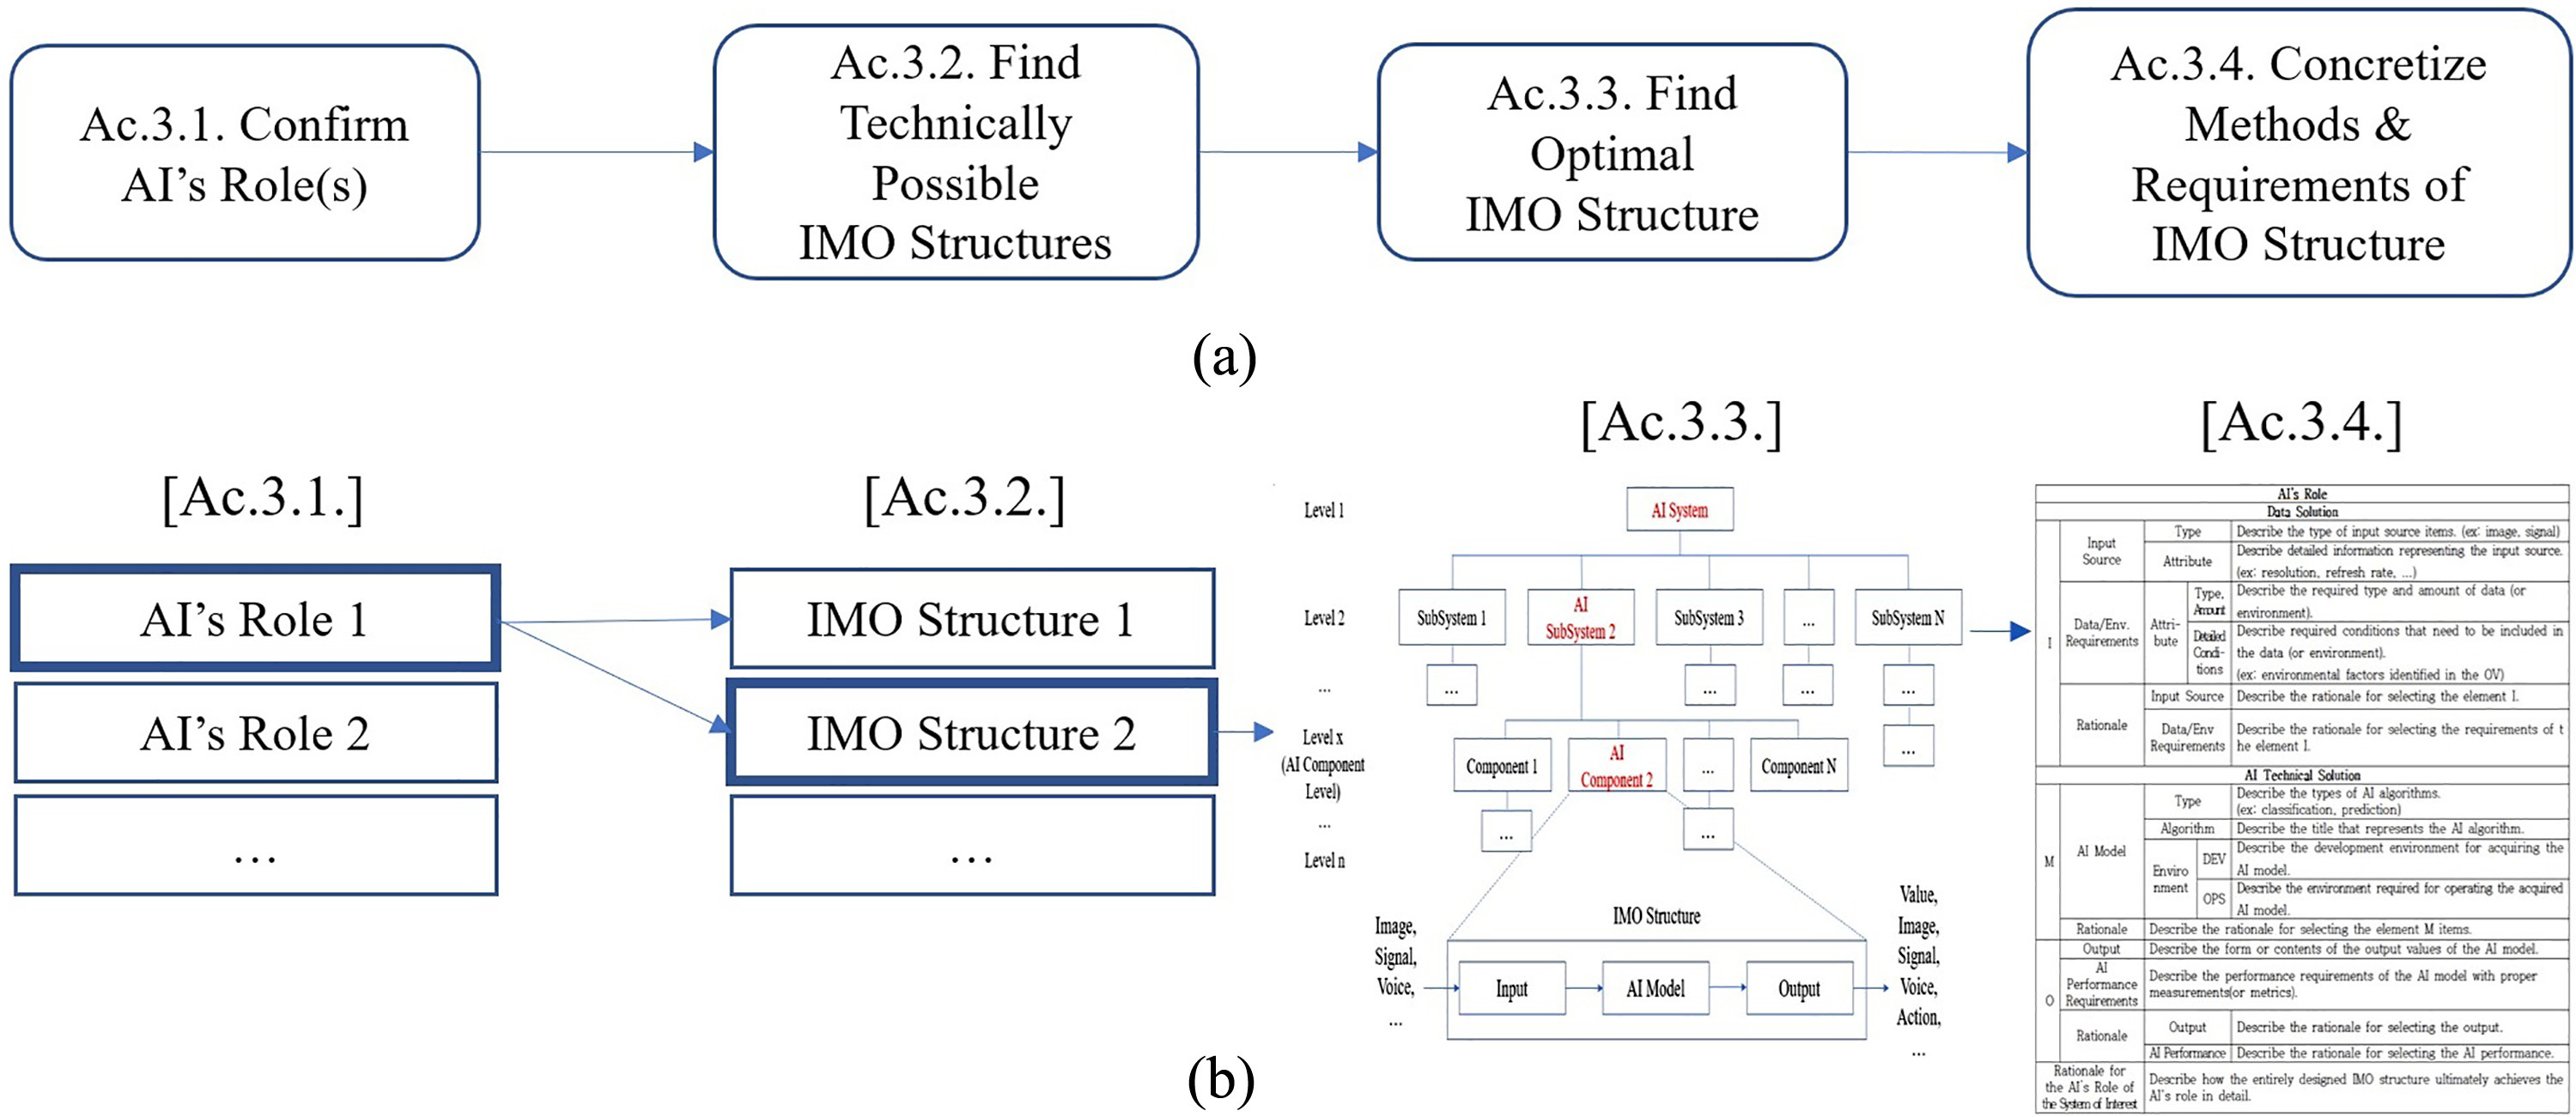
\includegraphics[width=0.8\textwidth]{image/fig 8.png}
                        \caption{الف) چهار فعالیت در مرحله حل فنی هوش مصنوعی ب) شرح گرافیکی مرحله راه حل فنی هوش مصنوعی.}
                        \label{fig:fig_8}
                    
                    \end{figure}

                    جدول 3 خروجی‌های اصلی را که در مرحله راه‌حل فناوری هوش مصنوعی باید شناسایی شوند نشان می‌دهد. توضیحات دقیق هر فعالیت که خروجی‌های اصلی را واقعیت‌پذیر می‌کنند، به شرح زیر است.

                    در فعالیت اول، نقش هوش مصنوعی که در مرحله تعریف مسئله شناسایی شده است، تأیید می‌شود. نقش هوش مصنوعی نمایانگر انتظارات سهام‌داران در مورد هوش مصنوعی در سیستم است، و این اهدافی هستند که کارشناسان هوش مصنوعی باید از طریق طراحی ساختار IMO به دست آورند (ارجاع داده شود به شکل ۸.ب [Ac.1.3.]( در فعالیت دوم، ساختارهای IMO فنی بررسی می‌شوند. حتی برای یک ویژگی هوش مصنوعی، ممکن است برای انجام آن از منظر فنی بسیاری از نامزدهای IMO وجود داشته باشد. به عنوان مثال، برای ویژگی هوش مصنوعی مانند «تشخیص اشیا»، نامزدهای فنی مختلفی مانند Yolo [23] و Faster R-CNN [49] وجود دارد (ارجاع داده شود به شکل ۸.ب [Ac.2.3.]( در فعالیت سوم، ساختار مناسب IMO از میان ساختارهای IMO فنی قابل انجام انتخاب می‌شود. انتخاب ساختار مناسب IMO همزمان با فرآیند طراحی اجزای سیستم و ساختارهای IMO در مراحل Ac.2.2 و Ac.3.2 مرحله راه‌حل سیستم هوش مصنوعی انجام می‌شود. کارشناسان هوش مصنوعی باید ساختارهای مناسب IMO را طراحی کنند، و کارشناسان سیستم باید محدودیت‌های سیستمی مانند اندازه و هزینه را در نظر بگیرند تا ساختارهای IMO را در سیستم طراحی کنند. به عنوان مثال، اجزای مختلف سیستم مانند دوربین‌های ویدئو، لیدارها و رادارها می‌توانند به عنوان عنصر I در یک سیستم خودروهای خودران در نظر گرفته شوند. انتخاب این اجزا سیستم می‌تواند بر داده‌های مورد نیاز یا عملکرد قابل دسترسی تأثیر بگذارد. علاوه بر این، از آنجا که اجزا زیادی از سیستم مورد نیاز است، اندازه یا هزینه تولید سیستم ممکن است افزایش یابد. بنابراین، تحلیل تعادل‌ها توسط کارشناسان فناوری هوش مصنوعی و جنبه‌های سیستمی از طریق همکاری و انتخاب ساختار مناسب IMO (ارجاع داده شود به شکل ۸.ب [Ac.3.3.]( در فعالیت نهایی، روش‌ها و نیازمندی‌های فنی جزئی برای پیاده‌سازی نقش هوش مصنوعی از طریق ساختار IMO که از نظر فناوری هوش مصنوعی و جنبه‌های سیستمی مشخص شده است، طراحی می‌شود. نتایج طراحی در این فعالیت مربوط به داده‌ها یا محیط، الگوریتم‌های هوش مصنوعی و خروجی‌ها، عملکرد هوش مصنوعی و نیازمندی‌های مربوط به اجزای هوش مصنوعی که در بخش 3.3.1.3 توصیف شده است، است. این‌ها بر اساس سناریوهای عملیاتی «می‌خواهیم» طراحی شده‌اند که می‌توانند انتظارات سهام‌داران را برآورده کنند. داده بر اساس مقدار و کیفیت لازم داده‌ها، روش‌های برچسب‌گذاری و غیره طراحی می‌شود، با در نظر گرفتن شرایط سناریوهای عملیاتی و اجزای سیستم. الگوریتم‌های هوش مصنوعی با در نظر گرفتن توابع مورد نیاز در نقش هوش مصنوعی طراحی می‌شوند. الگوریتم‌های هوش مصنوعی برای ایجاد مدل‌های هوش مصنوعی استفاده می‌شوند، و از آنجا که محیط‌های تهیه و عملیاتی مدل‌های هوش مصنوعی متفاوت است، همانطور که در بخش 1.3.1.3 شرح داده شده است، برای هر محیط به صورت واضح متمایز و نمایان شده‌اند تا برای استفاده بهینه از معماری در آینده قابل استفاده باشند. خروجی و عملکرد هوش مصنوعی نشانگر عملیاتی است که مدل هوش مصنوعی واقعی انجام می‌دهد، و اهمیت طراحی روشن آن برای طراحی و پیاده‌سازی یک سیستم هوش مصنوعی قابل اعتماد است. عملکرد فناوری هوش مصنوعی از طریق داده و الگوریتم‌های هوش مصنوعی تعیین می‌شود. فرض کنید که طراحی برای مقدار و کیفیت داده‌ها به درستی انجام شده باشد، متغیر باقی‌مانده روش اندازه‌گیری عملکرد برای فناوری هوش مصنوعی است. در این مقاله، تمام فناوری‌ها و روش‌های اندازه‌گیری عملکرد مربوط به یادگیری نظارت شده، یادگیری بدون نظارت و یادگیری تقویتی به منظور اهداف تحقیقاتی نمی‌شمرده شده‌اند، اما مطالعه در [58] می‌تواند به عنوان یک مرجع خوب برای طبقه‌بندی فناوری‌های هوش مصنوعی مورد استفاده قرار گیرد. فناوری‌های هوش مصنوعی در اصل احتمالاتی هستند، و بسته به نوع فناوری هوش مصنوعی استفاده شده یا زمینه استفاده از فناوری هوش مصنوعی، ممکن است روش‌های مختلفی برای اندازه‌گیری عملکرد وجود داشته باشد [23]، [24]، [25]، [26]، [27]، [28]. بنابراین، یک نکته اساسی در زمان طراحی عملکرد فناوری هوش مصنوعی، واقع‌گرایی روش‌های اندازه‌گیری عملکرد است که در نهایت انتظارات سهام‌داران را از طریق بحث و توافق به صورت واضح برآورده کنند. روش‌هایی که می‌توان مدنظر قرار داد به بخش 3.3.1.3 یا می‌توان به مورد مطالعه مانند [48] مراجعه کرد. همچنین، در فعالیت نهایی، ملاحظات فنی مربوط به ساختار IMO، که بر اساس بحث و توافق هر کارشناس حوزه از طریق هر فعالیت مرحله راه‌حل فناوری هوش مصنوعی بررسی شده‌اند، به همراه منطق آن‌ها (ارجاع داده شود به شکل ۸.ب [Ac.4.3.] و جدول 3) مشخص می‌شوند.

    % MARK: Shara
                    
    \section{نمونه موردی و تحلیل اثربخشی}

        در این مطالعه، یک روش‌شناسی برای طراحی معماری سیستم‌های هوش مصنوعی که سازمان‌ها به آن‌ها نیاز دارند، از طریق ساختار IMO شرح داده شده است. روش‌شناسی ما سیستم‌های هوش مصنوعی مورد نیاز و فناوری‌های هوش مصنوعی مورد نیاز را بر اساس فعالیت‌های عملیاتی آینده که توسط سازمان تصور می‌شود، طراحی می‌کند. علاوه بر این، مفهوم ساختار IMO را معرفی کرده‌ایم تا نیازمندی‌های فنی برای توسعه مدل‌های هوش مصنوعی مورد نیاز را شناسایی کند. به عبارت دیگر، روش‌شناسی ما محدودیت‌های مطالعات موجود که فقط نیازمندی‌های سطح انتزاعی را شناسایی می‌کنند را برطرف می‌کند و می‌تواند طراحی را با نیازمندی‌های خاص برای توسعه مدل‌های هوش مصنوعی به صورت عملی مشخص کند. در این بخش، با استفاده از روش‌شناسی ما، مطالعات موردی را توضیح داده و کارایی آن را ارزیابی می‌کنیم.

        \subsection{مورد نمونه}

            به عنوان یک نمونه از روش پیشنهادی، ما یک مثال موردی از یک سیستم ایمنی خودران برای یک وسیله نقلیه مجهز به دو وظیفه هوش مصنوعی ارائه می‌دهیم: جلوگیری از خواب آلودگی راننده و رانندگی خودکار. نتایج نمایش داده شده از طریق خروجی‌های اصلی سه مرحله از روش پیشنهادی ما است: تعریف مسئله (ارجاع داده شود به جدول 4)، راه‌حل سیستم هوش مصنوعی (ارجاع داده شود به جدول 5)، و راه‌حل فنی هوش مصنوعی (ارجاع داده شود به جدول‌های 6 و 7).

            \begin{table}[htbp]

                \centering
                \caption{خروجی اصلی مرحله تعریف مشکل برای سیستم پشتیبانی رانندگی ایمن خودمختار برای وسیله نقلیه}
                \begin{tabularx}{\textwidth}{X}

                    \hline

                    تعریف مسئله \\

                    \hline

                    [صورت مسئله] \\

                    تصادفات رانندگی ناشی از خواب آلودگی هر سال افزایش می‌یابد، و تحلیل روندهای مصرف‌کننده نشان می‌دهد که ترجیح برای خودروهای ایمن در حال افزایش است. در صنعت خودروی آینده به دلیل توسعه فناوری هوش مصنوعی، و به ویژه انتظارات مصرف‌کنندگان با تجربه رانندگی کافی که در افزایش است، تقاضا برای فناوری رانندگی خودکار در آینده در حال افزایش است. \\

                    [مشکل باید حل شود] \\

                    یک سیستم ایمنی خودکار که می‌تواند رانندگی ایمن برای رانندگان با تجربه کافی نداشته و از رانندگی در حالت خواب‌آلودگی جلوگیری کند، برای نجات یک راننده از تصادفات خودرو لازم است. \\

                    \hline

                    سناریو(ها) همانطور که هست \\

                    \hline

                    راننده برای سفر به مقصد «A» وارد خودرو می‌شود و با کنترل شخصی خودرو، از طریق جاده‌های شهری عمومی و کوچه‌ها رانندگی می‌کند. راننده به طرف جلو نگاه می‌کند و فاصله‌ای ایمن از خودروهای اطراف و عابران پیاده را حفظ می‌کند تا از وقوع حوادث جلوگیری کند. \\  

                    شرایط $\leftarrow$ زمان $\leftarrow$ روز/شب (24 ساعته) \\
                    \hspace{24pt} $\leftarrow$ فضا $\leftarrow$ شهر خیابان/اتوبان \\
                    \hspace{24pt} $\leftarrow$ دیگر $\leftarrow$ باران (با بارش 100 میلی‌متر)، برف (با بارش 50 میلی‌متر) \\

                    \hline
                    
                    سناریو(های) آینده \\

                    \hline

                    راننده برای سفر به مقصد «A» وارد خودرو می‌شود و با کنترل شخصی خودرو، از طریق جاده‌های شهری عمومی و کوچه‌ها رانندگی می‌کند. هنگامی که راننده حالت ایمنی خودرو را فعال می‌کند، خودرو به صورت خودکار حرکات جلوگیری از برخورد را در برابر خودروهای اطراف انجام می‌دهد اگر به آن‌ها نزدیکتر باشند. و هنگامی که خواب‌آلودگی راننده در حالت رانندگی تشخیص داده می‌شود، سیگنال‌های هشدار خواب‌آلودگی بر روی شیشه جلویی خودرو تولید می‌شود و لرزش‌های فرمان تولید می‌شود تا از وقوع تصادفات رانندگی ناشی از خواب‌آلودگی جلوگیری شود. \\

                    شرایط $\leftarrow$ زمان $\leftarrow$ روز/شب (24 ساعته) \\
                    \hspace{24pt} $\leftarrow$ فضا $\leftarrow$ شهر خیابان/اتوبان \\
                    \hspace{24pt} $\leftarrow$ دیگر $\leftarrow$ باران (با بارش 100 میلی‌متر)، برف (با بارش 50 میلی‌متر) \\

                    \hline

                    نقش(های) هوش مصنوعی \\

                    \hline

                    \vspace{-10pt}

                    \begin{enumerate}
                        
                        \item هنگامی که موتور روشن است و خواب‌آلودگی راننده تشخیص داده می‌شود (اگر چشمان بیش از 2 ثانیه بسته باشند)، هوش مصنوعی سیگنال‌های هشداری را به شیشه جلویی و فرمان ماشین می‌فرستد.

                        \item وقتی راننده حالت ایمن را فعال می‌کند، سپس هوش مصنوعی موقعیت خودروهای اطراف را تشخیص می‌دهد و کنترل خودرو را برای جلوگیری از برخورد کنترل می‌کند.

                    \end{enumerate}

                    \hrule

                \end{tabularx}
                
            \end{table}

            \begin{table}[htbp]
                
                \centering
                \caption{خروجی اصلی مرحله راه حل هوش مصنوعی سیستم برای سیستم پشتیبانی رانندگی ایمن خودمختار برای وسیله نقلیه}

                \vspace{-5pt}

                \begin{tabularx}{\textwidth}{ X }
                    
                    \hrule

                    ماموریت(های) سیستم هوش مصنوعی 

                    \vspace{3pt}
                    
                    \hrule

                    \vspace{3pt}

                    سیستم پشتیبانی رانندگی ایمن خودرو از رانندگی خواب‌آلود و تصادف خودرو جلوگیری می‌کند. 

                    \vspace{3pt}

                    \hrule

                    \vspace{3pt}

                    راه‌حل(های) سیستم هوش مصنوعی 

                    \vspace{3pt}

                    \hrule

                    \vspace{3pt}

                    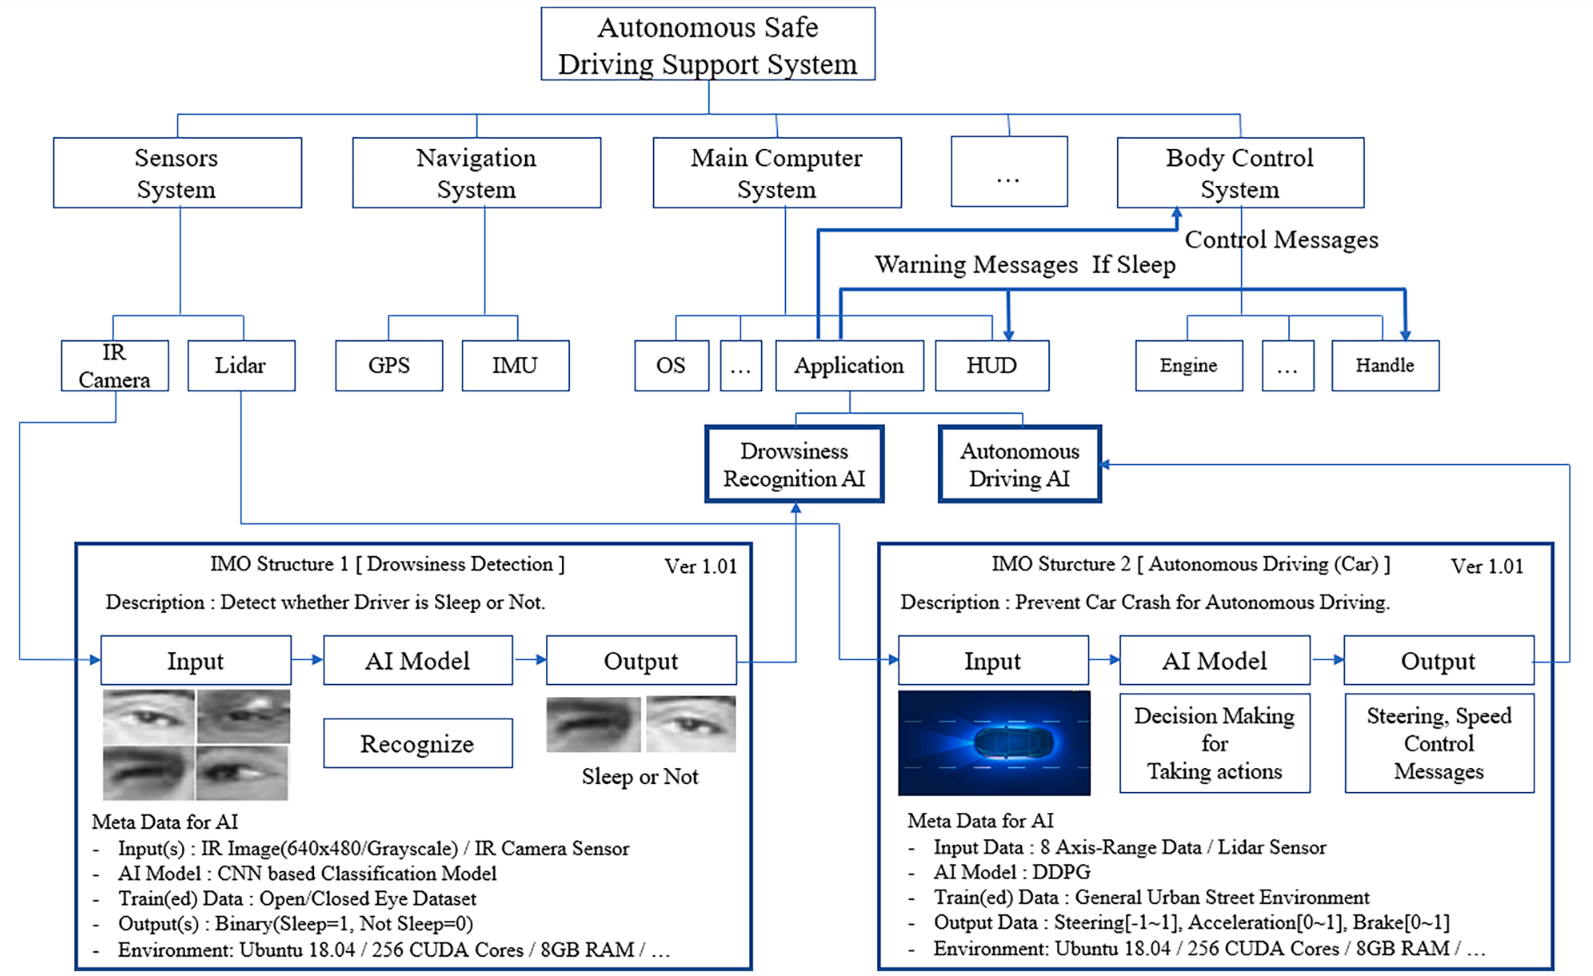
\includegraphics[width=1\linewidth]{image/fig table 5.png} 

                    \vspace{3pt}

                    \hrule

                    \vspace{3pt}

                    نیازمندی(های) مولفه(های) هوش مصنوعی

                    \vspace{3pt}

                    \hrule

                    \vspace{3pt}

                    جز اصلی سیستم کامپیوتری \\

                    \vspace{-10pt}

                    \begin{itemize}
                        
                        \item سیستم‌عامل: 04.18 Ubuntu
                        
                        \item کارت گرافیک: cores CUDA 256
                        
                        \item RAM: 8 گیگابایت
                        
                        \item حافظه: 16 گیگابایت

                    \end{itemize}

                    \hrule

                \end{tabularx}

            \end{table}

            \begin{table}[htbp]

                \centering
                \caption{خروجی اصلی مرحله راه حل فنی هوش مصنوعی برای سیستم پشتیبانی رانندگی ایمن خودمختار برای وسیله نقلیه (هوش مصنوعی تشخیص خواب آلودگی)}
                \begin{tabularx}{\textwidth}{c c c c X}

                    \vspace{-10pt}\\

                    \hline

                    \multicolumn{5}{c}{نقش هوش مصنوعی 1 (هوش مصنوعی تشخیص خواب آلودگی)}\\
                    
                    \hline

                    \multicolumn{5}{c}{راه حل داده}\\

                    \multicolumn{1}{c}{I} & \multicolumn{1}{r}{ورودی} & \multicolumn{1}{r}{نوع} &  & تصویر (دوربین مادون قرمز) \\
                    & \multicolumn{1}{r}{منبع} & \multicolumn{1}{r}{صفت} &  & 640 $\times$ 480 ، مقیاس خاکستری ، 256 رنگ (قرمز-سبز-آبی) ، 30 فریم بر ثانیه \\
                    & \multicolumn{1}{r}{داده/محیط} & \multicolumn{1}{r}{صفت} & \multicolumn{1}{r}{نوع، میزان} & تصویر چشم باز به میزان 5000 عدد، تصویر چشم بسته به میزان 5000 عدد \\
                    & \multicolumn{1}{r}{نیازمندی‌ها} &  & \multicolumn{1}{r}{شرایط تفصیلی} & شامل داده هر رنگ پوستی(سفید 33/3\% ، زرد 33/3\% ، سیاه 33/3\%) شامل 50\% داده دارای پوشش عینک (عینک طبی 25\% ، عینک آفتابی 25\%) \\
                    & \multicolumn{1}{r}{بنیاد و پایه} & \multicolumn{1}{r}{منبع ورودی} &  & برای دستیابی به نقش هوش مصنوعی، یک سنسور دوربین مادون قرمز و داده های آن که می تواند راننده را در روز/شب در داخل وسیله نقلیه زیر نظر داشته باشد و حتی با یک سنسور به عملکرد دست پیدا کند، مناسب است. \\
                    &  & \multicolumn{2}{r}{نیازمندی‌های داده/محیط} & داده‌های مورد نیاز برای یادگیری ویژگی‌ها از ویژگی های مختلف راننده (رنگ پوست، عینک زدن، \dots) تنظیم شده است. \\

                    \multicolumn{5}{c}{راه حل تکنیک هوش مصنوعی}\\

                    \multicolumn{1}{c}{M} & \multicolumn{1}{r}{مدل هوش مصنوعی} & \multicolumn{2}{c}{نوع} & تشخیص خواب آلودگی \\
                    &  & \multicolumn{2}{c}{الگوریتم} & مدل طبقه بندی مبتنی بر CNN \\
                    &  & \multicolumn{1}{r}{محیط} & \multicolumn{1}{r}{DEV} & 04.18 Ubuntu / 0.5.2 Tensorflow / 7.3 Python / \dots \\
                    &  &  & \multicolumn{1}{r}{OPS} & 04.18 Ubuntu / cores CUDA 256 / 8 گیگابایت RAM / \dots \\
                    & \multicolumn{1}{r}{بنیاد و پایه} &  &  & برای دستیابی به نقش هوش مصنوعی، لازم است یک مدل تشخیص برای تشخیص باز یا بسته بودن چشمان راننده اعمال شود. در مقایسه با الگوریتم های مشابه مانند Yolo [23]، یک مدل سبک وزن مبتنی بر CNN که می تواند توابع تشخیص را با محاسبات کم انجام دهد مناسب است. \\

                    \multicolumn{1}{c}{O} & \multicolumn{1}{r}{خروجی} & \multicolumn{3}{r}{چشم بسته(1)/باز(0)} \\
                    & \multicolumn{1}{r}{عملکرد هوش مصنوعی} & \multicolumn{3}{r}{دقت طبقه‌بندی چشم باز/بسته بیش از 95\%} \\
                    & \multicolumn{1}{r}{نیازمندی‌ها} &  &  &  \\
                    & \multicolumn{1}{r}{بنیاد و پایه} & \multicolumn{1}{r}{خروجی} &  & برای دستیابی به نقش هوش مصنوعی، لازم است نتایج شناسایی شده ارائه شود، چه چشمان راننده باز یا بسته باشد. \\
                    &  & \multicolumn{2}{r}{عملکرد هوش مصنوعی} & با توجه به اهمیت نقش هوش مصنوعی، عملکرد هوش مصنوعی باید تا حد امکان بالا باشد و با توجه به بلوغ تکنولوژیکی الگوریتم‌های مشابه روی بیش از 95\% تنظیم شود [41]. \\
                    
                    \multicolumn{2}{c}{دلیل نقش هوش مصنوعی} & \multicolumn{3}{r}{نقش 1 هوش مصنوعی که در مرحله تعریف مشکل شناسایی شده است، تشخیص خواب آلودگی راننده و} \\
                    \multicolumn{2}{c}{در سیستم مورد علاقه} & \multicolumn{3}{r}{هشدار دادن به هنگام شناسایی خواب آلودگی است. این نقش را می توان با استخراج موقعیت هر چشم} \\
                    \multicolumn{2}{c}{} & \multicolumn{3}{r}{از صورت راننده از طریق داده های تصویر دوربین IR و طبقه بندی چشم ها، بسته یا غیر بسته، از طریق} \\
                    \multicolumn{2}{c}{} & \multicolumn{3}{r}{ساختار توصیه شده IMO به دست آورد.} \\
                    \multicolumn{2}{c}{} & \multicolumn{3}{r}{اگر چشمان راننده بیش از 2 ثانیه بسته باشد (به عنوان مثال، در مورد دوربین 30 فریم بر ثانیه، اگر بیش از} \\
                    \multicolumn{2}{c}{} & \multicolumn{3}{r}{60 بار چشمان راننده توسط هوش مصنوعی «بسته» تشخیص داده شود)، به عنوان «خواب آلودگی» در نظر} \\
                    \multicolumn{2}{c}{} & \multicolumn{3}{r}{گرفته می شود. در آن زمان، مؤلفه هوش مصنوعی سیگنال‌های هشداری را به HUD واقع در شیشه جلو و} \\
                    \multicolumn{2}{c}{} & \multicolumn{3}{r}{فرمان می‌دهد.} \\

                    \hline

                \end{tabularx}
                
            \end{table}

            \begin{table}[htbp]

                \centering
                \caption{خروجی اصلی راه‌حل فنی هوش مصنوعی سیستم پشتیبانی رانندگی ایمن خودمختار برای وسیله نقلیه (هوش مصنوعی رانندگی خودکار)}
                \begin{tabularx}{\textwidth}{c c c c X}

                    \vspace{-10pt}\\

                    \hline

                    \multicolumn{5}{c}{نقش هوش مصنوعی 2 (هوش مصنوعی رانندگی خودکار)}\\
                    
                    \hline

                    \multicolumn{5}{c}{راه حل داده}\\

                    \multicolumn{1}{c}{I} & \multicolumn{1}{r}{ورودی} & \multicolumn{1}{r}{نوع} &  & داده سنسور لیدار \\
                    & \multicolumn{1}{r}{منبع} & \multicolumn{1}{r}{صفت} &  & 30 هرتز ، دامنه 0 تا 16 متر \\
                    & \multicolumn{1}{r}{داده/محیط} & \multicolumn{1}{r}{صفت} & \multicolumn{1}{r}{نوع، میزان} & محیط مجازی با قابلیت رانندگی بیش از 10000 ساعت با استفاده از حسگر لیدار - * محیط Airsim [42] بر اساس Engine Unreal [43] \\
                    & \multicolumn{1}{r}{نیازمندی‌ها} &  & \multicolumn{1}{r}{شرایط تفصیلی} & یک محیط شهری-خیابان/بزرگراه در یک محیط شهری با عابران پیاده با رفتار عادی، وسایل نقلیه اطراف، چراغ های راهنمایی و \dots و می تواند شرایط زیر را بیان کند: روز/شب (24 ساعت)، آفتابی، باران (در عرض 100 میلی متر میزان بارندگی) , برف (در عرض 50 میلی متر میزان بارش برف) \\
                    & \multicolumn{1}{r}{بنیاد و پایه} & \multicolumn{1}{r}{منبع ورودی} &  & برای دستیابی به نقش هوش مصنوعی به سنسوری با قابلیت اندازه‌گیری فاصله با دقت بالا نیاز است. از آنجایی که سنسور لیدار بهترین عملکرد را در اندازه گیری فاصله با دقت بالا در بین سایر سنسورهای موجود مانند دوربین فیلمبرداری و رادار نشان می دهد، مناسب است. \\
                    &  & \multicolumn{2}{r}{نیازمندی‌های داده/محیط} & یک محیط شهری که در آن یک راننده معمولی می‌تواند رانندگی کند، برای محیط مجازی برای یادگیری هوش مصنوعی مناسب است. \\

                    \multicolumn{5}{c}{راه حل تکنیک هوش مصنوعی}\\

                    \multicolumn{1}{c}{M} & \multicolumn{1}{r}{مدل هوش مصنوعی} & \multicolumn{2}{c}{نوع} & رانندگی خودکار (جلوگیری از تصادف خودرو) \\
                    &  & \multicolumn{2}{c}{الگوریتم} & DDPG \\
                    &  & \multicolumn{1}{r}{محیط} & \multicolumn{1}{r}{DEV} & \dots \\
                    &  &  & \multicolumn{1}{r}{OPS} & \dots \\
                    & \multicolumn{1}{r}{بنیاد و پایه} &  &  & برای دستیابی به نقش هوش مصنوعی، الگوریتم DDPG که می تواند به طور مداوم رفتار خودرو را کنترل کند، مناسب است. \\

                    \multicolumn{1}{c}{O} & \multicolumn{1}{r}{خروجی} & \multicolumn{3}{r}{فرمان [1- تا 1+] ، شتاب [0 تا 1] ، ترمز [0 تا 1]} \\
                    & \multicolumn{1}{r}{عملکرد هوش مصنوعی} & \multicolumn{3}{r}{تحت شرایط محیط مجازی مشخص شده} \\
                    & \multicolumn{1}{r}{نیازمندی‌ها} & \multicolumn{3}{r}{0\% برخورد با وسیله نقلیه یا جسم دیگر (فرد و غیره) در حین رانندگی به مدت 1000 ساعت در 10 بار} \\
                    &  & \multicolumn{3}{r}{0\% برخورد هنگام انجام موقعیت های تصادفی وسیله نقلیه و عابر پیاده به تعداد 100 بار} \\
                    &  & \multicolumn{3}{r}{(ایست ناگهانی از نزدیک وسیله نقلیه، بریدگی، عبور انسان)} \\
                    & \multicolumn{1}{r}{بنیاد و پایه} & \multicolumn{1}{r}{خروجی} &  & برای دستیابی به نقش هوش مصنوعی، هوش مصنوعی باید بتواند فرمان، پدال گاز و ترمز هر وسیله نقلیه را به طور مداوم تنظیم کند. \\
                    &  & \multicolumn{2}{r}{عملکرد هوش مصنوعی} & با توجه به اهمیت نقش هوش مصنوعی، عملکرد هوش مصنوعی باید تا حد امکان بالا باشد. برای ارزیابی ایمنی و پایداری هوش مصنوعی، شرایط رانندگی بدون تصادف به ترتیب برای 1000 ساعت در 10 بار در موارد معمول و اضطراری تنظیم شد. برای ارزیابی قابلیت واکنش اضطراری هوش مصنوعی، موقعیت‌های تصادفی تصادفی که شامل برخورد تصادفی وسیله نقلیه با وسایل نقلیه اطراف یا عابران پیاده می‌شود، 100 بار در مواقع اضطراری تنظیم شد. \\
                    
                    \multicolumn{2}{c}{دلیل نقش هوش مصنوعی} & \multicolumn{3}{r}{نقش 2 هوش مصنوعی شناسایی شده در مرحله تعریف مشکل، جلوگیری از برخورد با سایر وسایل نقلیه و} \\
                    \multicolumn{2}{c}{در سیستم مورد علاقه} & \multicolumn{3}{r}{عابران پیاده در صورت روشن بودن حالت ایمن است.} \\
                    \multicolumn{2}{c}{} & \multicolumn{3}{r}{این امر توسط هوش مصنوعی وسیله نقلیه که فاصله تا سایر اشیا اطراف خودرو را از طریق حسگر لیدار} \\
                    \multicolumn{2}{c}{} & \multicolumn{3}{r}{اندازه‌گیری می‌کند و در صورت تشخیص خطرات برخورد، فرمان و/یا سرعت خودرو را تنظیم می‌کند.} \\

                    \hline

                \end{tabularx}
                
            \end{table}

            \subsection{تحلیل اثربخشی روش پیشنهادی}

                روش پیشنهادی یک روش‌شناسی برای انجام طراحی معماری سیستم در سطح مفهومی است تا هوش مصنوعی را با موفقیت در سازمان‌ها پیاده‌سازی کند. بنابراین، انجام مقایسه عینی از اثربخشی آن آسان نیست. برای غلبه بر این مشکل، اثربخشی روش‌شناسی ما را از طریق تحلیل‌های منطقی از سه منظر ارائه می‌دهیم. اولاً، بهبودهای جزئیات روش‌شناسی خود را در مقایسه با مطالعات قبلی ارائه می‌دهیم. ثانیاً، نشان می‌دهیم که چگونه پژوهش ما می‌تواند به پیشرفت علمی در مقایسه با مطالعات در حوزه تحقیقاتی مشابه طراحی معماری سیستم کمک کند. ثالثاً، نشان می‌دهیم که روش‌شناسی ما چقدر می‌تواند احتمال موفقیت در پیاده‌سازی هوش مصنوعی در سازمان‌ها را که هدف نهایی این مطالعه است، بهبود بخشد. در نهایت، برای ارائه عینی‌تر اثربخشی روش‌شناسی خود، نتایج تحلیل و ارزیابی گروهی از کارشناسان را به صورت شفاف ارائه می‌دهیم. این گروه کارشناسی شامل پنج برنامه‌ریز و توسعه‌دهنده هوش مصنوعی بود.

                \subsubsection{تحلیل مقایسه کیفی با تحقیقات موجود}

                    در این بخش، به ارائه‌ی سهم نظری روش‌شناسی خود از طریق مقایسه‌ی کیفی موارد و نتایج تحقیقاتی موجود که برای پیاده‌سازی موفق هوش مصنوعی انجام شده‌اند، می‌پردازیم. برای تحلیل مقایسه‌ی منطقی نتایج تحقیقات، از چهار سوال Q1) تا (Q4 که در مقدمه به عنوان اهداف تحقیقاتی ارائه شده‌اند، به عنوان معیارهای ارزیابی استفاده کرده‌ایم. این سوالات نمی‌توانند به عنوان تمامی شرایط برای پیاده‌سازی موفق هوش مصنوعی در نظر گرفته شوند. زیرا طراحی سیستم‌های هوش مصنوعی برای پیاده‌سازی موفق هوش مصنوعی نیازمند نه تنها نیازهای فنی بلکه نیازهای غیرفنی مانند شفافیت، اعتمادپذیری و انصاف نیز می‌باشد [55,56]. بنابراین، چهار معیار ارزیابی برای ارزیابی و تحلیل منصفانه در چارچوب هدف و دامنه این مطالعه استفاده می‌شوند. جدول 8 زیر هر سوال و هدف آن و نتایج مقایسه منطقی بین تحقیقات موجود و روش‌شناسی ما را نشان می‌دهد.

                    \begin{table}[htbp]
                        
                        \centering
                        \caption{نتایج تحلیل مقایسه کیفی بین تحقیقات موجود و روش پیشنهادی}
                        \begin{tabularx}{\textwidth}{ c X X X }
                            
                            \hline

                            \multicolumn{1}{c}{سوالات} & \multicolumn{1}{r}{اهداف} & \multicolumn{1}{r}{مطالعات موجود} & \multicolumn{1}{r}{روش پیشنهادی} \\

                            \hline

                            \multicolumn{1}{c}{سوال 1} & شناسایی اهداف پروژه هوش مصنوعی و مفاهیم عملیاتی آینده. & مسائل یا اهمیت مربوط به محتوای هر سؤال مشخص شد، اما هیچ روش مشخصی برای پاسخ به هر سؤال ارائه نشد و رویکرد انتزاعی بود. & ارائه روش های مشخص (خروجی های اصلی مرحله تعریف مسئله) \\
                            \multicolumn{1}{c}{سوال 2} & شناسایی سیستمی که مدل هوش مصنوعی در آن مستقر خواهد شد (یا نیاز به استقرار دارد). &  & ارائه روش های مشخص (خروجی های اصلی مرحله حل هوش مصنوعی سیستم) \\
                            \multicolumn{1}{c}{سوال 3} & شناسایی الزامات فنی هوش مصنوعی مانند عملکرد و خروجی. &  & ارائه روش های ملموس (خروجی های اصلی مرحله راه حل فنی هوش مصنوعی) \\
                            \multicolumn{1}{c}{سوال 4} & شناسایی ملاحظات فنی هوش مصنوعی مانند داده ها، فناوری و غیره. &  & ارائه روش های ملموس (خروجی های اصلی مرحله راه حل فنی هوش مصنوعی) \\
                            
                            \hline

                        \end{tabularx}
                        
                    \end{table}

                    همان‌طور که در فصل ۲ شرح داده شده است، تحقیقات موجود در مورد پیاده‌سازی موفق هوش مصنوعی در سازمان‌ها از دیدگاه‌های مختلف علمی مانند قابلیت‌های سازمانی، فرآیندهای مهندسی سیستم (SE)، مهندسی نیازمندی‌ها و طراحی معماری انجام شده است. جزئیات تحقیقات موجود در فصل ۲ شرح داده شده و در اینجا حذف می‌شود. از طریق تلاش‌های بسیاری از پژوهشگران، مشخص شده است که پیاده‌سازی موفق هوش مصنوعی در سازمان‌ها نیازمند نه تنها عوامل مستقیم مرتبط با هوش مصنوعی مانند داده و فناوری، بلکه همچنین قابلیت‌های سازمانی مانند همکاری بین‌بخشی یا جذب استعدادها و عوامل محیطی می‌باشد. تحقیقات ما این پتانسیل را دارد که با پیشنهاد یک روش‌شناسی خاص برای پاسخ به چهار سوال کلیدی لازم برای پیاده‌سازی موفق هوش مصنوعی توسط سازمان‌ها، به حوزه علمی کمک کند.

                \subsubsection{مقایسه و تحلیل دیدگاه های طراحی معماری}

                    مطالعه ما از یک رویکرد مبتنی بر طراحی معماری برای پیاده‌سازی موفق هوش مصنوعی در سازمان‌ها استفاده می‌کند. برای ارزیابی اثربخشی روش‌شناسی ما، یک تحلیل مقایسه‌ای با استفاده از نتایج تحقیقات تاکدا و همکاران [16] و جولیان آی. جونز دوم و همکاران [17] که رویکردهای مشابهی با ما داشتند، انجام دادیم. معیارهای ارزیابی و محدودیت‌ها همان‌طور که در بخش 4.2.1 توصیف شده‌اند، یکسان هستند. در این بخش، ما از یک روش امتیازدهی در بازه 0 تا 2 برای مقایسه عینی در چارچوب چهار سوال ارائه شده برای هدف تحقیق استفاده کردیم. 0 امتیاز نشان می‌دهد که پاسخ قابل شناسایی نیست، 1 امتیاز نشان می‌دهد که پاسخ به صورت انتزاعی قابل شناسایی است، و 2 امتیاز نشان می‌دهد که پاسخ به صورت مشخص قابل شناسایی است. نتایج تحلیل در جدول 9 ارائه شده‌اند.

                    \begin{table}
                        
                        \centering
                        \caption{نتایج تحلیل تطبیقی از منظر طراحی معماری}
                        \begin{tabularx}{\textwidth}{ p{4cm} p{9.3cm} c c c c c }

                            \hline
                            
                            \multirow{2}{*}{کارهای مرتبط} & \multirow{2}{*}{نتجه هر مطالعه} & \multicolumn{5}{c}{امتیازات} \\
                            &  & Q1 & Q2 & Q3 & Q4 & جمع کل \\
                            
                            \hline

                            تاکدا و همکاران [16] & ارائه نتایج و روش‌شناسی طراحی معماری ربات مبتنی بر هوش مصنوعی مبتنی بر SysML & 2 & 1 & 1 & 2 & 6 \\

                            جولیان و جونز و همکاران [17] & طراحی معماری سیستم AMD مبتنی بر DoDAF و شناسایی عملکردهای هوش مصنوعی مورد نیاز & 2 & 1 & 1 & 1 & 5 \\

                            کار ما & تعریف مشکل، راه حل هوش مصنوعی سیستم، راه حل فناوری هوش مصنوعی & 2 & 2 & 2 & 2 & 8 \\

                            \hline

                        \end{tabularx}

                    \end{table}

                    اولاً، مطالعه‌ی تاکدا و همکاران [16] به طراحی و فرآیندهای عملیاتی یک ربات پشتیبانی انسانی با قابلیت‌های هوش مصنوعی داخلی با استفاده از SysML می‌پردازد. این مطالعه یک روش طراحی شفاف را ارائه می‌دهد که شامل هدف ربات، ساختار دقیق و رفتار آن بر اساس الگوریتم هوش مصنوعی داخلی، ورودی و شناسایی است. با این حال، اجزای هوش مصنوعی و مشخصات آن در سیستم ربات شناسایی نشده‌اند و مقادیر هدف عملکرد در سطح سیستم ارائه نشده است. جزء هوش مصنوعی یک عنصر طراحی حیاتی است که بر عملکرد استنتاج هوش مصنوعی و هزینه تولید سیستم تأثیر می‌گذارد. بنابراین، اگر الگوریتمی نیازمند مقدار زیادی داده‌های آموزشی و محاسبات باشد، طراحی جزء هوش مصنوعی می‌تواند ضروری در نظر گرفته شود. علاوه بر این، هدف عملکرد هوش مصنوعی داخلی در سیستم باید در مرحله طراحی بر اساس عملکرد هدف ضروری استخراج شده از مفاهیم عملیاتی آینده ارائه شود تا ریسک‌ها مانند قابلیت توسعه سیستم ارزیابی شوند.

                    مطالعه انجام‌شده توسط جولیان آی. جونز دوم و همکاران [17] نتایج طراحی معماری با استفاده از DoDAF وزارت دفاع ایالات متحده و تحلیل یک سیستم دفاع ضد موشکی (AMD) را ارائه می‌دهد. در تحقیق آن‌ها، سیستم AMD با قابلیت‌های هوش مصنوعی بیش از 17 هوش مصنوعی ضروری را از طریق طراحی OV شناسایی کرده و جریان فعالیت‌های عملیاتی و منابع را به طور دقیق شناسایی کرده است. با این حال، طراحی SV در سطح بالایی از انتزاع باقی می‌ماند و تا مرحله شناسایی اجزای هوش مصنوعی تفکیک نمی‌شود. علاوه بر این، ملاحظات فنی مانند نقش هوش مصنوعی، الگوریتم و عملکرد برای دستیابی به AI-AMD به صورت انتزاعی ارائه شده‌اند و آیتم‌های خاصی شناسایی نشده‌اند.

                    روش‌شناسی ما شامل طراحی اهداف سیستم هوش مصنوعی، مفاهیم عملیاتی، و نقش هوش مصنوعی در مرحله تعریف مسئله است. در مرحله راه‌حل سیستم هوش مصنوعی، ساختار سیستم هوش مصنوعی و طراحی اجزای هوش مصنوعی طراحی می‌شود، و در مرحله نهایی راه‌حل فنی هوش مصنوعی، نیازهای فنی برای کسب مدل‌های هوش مصنوعی طراحی می‌شود.

                \subsubsection{تحلیل اثربخشی غلبه بر علل شکست پذیرش هوش مصنوعی در سازمان‌ها}

                    این بخش اثربخشی روش‌شناسی ما را با نشان دادن این که چگونه پژوهش ما می‌تواند مشکلات شکست پذیرش هوش مصنوعی در سازمان‌های موجود را حل کند، ارائه می‌دهد. برای شناسایی علل رایج شکست پذیرش هوش مصنوعی، تحلیل‌های چندین مؤسسه پژوهشی تخصصی مانند گارتنر و مک‌کینزی را بررسی کردیم [34]، [35]، [36]، [37]، [38]، [39]، [40]. در نتیجه، شش مشکل که به طور مکرر ذکر شده‌اند را شناسایی کردیم: اهداف کسب‌وکار نامشخص، رویکرد استراتژیک نامناسب، استراتژی داده ضعیف، کمبود آگاهی از هوش مصنوعی، کمبود حکمرانی هوش مصنوعی، و کمبود استعدادهای هوش مصنوعی. برای کمّی‌سازی نتایج تحلیل خود به صورت عینی، از روشی برای اختصاص نمرات بین 0 تا 2، بسته به نتایج تحلیل برای هر علت، استفاده کردیم. در اینجا، نمره 0 نشان می‌دهد که علت حل نشده است، 1 نشان می‌دهد که حل جزئی ممکن است، و 2 نشان می‌دهد که علت می‌تواند حل شود. برای مقایسه منطقی نتایج پژوهش، هدف مقایسه نتایج تحلیل، وضعیت قبل از اعمال روش‌شناسی ما به هر علت شکست، در نظر گرفته شده و به عنوان حل نشده (0 امتیاز) ارزیابی می‌شود. جدول 10 نتایج ارزیابی برای هر علت شکست پذیرش هوش مصنوعی را نشان می‌دهد.

                    \begin{table}
                        
                        \centering
                        \caption{نتایج تحلیل بر اثربخشی غلبه بر علل شکست پذیرش هوش مصنوعی سازمانی}
                        \begin{tabularx}{\textwidth}{ p{1.5cm} p{6.5cm} c c c c p{5.5cm} }

                            \hline

                            \multicolumn{1}{c}{مشکلات} & \multicolumn{1}{c}{توضیحات} & \multicolumn{4}{c}{نتایج ارزیابی} & \multicolumn{1}{c}{بنیاد و پایه} \\
                            &  & قبل & \multicolumn{3}{c}{روش پیشنهادی} &  \\
                            &  & NS & NS & PS & S &  \\
                            &  & (0pt) & (0pt) & (1pt) & (2pt) &  \\

                            \hline

                            اهداف تجاری نامشخص & فقدان اهداف مشخص برای کسب و کارها در مورد اینکه با هوش مصنوعی چه کاری انجام دهند. & V &  &  & V & می توان با استفاده از خروجی های اصلی روش پیشنهادی بر آن غلبه کرد. \\

                            رویکرد استراتژیک نادرست & فقدان رویکردها یا فرآیندهای مناسب برای انجام پروژه های هوش مصنوعی. & V &  & V &  & امکان حل تا تحقق هدف پروژه \\

                            استراتژی داده ضعیف & عدم توانایی به دست آوردن داده های با کیفیت بالا و مقادیر زیاد مورد نیاز برای هوش مصنوعی. & V &  &  & V & می تواند از طریق خروجی اصلی مرحله 3 غلبه کند. \\

                            عدم آگاهی از هوش مصنوعی & مسائل مربوط به اعتماد به دلیل عدم آگاهی اعضای سازمان از فناوری هوش مصنوعی، مانند رد هوش مصنوعی یا اعتقاد کورکورانه به هوش مصنوعی. & V &  &  & V & اعضا می توانند هوش مصنوعی کاربردی را از طریق خروجی های اصلی روش پیشنهادی درک کنند. \\

                            فقدان حکمرانی هوش مصنوعی & عدم توانایی نظارت بر تصمیمات یا داده های هوش مصنوعی بر تصمیمات هوش مصنوعی تأثیر می گذارد. & V &  & V &  & می تواند تشخیص دهد که چه چیزی باید از طریق خروجی های اصلی روش پیشنهادی نظارت شود. \\

                            عدم استعداد هوش مصنوعی & فقدان استعداد هوش مصنوعی برای رهبری پروژه های هوش مصنوعی (از جمله هوش مصنوعی و تکنسین‌های داده) & V & V &  &  & قابل حل نیست \\

                            \hline

                            \multicolumn{2}{c}{در مجموع} & 0pt & \multicolumn{3}{c}{8pt از 12pt} \\

                            \hline

                        \end{tabularx}

                    \end{table}

                    اولین مسئله، اهداف کسب‌وکار نامشخص مشکلی است که در آن سازمان‌ها نمی‌توانند تشخیص دهند که با استفاده از هوش مصنوعی باید چه مسائلی را برای دستیابی به اهداف یا چشم‌اندازهای خود حل کنند. این مشکل را می‌توان از طریق خروجی‌های اصلی هر مرحله که در روش‌شناسی پیشنهاد شده‌اند، برطرف کرد. سناریوی عملیاتی آینده و نقش هوش مصنوعی که در مرحله تعریف مسئله شناسایی شده‌اند، در مراحل راه‌حل سیستم هوش مصنوعی و راه‌حل فنی هوش مصنوعی به طور دقیق‌تر مشخص می‌شوند. در این فرآیند، سازمان‌ها می‌توانند اهداف خود را برای چگونگی تغییر در آینده تعیین کنند و داده‌ها و فناوری‌های هوش مصنوعی مورد نیاز خود را شناسایی کنند. بنابراین، این مشکل قابل حل در نظر گرفته می‌شود.

                    دومین مسئله، رویکرد استراتژیک نامناسب به مشکلی اشاره دارد که در آن سازمان‌ها نیاز به پذیرش هوش مصنوعی را درک می‌کنند، اما نمی‌توانند آن را به پروژه‌ای با یک فرآیند روشن تبدیل کنند. این مشکل را می‌توان با اعمال روش‌شناسی پیشنهادی به مسائل کنونی یا چشم‌انداز آینده سازمان‌ها حل کرد. تصمیم‌گیرندگان درون سازمان‌ها می‌توانند از طریق خروجی‌های اصلی معماری سیستم هوش مصنوعی طراحی‌شده، پروژه را ارزیابی و تصمیم‌گیری کنند که آیا پروژه را پیش ببرند یا خیر. با این حال، دامنه روش‌شناسی پیشنهادی به فرآیند تبدیل ایده‌ها به یک مدل مفهومی قابل‌اجرا محدود می‌شود و شامل مراحل دیگر چرخه حیات توسعه مدل هوش مصنوعی، بهره‌برداری، از کار انداختن و غیره نمی‌شود. بنابراین، این مشکل به طور جزئی قابل حل در نظر گرفته می‌شود.

                    سومین مسئله، استراتژی ضعیف داده‌ها به مشکلی اشاره دارد که در آن سازمان‌ها نمی‌توانند داده‌های لازم برای هوش مصنوعی را شناسایی، جمع‌آوری و مدیریت کنند. جمع‌آوری داده‌ها به طور کلی زمان‌برترین و منابع‌برترین فرآیند در پروژه‌های هوش مصنوعی است و تأثیر قاطعی بر عملکرد هوش مصنوعی دارد. بنابراین، ایجاد یک استراتژی داده مؤثر ضروری است. این مشکل را می‌توان از طریق مرحله راه‌حل فنی هوش مصنوعی که در روش‌شناسی ما پیشنهاد شده است، حل کرد. خروجی‌های اصلی مرحله راه‌حل فنی هوش مصنوعی شامل جزئیات و دلایل مرتبط با داده‌ها و فناوری هوش مصنوعی لازم برای دستیابی به اهداف آینده سازمان است. این امر به سازمان‌ها امکان می‌دهد داده‌های واقعی مورد نیاز برای پذیرش هوش مصنوعی را شناسایی کنند. علاوه بر این، در این فرآیند، استراتژی داده مؤثری را می‌توان از طریق شناسایی و به حداقل رساندن تکرار یا اتلاف منابع و تلاش‌هایی که ممکن است در طول جمع‌آوری داده‌ها رخ دهد، ایجاد کرد. روش‌شناسی ما می‌تواند به ویژه برای سازمان‌هایی با سیستم‌های هدف بزرگ و متعدد که نیاز به استقرار هوش مصنوعی دارند و بودجه‌های محدودی دارند، مانند سازمان‌های دفاعی، مؤثر باشد. بنابراین، ما این مشکل را قابل حل در نظر می‌گیریم.

                    چهارمین مسئله، فقدان آگاهی از هوش مصنوعی است که ناشی از ناآگاهی اعضای سازمان در مورد هوش مصنوعی می‌باشد. این مشکل عمدتاً به بی‌تفاوتی یا اعتماد بی‌چون و چرا به هوش مصنوعی منجر می‌شود. این مشکل را می‌توان با افشای شفاف سناریوی عملیاتی، سلسله مراتب، نقش و عملکرد سیستم هوش مصنوعی طراحی شده از طریق روش‌شناسی پیشنهادی حل کرد. این افشاگری به اعضای سازمان این امکان را می‌دهد که بفهمند چرا هوش مصنوعی ضروری است، چگونه کار می‌کند و چه عملکردها و قابلیت‌هایی دارد. بنابراین، نتیجه می‌گیریم که این مسئله قابل حل است.

                    پنجمین مسئله، کمبود حاکمیت هوش مصنوعی، به توانایی نظارت بر عملکرد هوش مصنوعی مستقر شده در اجرای وظایف مورد نظر مربوط می‌شود. برای حل این مشکل، لازم است بتوان نظارت کرد که آیا سیستم هوش مصنوعی در محدوده عملکرد طراحی‌شده در محیط مورد نظر عمل می‌کند یا خیر. خروجی‌های اصلی هر مرحله از روش‌شناسی پیشنهادی شامل جزئیات محیط عملیاتی و عملکردهای سیستم هوش مصنوعی است. بنابراین، سازمان‌ها می‌توانند از این اطلاعات برای شناسایی مواردی که باید نظارت شوند، استفاده کنند. با این حال، اگرچه روش‌شناسی پیشنهادی می‌تواند به شناسایی عناصر مورد نیاز برای نظارت بر سیستم‌های هوش مصنوعی مستقر شده کمک کند، اما نحوه نظارت بر آنها را به طور کامل پوشش نمی‌دهد. این امر به یک فرآیند نظارتی جداگانه مبتنی بر سیستم‌های ابری یا شبکه نیاز دارد. بنابراین، ما این مشکل را تا حدودی قابل حل می‌دانیم.

                    آخرین مسئله، کمبود استعدادهای هوش مصنوعی، به کمبود کارشناسان فناوری هوش مصنوعی یا داده در سازمان‌ها اشاره دارد. پذیرش هوش مصنوعی نیازمند کارشناسانی در حوزه‌های مختلف، مانند فناوری، داده، شبکه‌ها و فرآیندهای کسب‌وکار است. روش‌شناسی پیشنهادی ما فرآیندی برای طراحی معماری سیستم هوش مصنوعی از دیدگاه‌های مختلف متخصصان در عملیات، سیستم و فناوری هوش مصنوعی ارائه می‌دهد. با این حال، این روش‌شناسی در نهایت به موضوع جذب استعدادهای جدید نمی‌پردازد. بنابراین، این مشکل غیرقابل حل در نظر گرفته می‌شود. استراتژی آموزش هوش مصنوعی وزارت دفاع ایالات متحده JAIC) (DoD [18] می‌تواند مرجع خوبی برای حل مشکل کمبود استعدادهای هوش مصنوعی باشد.

                    براساس تحلیل شش مورد ذکر شده در بالا، روش ما در جنبه‌های تعیین اهداف پروژه‌های هوش مصنوعی، ایجاد استراتژی‌های مؤثر داده و بهبود آگاهی از هوش مصنوعی ارزش استفاده بالایی دارد، که بالاترین امتیازات را در میان مشکلات موجود دریافت کرده است. علاوه بر این، تأیید کرده‌ایم که می‌توانیم به‌طور جزئی مشکلات دیگر موارد را به جز کمبود استعداد هوش مصنوعی بهبود بخشیم.

                \subsubsection{ارزیابی اثربخشی و محدودیت‌ها توسط گروه متخصص}

                    روش ما یک تلاش علمی جدید با هدف پذیرش موفقیت‌آمیز هوش مصنوعی در سازمان‌ها است. بنابراین، برای ارزیابی عینی‌تر و حرفه‌ای‌تر اثربخشی و محدودیت‌ها، نتایج بررسی توسط یک گروه کارشناسی متشکل از کارشناسان خارجی را در این فصل ارائه می‌دهیم. کارشناسان خارجی که برای ارزیابی دعوت شده‌اند، افرادی هستند که در حال حاضر در توسعه نرم‌افزارهای هوش مصنوعی، برنامه‌ریزی و مدیریت پروژه‌های هوش مصنوعی مشغول به کار هستند و دانش فنی و تجربه عملی کافی در زمینه هوش مصنوعی دارند. کارشناسان خارجی که در ارزیابی شرکت کردند در جدول 11 فهرست شده‌اند.

                    \begin{table}
                        
                        \centering
                        \caption{اطلاعات کارشناسان شرکت کننده در ارزیابی}
                        \begin{tabularx}{\textwidth}{ p{4.5cm} p{5cm} p{6cm} c }
                            
                            \hline

                            \multicolumn{1}{c}{نام} & \multicolumn{1}{c}{سازمان} & \multicolumn{1}{c}{رشته تخصصی} & \multicolumn{1}{c}{دوره‌ها} \\

                            \hline

                            (P1) M.S.Yang (مهندس ارشد) & تیم نیروی دریایی Systems Hanhwa & توسعه سیستم های رزم دریایی/SW & 25+ سال \\
                            (P2) M.W.Lee (دکتری) & ROK DAPA	 & مهندسی نرم‌افزار، فرآیند اکتساب دفاعی & 10+ سال \\
                            (P3) J.H.Ahn (ارشد) & وزارت دفاع ملی ROK (تیم آماده سازی مرکز هوش مصنوعی) & برنامه ریزی، مدیریت پروژه هوش مصنوعی & 10+ سال \\
                            (P4) J.W.Uhm (دکتری) & ستاد ارتش ROK & مهندسی نرم‌افزار، فرآیند اکتساب دفاعی & 15+ سال \\
                            (P5) S.Y.Lee (دکتری) & مدیر ارشد فناوری LG الکترونیک (دفتر ارشد فناوری) & کلان داده، توسعه SW هوش تعبیه شده & 5+ سال \\

                            \hline

                        \end{tabularx}

                    \end{table}

                    بررسی توسط گروه کارشناسی توسط هر کارشناس از طریق تخصص و تجربه عملی خود انجام شد؛ او نیازمندی‌ها و ضرورت تحقیقات ما را ارزیابی کرد و اثربخشی و محدودیت‌های روش پیشنهادی را بررسی کرد. برای یک بررسی موثر، با هر کارشناس به طور جداگانه تماس گرفته شد تا محتوای خاص تحقیق و هدف ارزیابی را به وی توضیح داده شود و سپس نتایج تحقیق از طریق ایمیل ارسال شد. مدت زمان بررسی حدود 1 تا 3 هفته طول کشید. به منظور ارائه موثر نتایج بررسی هر کارشناس، ما خلاصه و توضیح محتوای اصلی دیدگاه‌ها را ارائه دادیم و برخی از دیدگاه‌های کارشناسان را به‌طور مشترک شرح دادیم.

                    P1 ارزیابی کرد که مواجهه با تحقیقات در زمینه طراحی مفهومی برای پذیرش موفق هوش مصنوعی معنادار است و ارزیابی کرد که پژوهشگران یک روش‌شناسی را به طور منطقی و به شکلی قابل اندازه‌گیری واقع بر ساختار IMO معرفی کرده‌اند. همچنین، P1 ارزیابی مثبتی از نظر پیشرفت علمی و ارزش متنوع استفاده از روش‌شناسی ارائه شده داشت، اما اشاره کرد که نیاز به تحقیقات اضافی برای به‌طور منطقی اندازه‌گیری عملکرد هوش مصنوعی وجود دارد.

                    \begin{addinfo}

                        (P1) نیازهای ذینفعان دفاعی از حوزه‌های تخصصی برخیا می‌آیند و حتی توسعه‌دهندگان نرم‌افزارهای دفاعی با تجربه مثل خودم سختی دارند که این نیازها را به طور واضح درک و به شکل مشخصی به مرحله نیازها برای مبنای گزارش‌ها برسانند. در این زمینه، همانطور که پژوهشگران اشاره کردند، من با چالش واقعیت پذیرش هوش مصنوعی موافقم. من معتقدم که یک مطالعه و آزمایش معنی‌دار و ارزشمند است که برای حل این مشکلات به طراحی مفهومی، اولین فرآیند کلیدی برای توسعه یک سیستم موفق، می‌پردازد. همچنین فکر می‌کنم استفاده از مفهوم ساختار IMO برای طراحی معماری سیستم‌های هوش مصنوعی بسیار خلاقانه و معقول است. فصل 3 مفهوم ساختار IMO را به طور واضح ارائه می‌دهد و ملاحظاتی برای طراحی سیستم‌های هوش مصنوعی را به صورت منطقی استخراج می‌کند. روش ارائه شده در فصل 4 نیز به طور بسیار محکم فرآیند طراحی سیستم‌های هوش مصنوعی مورد نیاز در آینده را نسبت به حالت کنونی از طریق مفهوم ساختار IMO که ارائه کرده‌اند، نشان می‌دهد. روش آن‌ها را در جنبه‌های زیر ارزیابی می‌کنم. اول، پیشرفت علمی. آن‌ها به صورت خلاقانه و معقول یک روش برای طراحی یک چشم‌انداز هوش مصنوعی که AF های موجود مانند DoDAF در ایالات متحده یا MNDAF در وزارت دفاع ملی کره که اصلی است، نتوانسته‌اند به شکل محکمی محکم شوند، ارائه می‌دهند. دوم، ارزش‌های مختلف روش. همانطور که در بخش بحث مطرح شده است، با طراحی یک سیستم هوش مصنوعی از زاویه‌ای مستقل که بر مدل‌های هوش مصنوعی متمرکز است، می‌توان از ضرورت‌های مهمی مانند شفافیت و قابلیت توضیح سیستم هوش مصنوعی استفاده کرد. علاوه بر این، اگرچه آن‌ها مستقیماً در این مطالعه به این موضوع پرداخته‌اند، اما می‌توان آن‌ها را هم در مشخصه‌گذاری عملکرد مدل‌های هوش مصنوعی در روش پیشنهادی‌شان ممکن است هنوز ابهام وجود داشته باشد. مثال ارائه‌شده در مقاله بسیار توصیفی است و فرآیند یافتن منطقیت نیز به طور دقیق ارائه شده است، بنابراین می‌توان آن را به عنوان یک مورد مدل تلقی کرد. با این حال، این یک مورد است که به محدودیت مورد مطالعه خود محدود است و همه انواع فناوری‌های یا سیستم‌های هوش مصنوعی را که ممکن است به شکل متنوعی وجود داشته باشند، نشان نمی‌دهد. البته، بهرحال، قابلیت ارائه‌ی همه انواع موارد کاربردی و بهترین روش‌ها از طریق روش شان و ایجاد فرآیندی برای تعریف منطقیت از طریق تحقیقات اضافی، ارزش روش آن‌ها را افزایش می‌دهد.

                    \end{addinfo}

                    P2 بیان کرد که با وجود افزایش انتظارات اعضای سازمان‌های دفاعی از هوش مصنوعی، الزامات هنوز انتزاعی هستند. روش ما به عنوان یک موضوع اصلی در حوزه مهندسی نرم‌افزار ارزش علمی دارد، که با موضوع سیستم‌های مبتنی بر هوش مصنوعی به عنوان یک مسئله اصلی، مد نظر است، زیرا مختصر و واضح است. با این حال، بیان شد که روش ما ممکن است هنوز برای الگوریتم‌های هوش مصنوعی تولیدی اظهارات مبهمی داشته باشد، و اشاره شد که نیاز به تلاش برای تکمیل آن با جمع‌آوری موارد کاربردی مختلف و بهترین روش‌ها می‌باشد.

                    \begin{addinfo}
                        
                        (P2) بسیاری از صاحبان سابقه مربوط به سازمان‌های دفاعی به نظر می‌رسد منتظر نتایجی از هوش مصنوعی باشند. با این حال، الزامات برای توسعه سیستم هنوز انتزاعی است. به عنوان مثال، نقش‌های خاصی باید "کارکنان هوش مصنوعی" چه وظایف خاصی را انجام دهند تا تصمیم‌گیری‌های نبردی را پشتیبانی کنند؟ روش پژوهشگران می‌تواند راه‌حلی مختصر و واضح باشد. اگر صاحبان سابقه دفاعی از روش پژوهشگران استفاده کنند، به آنها کمک خواهد کرد تا الزامات انتزاعی خود را مشخص کنند. (…) طراحی یک سیستم مبتنی بر هوش مصنوعی یکی از مسائل اصلی در حوزه مهندسی نرم‌افزار است. فکر می‌کنم که طراحی سیستم انجام شده در اطراف مفهوم ساختار IMO که توسط پژوهشگران پیشنهاد شده است، اصلی است و کافی ارزش دارد تا به علم کمک کند. همچنین، می‌توان آن را به عنوان یک قطعه شواهدی در نظر گرفت که نیازی به تحقیقات اجتماعی نیست که حتی فرم‌های معاملاتی مانند DODAF یا MODAF که تا کنون در زمینه تهیه و تدوین دفاعی به کار گرفته شده‌اند، دشوار است به منظور ارائه یک فرآیند مناسب یا چارچوب در نظر گرفتن ویژگی‌های سیستم‌های هوش مصنوعی. با این حال، هنوز در مرحله علمی یا آزمایشی است و نیاز به شناسایی و تکمیل نقصان از طریق برنامه‌های عملی دارد. به عنوان مثال، چگونه می‌توان الگوریتم‌های هوش مصنوعی تولیدی مانند ChatGPT را به عنوان یک خروجی اصلی از مرحله راه‌حل فنی هوش مصنوعی تعریف کرد؟ البته، من متوجه هستم که همانطور که پژوهشگران اشاره کرده‌اند، هنوز روش یا کنوانسیونی واضح در علم برای این قسمت وجود ندارد. فکر می‌کنم که اگر موارد کاربردی مختلف و بهترین روش‌ها با استفاده از تحقیقات آن‌ها جمع‌آوری شوند، ممکن است به عنوان یک کنوانسیون در علم یا صنعت به وجود آید.

                    \end{addinfo}

                    P3 توجه به این نکته که بسیاری از پروژه‌ها و کارهای تحقیقاتی مربوط به هوش مصنوعی در حوزه دفاع اغلب متوقف می‌شوند، نیاز به فرایند کاری موثر را تأکید کرد. همچنین ارزیابی شد که آن‌ها موضوعات ارزشمندی را در بخش بحث مطرح کرده‌اند و می‌توانند راه‌حل‌هایی برای مسائل کلیدی مانند شفافیت یا قابلیت توضیح سیستم‌های هوش مصنوعی دفاعی و جلوگیری از سرمایه‌گذاری تکراری منابع سازمانی ارائه دهند. با این حال، آن‌ها نیازمندی به تحقیقات اضافی در مورد اینکه چگونه می‌توان نیازمندی‌های غیر عملکردی یا استفاده تکراری از منابع مطرح شده در بخش بحث را به طور واقعی ارزیابی کرد، را ذکر کردند.

                    \begin{addinfo}
                        
                        (P3) از بودجه‌های فلکی برای توسعه سیستم‌های هوش مصنوعی دفاعی استفاده می‌شود، اما اغلب مواقع مشاهده می‌شود که به دلیل نیازهای نامشخص، در مرحله تصمیم‌گیری، پروژه‌ها متوقف می‌شوند. (...) در کره، مرکز هوش مصنوعی دفاعی به زودی تأسیس می‌شود و نیازمند یک فرایند کاری مناسب برای تعریف وضعیت آینده سیستم‌های هوش مصنوعی مورد نیاز نیروهای مسلح ما به محور مرکز هوش مصنوعی دفاعی است. سوالات Q1) تا (Q4 ارائه شده توسط پژوهشگران مناسب هستند و آن‌ها فرایند تعریف دقیق پاسخ‌ها را به طور سیستماتیک ارائه می‌دهند. من فکر می‌کنم این برای عملگران دفاعی که نیاز به تعریف دقیق نیازمندی‌های سیستم‌های هوش مصنوعی دارند، به کمک بزرگی خواهد بود. بخش بحث هم جالب است و مسائل ارزشمندی را مورد بحث قرار می‌دهد. به‌ویژه در سازمان‌های دفاعی، به دلیل نیازمندی‌های نامشخص و انتزاعی برای سیستم‌های هوش مصنوعی، احتمالاً سرمایه‌گذاری تکراری در منابع وجود دارد. وزارت دفاع ایالات متحده (DoD) که بیش از ۶۸۰ پروژه هوش مصنوعی را اجرا می‌کند، نیز از طریق سازمان‌های نظارتی مانند دفتر مسئولیت دولت (GAO) برای استفاده شفاف از بودجه‌ها پیگیری می‌شود. پروژه‌هایی که نامشخص یا به عنوان منطقی شناخته نمی‌شوند ممکن است متوقف شوند. بنابراین، موضوعاتی که آن‌ها از طریق بخش بحث در حال بررسی هستند، موضوعاتی هستند که برای پذیرش و عملکرد پایدار هوش مصنوعی در سطح سازمانی باید حتماً بررسی شود و فکر می‌کنم آن‌ها گزینه‌های مناسب و ارزشمندی را از دیدگاه نظری ارائه داده‌اند. اگرچه هنوز موردی وجود ندارد که روش پژوهشگران به پروژه‌های واقعی هوش مصنوعی اعمال شود، من فکر می‌کنم که تحلیل اثربخشی آن‌ها در محدوده پژوهش مناسب ارزیابی شده است. (...) با این حال، برای تحقق روش پژوهشگران، لازم است تحقیقات را به گسترش بخشید تا شامل کل دوره عمر مدل‌های هوش مصنوعی مانند MLOPS شود. همچنین فکر می‌کنم که نیاز به تحقیقات اضافی برای ارزیابی دقیق مشخصه‌های غیر کارکردی یا تکراری بودن سرمایه‌گذاری منابع مورد بحث در بخش بحث است.
                        
                    \end{addinfo}

                    P4 از آنجا که در محیط توسعه سیستم‌های دفاعی ویژه، با وجود افراد مختلفی دشواری‌ها وجود دارد، روش‌شناسی ما که هر چشم‌انداز را به مفهوم ساختار IMO متمرکز می‌کند، احتمال موفقیت در توسعه سیستم‌های هوش مصنوعی دفاعی را افزایش خواهد داد. همچنین، ارزیابی شد که رویکرد به کارگیری دیدگاه هوش مصنوعی به طور جداگانه می‌تواند باعث افزایش قابلیت استفاده مجدد در توسعه سیستم‌های هوش مصنوعی مشابه شود و از این طریق بهبود کارایی استفاده از منابع سازمانی را به ارمغان آورد.

                    \begin{addinfo}
                        
                        (P4) با تشخیص مساله توسط نویسندگان موافقم. ارتش جمهوری کره به طور مداوم در تلاش است تا در محیط‌های جنگی آینده که فناوری‌های جدید مانند سامانه TIGER ارتش کره 4.0 به کار رفته‌اند، مفاهیم عملیاتی و فناوری‌ها را توسعه دهد. با این حال، محیط جنگی پیچیده است و جنگ‌ها از طریق تعامل بین انواع مختلفی از سیستم‌ها انجام می‌شوند. تا به امروز، ارتباط بین فناوری هوش مصنوعی و سیستم‌ها تا حدی ناامیدکننده بوده است. مقامات نظامی که باید تصمیم بگیرند که چگونه بجنگند، هوش مصنوعی را خوب نمی‌شناسند و نمی‌توانند از نوآوری‌هایی که هوش مصنوعی می‌تواند به همراه داشته باشد، بهره ببرند، و تکنسینان هوش مصنوعی دشواری در فهمیدن مسائل در زمینه‌های تخصصی که ارتش می‌خواهد دارند. روش پیشنهادی توسط پژوهشگران می‌تواند در مرحله طراحی مفهومی کمک کند تا مفهوم عملیاتی مطلوب ما را شناسایی کند و سیستم‌ها و فناوری‌های هوش مصنوعی لازم را تشخیص دهد. به خصوص، برای توسعه سیستم مولفه‌های هوش مصنوعی جاسازی شده در یک سیستم دفاعی پیچیده، لازم است بین سیستم‌های خارجی و داخلی تمایز قائل شویم و این سیستم‌ها را از طریق تنظیم مناسب ساختار سیستم و طراحی معماری مانند EFFBDها به وضوح تعریف کنیم، و روش آن‌ها می‌تواند به عنوان یک جایگزین برای این کار استفاده شود. (...) همانطور که در بخش بحث ذکر شده است، به نظر می‌رسد که مدل‌های هوش مصنوعی که از طریق معماری طراحی شده‌اند، می‌توانند به راحتی‌ترین نحو ممکن بررسی مجدد استفاده را در نظر بگیرند و این یک مزیت مهم است که می‌تواند منجر به کاهش موثر مصرف تکراری از منابع محدود در سازمان‌های دفاعی شود.
                        
                    \end{addinfo}

                    P5 به اهمیت توضیح دادن بهتری درباره هوش مصنوعی به مشتریان به عنوان یکی از عوامل مهم برای جلوگیری از شکست به کارگیری هوش مصنوعی در شرکت‌های عمومی فناوری اطلاعات اشاره کرد و ارزیابی کرد که فعالیت طراحی فعالیت‌های عملیاتی مهندسی معکوس متداول ما ممکن است جایگزین موثری باشد. با این حال، P5 بیان کرد که روش‌شناسی ما تنها بر روی مرحله طراحی سیستم تمرکز دارد و نیاز به گسترش تحقیقات به کل دوره عمر سیستم وجود دارد.

                    \begin{addinfo}
                        
                        (P5) شناسایی نیازهای مشتریان یا کاربران پتانسیلی یکی از وظایف اصلی است که تمام سازمان‌ها با آن روبه‌رو خواهند شد. حتی اگر یک فناوری به طور نظری در یک حوزه خاص اثبات شده باشد، اجرای آن در محیط مختلف نیازمند تلاش و هزینه‌های اضافی است. این مخصوصاً برای حوزه‌های فناوری حساس به داده مانند هوش مصنوعی صادق است. (...) تحقیقات آن‌ها مناسب برای شناسایی فناوری بر اساس نیازها به جای شناسایی نیازها بر اساس فناوری تلقی می‌شود و به عنوان یک جایگزین مناسبی که با اهداف تحقیقاتی محققان همخوانی دارد، در نظر گرفته می‌شود. (...) حتی شرکت‌های فناوری اطلاعاتی که تعداد زیادی توسعه‌دهنده هوش مصنوعی دارند، از استفاده از هوش مصنوعی احتیاط می‌کنند زیرا اعتماد کور به نتایج هوش مصنوعی می‌تواند به شرکت‌ها آسیب قابل توجهی بزند. به عنوان نتیجه، مؤسسات تحقیقاتی شرکت‌های اخیراً در حال تحقیق در زمینه طراحی عملیات برای توضیح دادن هوش مصنوعی به خوبی هستند. (...) ساختار IMO که توسط نویسندگان استفاده شده است، بسیار شفاف و آسان به فهم است. بسیار قابل توجه است که آن‌ها با اتصال مراحل فعالیت‌های عملیاتی از طریق آن، یک سیستم هوش مصنوعی توسعه داده‌اند. (...) با این حال، توسعه واقعی سیستم‌ها یا خدمات هوش مصنوعی تنها به برنامه‌ریزی یا طراحی مفهومی محدود نمی‌شود. در حالی که جنبه‌های علمی و عملی کار آن‌ها می‌تواند در چارچوب تحقیقات آن‌ها شناخته شود، برای اینکه پیشنهاد آن‌ها به عنوان یک روش بهتر ایجاد شود، نیاز به گسترش تحقیقات به تمام چرخه عمر سیستم وجود دارد. من پیشنهاد می‌کنم که ارزش تحقیقات به همراه MLOPS که در بسیاری از شرکت‌ها مورد بحث قرار دارد، گسترش یابد.

                    \end{addinfo}

                    نتیجه‌گیری از بررسی جامع از طریق گروه متخصصان نشان داد که تمامی کارشناسان با مشکل پذیرش سیستم‌های هوش مصنوعی موافق بودند. آن‌ها همچنین نظر دادند که در محتوای تحلیلی از کارآمدی روش پیشنهادی ما، هیچ اغراق یا دروغی وجود ندارد. اکثریت کارشناسان ،P1) ،P2 (P5 ارزش علمی آن را تشخیص دادند، و کارشناسان باقیمانده ،P3) (P4 نیز ارزیابی کردند که روش ما می‌تواند یک جایگزین موثر برای تعریف سیستم‌های هوش مصنوعی که سازمان‌ها نیاز دارند باشد. آن‌ها همچنین اقرار کردند که بحث در فصل 5 به مسائل ارزشمندی که برای پذیرش موفق هوش مصنوعی در سازمان‌ها مطرح شده، پرداخته است ،P1) ،P3 .(P4 با این حال، محدودیت‌ها نیز ذکر شدند. آن‌ها اشاره کردند که هنوز در مرحله علمی و آزمایشی است که تاکنون بر پروژه‌های واقعی اجرا نشده است، و نیاز به ایجاد مورد استفاده‌های بیشتر یا بهترین روش‌ها ،P2) (P3 دارد. علاوه بر این، برخی از کارشناسان ارزیابی کردند که نیاز به گسترش تحقیقات به همراه MLOPS برای توسعه موفق سیستم‌های هوش مصنوعی وجود دارد ،P1) .(P5 به طور خلاصه از نظرات و ارزیابی‌های کارشناسان، تحقیقات ما می‌تواند یک راه‌حل خوب برای طراحی سیستم‌های هوش مصنوعی که سازمان‌ها نیاز دارند باشد، و عواملی که به عنوان عواملی که باید تکمیل شوند مورد اشاره قرار گرفته‌اند مانند کمبود موردهای استفاده، روش تعریف برای الگوریتم‌های هوش مصنوعی تولیدی و ارتباط با MLOPS نیازمند تکمیل روش از طریق تحقیقات آینده هستند.

    \section{بحث}

        پژوهش ما برای پاسخ به سوالات زیر انجام شد: سازمان با فناوری هوش مصنوعی چه کاری انجام می‌دهد؟ چه الزاماتی برای تهیه مدل‌های هوش مصنوعی لازم است؟ مدل‌های هوش مصنوعی باید کجا نصب شوند؟ مدل‌های هوش مصنوعی باید چه عملکردی داشته باشند؟ ما یک روش برای پاسخ به این سوالات از طریق استفاده از ساختار IMO و طراحی معماری سیستم پیدا کردیم. و ما سه نتیجه مهم را که از طریق روش ما قابل دستیابی است، شناسایی کردیم.

        اولاً، روش ما قابلیت ارائه یک رویکرد موثر برای حل مشکلات سازمانی میان کارشناسان حوزه، کارشناسان سیستم و حرفه‌ایان هوش مصنوعی را اثبات کرده است. طراحی و شناسایی الزامات برای سیستم‌های هوش مصنوعی آینده که سازمان‌ها نیاز دارند، یک وظیفه بسیار چالش‌برانگیز است. شرکت Corporation Rand آمریکا گزارش داد که 'جمع‌آوری تمام داده‌ها' به عنوان یک فلسفه برای توسعه هوش مصنوعی که در آینده در بخش تجاری نیاز است، در حال همگرایی است، و بنابراین آن‌ها ادعا کردند که نیروی هوایی آمریکا هم باید 'همه چیز را ذخیره کند' را پذیرفته [63]. بسیاری از سازمان‌ها در فرآیند ادغام هوش مصنوعی شکست می‌خورند، و برخی از مطالعات ادعا می‌کنند که روش‌های جدید برای تعریف یا شناسایی الزامات سیستم‌های هوش مصنوعی نیاز است [6،15،54]. ادغام هوش مصنوعی به یک سازمان بهبود دادن سیستم‌های موجود سازمان را با ادغام مدل‌های هوش مصنوعی به معناست. بنابراین، برای ادغام موفق هوش مصنوعی، امری بسیار حیاتی است که کارشناسان هر حوزه به یک درک مشترک از سیستم موجود سازمان داشته باشند و دیدگاهی واضح از اهداف سیستم هوش مصنوعی در آینده داشته باشند. این مشکلات [4،6،15،19،54،63] از طریق روش ما قابل بهبود است. بر خلاف مطالعات قبلی که از روش‌های معمول مهندسی نرم‌افزار یا چارچوب‌های معماری مانند DoDAF استفاده می‌کردند، روش ما هوش مصنوعی را به عنوان یک دیدگاه مجزا می‌شناسد، و از طریق این روش، فرآیند طراحی مشارکتی هر کارشناس انجام می‌شود. این رویکرد می‌تواند راهنمایی برای سازمان‌های غیر-فناوری اطلاعاتی مانند دفاع برای شناسایی آنچه و چگونه باید سازمان تعیین کنند تا به هوش مصنوعی ادغام شوند، و مشکلات خود را بهبود بخشند [4]. همچنین می‌تواند راهنمایی برای سازمان‌های فناوری اطلاعاتی مانند مایکروسافت باشد تا از مشتریانی که می‌خواهند هوش مصنوعی استفاده کنند، بپرسد که چگونه باید موارد را به وضوح تعریف کنند و مشکلاتشان را حل کنند [19] و بهبود بهره‌وری سازمان را. اثربخشی این رویکرد می‌تواند توسط ارزیابی‌های کارشناسان هر سازمانی که از کارگاه‌های کارشناسی که ما انجام دادیم، بدست آید. علاوه بر این، با در نظر گرفتن این اثرات مورد انتظار، نیاز به بحث در مورد چگونگی گسترش چارچوب‌های معتبر مانند DoDAF یا TOGAF برای تعریف هوش مصنوعی به عنوان یک دیدگاه جداگانه برای طراحی موفق سیستم‌های هوش مصنوعی وجود دارد.

        دوماً، ما امکان استفاده از روش‌شناسی خود را به عنوان یک وسیله اساسی برای ارزیابی نیازمندی‌های غیرعملیاتی گسترده که برای سیستم‌های هوش مصنوعی اخیراً لازم است، تأیید کردیم. نیازمندی‌های سیستم‌های هوش مصنوعی یا فناوری‌های هوش مصنوعی می‌توانند به عناصر عملیاتی (مانند رفتارها و عملکردهایی که مدل‌های هوش مصنوعی باید نشان دهند) و عناصر غیرعملیاتی (مانند قانونیت، اخلاق، شفافیت، و غیره) تقسیم شوند. نیازمندی‌های عملیاتی می‌توانند از طریق نتایج مراحل راه‌حل فناوری هوش مصنوعی تعریف شوند. این خروجی‌ها شامل داده‌های استفاده شده (یا قرار است استفاده شوند) برای توسعه مدل‌های هوش مصنوعی، رفتارها و عملکردهایی که مدل‌های هوش مصنوعی باید نشان دهند، و منطقی بودن هر مورد است. با این حال، نیازمندی‌های غیرعملیاتی انتزاعی و گسترده هستند. به تازگی، نیازمندی‌های اصلی برای سیستم‌های هوش مصنوعی به عنوان شفافیت و قابلیت توضیح اعلام شده‌اند. علاوه بر این، هوش مصنوعی قابل توضیح شامل معانی مانند قابلیت فهم، عدالت، و قابل اعتماد است. این نیازمندی‌ها هنوز بسیار گسترده و انتزاعی هستند، اما فرض می‌شود که این نیازمندی‌ها در نهایت به وجود خواهند آورد. بحث‌های اجتماعی بیشتری هنوز برای تعریف واضح تمام این نیازمندی‌های غیرعملیاتی [14] لازم است. به خصوص، برای سازمان‌هایی که امنیت، مسئولیت یا تصمیم‌گیری در مورد هوش مصنوعی مهم است، مانند سازمان‌های دولتی (مانند دفاع [60]) یا حوزه پزشکی [61]، نیازمندی‌هایی مانند شفافیت یا منطقیت برای سیستم‌های هوش مصنوعی ممکن است برای تصمیم‌گیری از مرحله طراحی مفهومی یا برنامه‌ریزی مورد نیاز باشند. روش‌شناسی ما می‌تواند از طریق راه‌حل‌های پیشنهادی، به طور سیستماتیک مستند سازی کند که هوش مصنوعی چه کارهایی را در سیستم‌های هوش مصنوعی طراحی شده باید انجام دهد، از چه داده‌هایی یاد گرفته‌اند و چه اقداماتی طراحی شده‌اند. بنابراین، می‌توان از آن به طور جزئی برای ارزیابی اینکه آیا نیازمندی‌های غیرعملیاتی برآورده شده‌اند، استفاده کرد. این امر به معنای یک روش برای دیدگاه به هوش‌های مصنوعی مستقر شده در سیستم است، بنابراین باید به عنوان یکی از روش‌های دستیابی به شفافیت [57] و قابلیت توضیح [16،57] بحث شود. علاوه بر این، حتی اگر معیارهای اجتماعی برای نیازمندی‌های غیرعملیاتی هنوز واضح تعریف نشده باشند، اگر سازمان‌ها از روش‌شناسی ما برای اهدافی مانند گواهی، مشخصات، تأییدیه و تصمیم‌گیری در مورد سیستم‌های هوش مصنوعی استفاده کنند، مشکلات موجود [[13]، [14]، [15]،54،62] می‌توانند بهبود یابند.

        سرانجام، نشان دادیم که روش‌شناسی ما می‌تواند برای تصمیم‌گیری منطقی در سازمان‌ها به منظور حمایت از مقیاس و سرعت انتشار هوش مصنوعی مورد استفاده قرار گیرد. در آینده، زمینه‌های مختلفی مانند مدیریت منابع انسانی، تولید و سیستم‌های زنجیره تأمین نیاز به انتشار سریع و کارآمد هوش مصنوعی خواهند داشت. برای حمایت از مقیاس و سرعت انتشار هوش مصنوعی، از بین بردن تکرار و هدر رفت منابع و تلاش‌های سازمانی ضروری است. حتی اگر سازمان‌ها مناطقی را شناسایی کرده باشند که نیاز به هوش مصنوعی دارند، مرزهای هر عملکرد هوش مصنوعی ممکن است در سطح اجرای واقعی دور هم تعیین نشده باشد [45]. زیرا عملکردهای مورد نیاز هوش مصنوعی، مانند شناسایی، تشخیص، استنتاج و تولید، ممکن است در زمینه‌های مختلفی که نیاز به انتشار هوش مصنوعی دارند، مشابه باشند. همانطور که در بخش ۳.۲.۲.۳ ذکر شده است، ممکن است برای دستیابی به عملکردهای هوش مصنوعی مورد نیاز، بسیاری از گزینه‌ها وجود داشته باشد. بنابراین، برای حمایت از مقیاس و سرعت انتشار هوش مصنوعی، سازمان‌ها نیاز به شناسایی و کاهش نیازمندی‌های تکراری برای داده‌ها یا عملکردهای هوش مصنوعی دارند، و تلاش‌هایی برای ترویج انتشار کارآمد هوش مصنوعی با استفاده از تکنیک‌های مفید هوش مصنوعی مانند یادگیری انتقالی برای موارد استفاده مشابه است. این تلاش‌ها برای سازمان‌های بزرگ و پیچیده مانند سازمان‌های دفاعی و راه‌آهن ضروری است. روش‌شناسی ما حمایت می‌کند از جنبه‌های کلیدی که سازمان‌ها نیاز دارند تا هنگام انتشار هوش مصنوعی را تعیین کنند، از جمله مفهوم عملیاتی سیستم هوش مصنوعی، ساختار سیستم و فناوری‌های هوش مصنوعی مورد نیاز. از طریق روش‌شناسی، سازمان‌ها نه‌تنها می‌توانند تکرار و هدر رفت منابع را هنگام انتشار هوش مصنوعی کاهش دهند، بلکه از طریق استفاده مجدد از معماری طراحی شده، می‌توانند مقیاس و سرعت انتشار هوش مصنوعی را افزایش دهند. علاوه بر این، تصمیم‌گیران سازمانی می‌توانند در مورد مسائل کلیدی مانند اینکه آیا انتشار سیستم‌های هوش مصنوعی می‌تواند به دستیابی به اهداف یا ارزیابی‌های سازمان کمک کند، چه چیزی لازم است، آیا آن‌ها قابل اجرا هستند، و چه مسائلی ممکن است پیش بیاید (مانند هزینه، زمان، مسائل اجتماعی مانند مقاومت شهروندان یا اعضای سازمان به تغییرات ناشی از سیستم‌های هوش مصنوعی) از طریق خروجی‌های اصلی روش‌شناسی ما، ارزیابی کنند.

    \section{نتیجه‌گیری و کارهای آینده}

        پیشنهادی جدید برای طراحی معماری سیستم‌های هوش مصنوعی براساس یک ساختار IMO به منظور حمایت از انتشار موفق هوش مصنوعی در سازمان‌ها ارائه دادیم. تحقیقات ما فرایند طراحی معماری سیستم موجود را گسترش می‌دهد تا با طراحی فناوری هوش مصنوعی هماهنگ شود. در روش‌شناسی ما، ساختار IMO برای مشخص کردن عملکرد و الزامات فناوری هوش مصنوعی به کار می‌رود. از طریق این رویکرد، ما به طور موثر الزامات برای داده (یا محیط)، الگوریتم‌های هوش مصنوعی و خروجی‌ها، عملکرد هوش مصنوعی و اجزای هوش مصنوعی در فرایند طراحی معماری پیشنهادی شناسایی می‌کنیم. همچنین ما ارزش و محدودیت‌های روش‌شناسی خود را با متخصصان از زمینه‌های مختلف بررسی کرده‌ایم و از طریق این، تأثیرات مثبت مورد انتظار و وظایف تحقیقات اضافی را از دیدگاه هر متخصص در زمینه خود شناسایی کرده‌ایم. روش‌شناسی ما از نظر علمی با ارائه:

        \begin{enumerate}
            
            \item ارائه روشی برای به طور سیستماتیک شناسایی چالش‌های اصلی مانند داده و فناوری هوش مصنوعی که به طور متداول در مطالعات پیشین با هدف موفقیت در انتشار هوش مصنوعی در سازمان‌ها مورد اشاره قرار گرفته‌اند.

            \item ارائه یک روش طراحی معماری سیستم هوش مصنوعی به صورت متمایز و روشن‌تر نسبت به مطالعات قبلی طراحی معماری سیستم که فناوری یا عملکرد مورد نیاز هوش مصنوعی را به صورت انتزاعی شناسایی کردند.

            \item معرفی یک روش‌شناسی که می‌تواند به طور موثر به دلایل اصلی شکست در انتشار هوش مصنوعی که توسط مؤسسات تحقیقاتی معتبر شناسایی شده‌اند، پاسخ دهد.

        \end{enumerate}

        همچنین، ما مناطق زیر را برای بهبود کاری که به تحقیقات بیشتری نیاز دارد، شناسایی کرده‌ایم.

        \begin{enumerate}
            
            \item برای اجازه به طراحی معماری در سراسر چرخه عمر مدل‌های هوش مصنوعی، تحقیقات باید گسترش یابد.

            \item نیاز به تجمیع و تحقیقات بیشتر در زمینه بهترین روش‌ها و موازین برای تعریف منطقی عملکرد فناوری‌های هوش مصنوعی است که ممکن است در انواع مختلفی وجود داشته باشند.

        \end{enumerate}

        برای سازمان‌های جامعه مدرن، که از سیستم‌های پیچیده تشکیل شده‌اند، برای اتخاذ موثر هوش مصنوعی، اساسی است که یک روش‌شناسی برای طراحی ویژگی‌ها و نیازهای هوش مصنوعی در سطح سیستم داشته باشند. قابلیت‌های آینده سازمان‌ها به این بستگی دارد که چه‌قدر به سرعت و به صورت موثر می‌توانند فناوری‌های هوش مصنوعی را درون سیستم‌های پیچیده موجود خود اعمال و استفاده کنند. علاوه بر این، برای اینکه سازمان‌ها بتوانند به صورت مداوم هوش مصنوعی را اتخاذ و بهره‌مندی کنند، حذف دوباره وسایل ناکارآمد و هدررفت منابع و تلاش‌ها از اهمیت بسزایی برخوردار است. زیرا با افزایش تعداد هوش‌های مصنوعی عملیاتی شده توسط یک سازمان، هزینه‌های عملیاتی هوش مصنوعی نیز افزایش می‌یابد. بنابراین، در آینده، ما قصد داریم تا تحقیقاتی در مورد فرآیندهای تصمیم‌گیری برای حذف موثر دوباره و هدررفت منابع سازمانی در طول اتخاذ هوش مصنوعی، و همچنین مطالعاتی برای تکمیل محدودیت‌های روش‌شناسی ما که در این مطالعه شناسایی شده‌اند، انجام دهیم.

\end{document}      